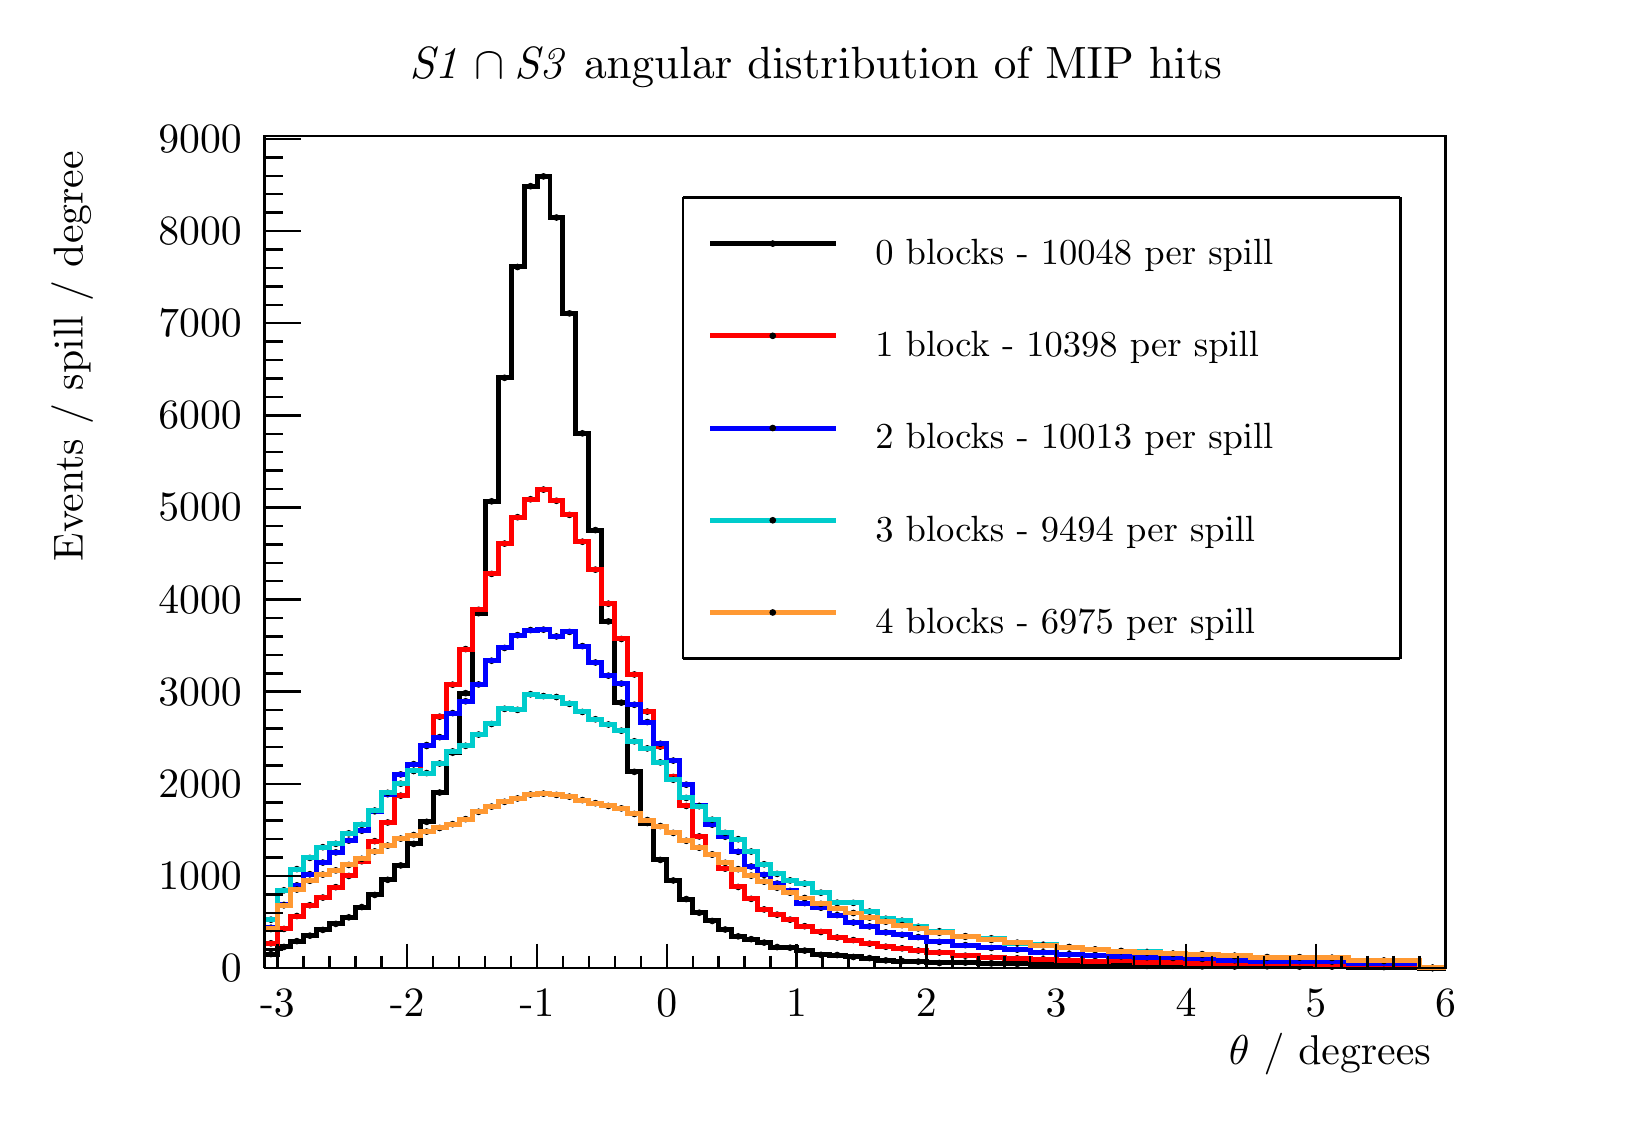
\begin{tikzpicture}
\pgfdeclareplotmark{cross} {
\pgfpathmoveto{\pgfpoint{-0.3\pgfplotmarksize}{\pgfplotmarksize}}
\pgfpathlineto{\pgfpoint{+0.3\pgfplotmarksize}{\pgfplotmarksize}}
\pgfpathlineto{\pgfpoint{+0.3\pgfplotmarksize}{0.3\pgfplotmarksize}}
\pgfpathlineto{\pgfpoint{+1\pgfplotmarksize}{0.3\pgfplotmarksize}}
\pgfpathlineto{\pgfpoint{+1\pgfplotmarksize}{-0.3\pgfplotmarksize}}
\pgfpathlineto{\pgfpoint{+0.3\pgfplotmarksize}{-0.3\pgfplotmarksize}}
\pgfpathlineto{\pgfpoint{+0.3\pgfplotmarksize}{-1.\pgfplotmarksize}}
\pgfpathlineto{\pgfpoint{-0.3\pgfplotmarksize}{-1.\pgfplotmarksize}}
\pgfpathlineto{\pgfpoint{-0.3\pgfplotmarksize}{-0.3\pgfplotmarksize}}
\pgfpathlineto{\pgfpoint{-1.\pgfplotmarksize}{-0.3\pgfplotmarksize}}
\pgfpathlineto{\pgfpoint{-1.\pgfplotmarksize}{0.3\pgfplotmarksize}}
\pgfpathlineto{\pgfpoint{-0.3\pgfplotmarksize}{0.3\pgfplotmarksize}}
\pgfpathclose
\pgfusepathqstroke
}
\pgfdeclareplotmark{cross*} {
\pgfpathmoveto{\pgfpoint{-0.3\pgfplotmarksize}{\pgfplotmarksize}}
\pgfpathlineto{\pgfpoint{+0.3\pgfplotmarksize}{\pgfplotmarksize}}
\pgfpathlineto{\pgfpoint{+0.3\pgfplotmarksize}{0.3\pgfplotmarksize}}
\pgfpathlineto{\pgfpoint{+1\pgfplotmarksize}{0.3\pgfplotmarksize}}
\pgfpathlineto{\pgfpoint{+1\pgfplotmarksize}{-0.3\pgfplotmarksize}}
\pgfpathlineto{\pgfpoint{+0.3\pgfplotmarksize}{-0.3\pgfplotmarksize}}
\pgfpathlineto{\pgfpoint{+0.3\pgfplotmarksize}{-1.\pgfplotmarksize}}
\pgfpathlineto{\pgfpoint{-0.3\pgfplotmarksize}{-1.\pgfplotmarksize}}
\pgfpathlineto{\pgfpoint{-0.3\pgfplotmarksize}{-0.3\pgfplotmarksize}}
\pgfpathlineto{\pgfpoint{-1.\pgfplotmarksize}{-0.3\pgfplotmarksize}}
\pgfpathlineto{\pgfpoint{-1.\pgfplotmarksize}{0.3\pgfplotmarksize}}
\pgfpathlineto{\pgfpoint{-0.3\pgfplotmarksize}{0.3\pgfplotmarksize}}
\pgfpathclose
\pgfusepathqfillstroke
}
\pgfdeclareplotmark{newstar} {
\pgfpathmoveto{\pgfqpoint{0pt}{\pgfplotmarksize}}
\pgfpathlineto{\pgfqpointpolar{44}{0.5\pgfplotmarksize}}
\pgfpathlineto{\pgfqpointpolar{18}{\pgfplotmarksize}}
\pgfpathlineto{\pgfqpointpolar{-20}{0.5\pgfplotmarksize}}
\pgfpathlineto{\pgfqpointpolar{-54}{\pgfplotmarksize}}
\pgfpathlineto{\pgfqpointpolar{-90}{0.5\pgfplotmarksize}}
\pgfpathlineto{\pgfqpointpolar{234}{\pgfplotmarksize}}
\pgfpathlineto{\pgfqpointpolar{198}{0.5\pgfplotmarksize}}
\pgfpathlineto{\pgfqpointpolar{162}{\pgfplotmarksize}}
\pgfpathlineto{\pgfqpointpolar{134}{0.5\pgfplotmarksize}}
\pgfpathclose
\pgfusepathqstroke
}
\pgfdeclareplotmark{newstar*} {
\pgfpathmoveto{\pgfqpoint{0pt}{\pgfplotmarksize}}
\pgfpathlineto{\pgfqpointpolar{44}{0.5\pgfplotmarksize}}
\pgfpathlineto{\pgfqpointpolar{18}{\pgfplotmarksize}}
\pgfpathlineto{\pgfqpointpolar{-20}{0.5\pgfplotmarksize}}
\pgfpathlineto{\pgfqpointpolar{-54}{\pgfplotmarksize}}
\pgfpathlineto{\pgfqpointpolar{-90}{0.5\pgfplotmarksize}}
\pgfpathlineto{\pgfqpointpolar{234}{\pgfplotmarksize}}
\pgfpathlineto{\pgfqpointpolar{198}{0.5\pgfplotmarksize}}
\pgfpathlineto{\pgfqpointpolar{162}{\pgfplotmarksize}}
\pgfpathlineto{\pgfqpointpolar{134}{0.5\pgfplotmarksize}}
\pgfpathclose
\pgfusepathqfillstroke
}
\definecolor{c}{rgb}{1,1,1};
\draw [color=c, fill=c] (0,0) rectangle (20,13.7199);
\draw [color=c, fill=c] (3,1.78359) rectangle (18,12.3479);
\definecolor{c}{rgb}{0,0,0};
\draw [c,line width=0.9] (3,1.78359) -- (3,12.3479) -- (18,12.3479) -- (18,1.78359) -- (3,1.78359);
\definecolor{c}{rgb}{1,1,1};
\draw [color=c, fill=c] (3,1.78359) rectangle (18,12.3479);
\definecolor{c}{rgb}{0,0,0};
\draw [c,line width=0.9] (3,1.78359) -- (3,12.3479) -- (18,12.3479) -- (18,1.78359) -- (3,1.78359);
\definecolor{c}{rgb}{0,0,0.6};
\draw [c,line width=0.9] (3,1.78359) -- (3.16484,1.78359) -- (3.16484,1.78359) -- (3.32967,1.78359) -- (3.32967,1.78359) -- (3.49451,1.78359) -- (3.49451,1.78359) -- (3.65934,1.78359) -- (3.65934,1.78359) -- (3.82418,1.78359) -- (3.82418,1.78359) --
 (3.98901,1.78359) -- (3.98901,1.78359) -- (4.15385,1.78359) -- (4.15385,1.78359) -- (4.31868,1.78359) -- (4.31868,1.78359) -- (4.48352,1.78359) -- (4.48352,1.78359) -- (4.64835,1.78359) -- (4.64835,1.78359) -- (4.81319,1.78359) -- (4.81319,1.78359)
 -- (4.97802,1.78359) -- (4.97802,1.78359) -- (5.14286,1.78359) -- (5.14286,1.78359) -- (5.30769,1.78359) -- (5.30769,1.78359) -- (5.47253,1.78359) -- (5.47253,1.78359) -- (5.63736,1.78359) -- (5.63736,1.78359) -- (5.8022,1.78359) -- (5.8022,1.78359)
 -- (5.96703,1.78359) -- (5.96703,1.78359) -- (6.13187,1.78359) -- (6.13187,1.78359) -- (6.2967,1.78359) -- (6.2967,1.78359) -- (6.46154,1.78359) -- (6.46154,1.78359) -- (6.62637,1.78359) -- (6.62637,1.78359) -- (6.79121,1.78359) -- (6.79121,1.78359)
 -- (6.95604,1.78359) -- (6.95604,1.78359) -- (7.12088,1.78359) -- (7.12088,1.78359) -- (7.28571,1.78359) -- (7.28571,1.78359) -- (7.45055,1.78359) -- (7.45055,1.78359) -- (7.61538,1.78359) -- (7.61538,1.78359) -- (7.78022,1.78359) --
 (7.78022,1.78359) -- (7.94506,1.78359) -- (7.94506,1.78359) -- (8.10989,1.78359) -- (8.10989,1.78359) -- (8.27472,1.78359) -- (8.27472,1.78359) -- (8.43956,1.78359) -- (8.43956,1.78359) -- (8.6044,1.78359) -- (8.6044,1.78359) -- (8.76923,1.78359) --
 (8.76923,1.78359) -- (8.93407,1.78359) -- (8.93407,1.78359) -- (9.0989,1.78359) -- (9.0989,1.78359) -- (9.26374,1.78359) -- (9.26374,1.78359) -- (9.42857,1.78359) -- (9.42857,1.78359) -- (9.59341,1.78359) -- (9.59341,1.78359) -- (9.75824,1.78359) --
 (9.75824,1.78359) -- (9.96429,1.78359) -- (9.96429,1.78359) -- (10.1703,1.78359) -- (10.1703,1.78359) -- (10.3764,1.78359) -- (10.3764,1.78359) -- (10.5824,1.78359) -- (10.5824,1.78359) -- (10.7885,1.78359) -- (10.7885,1.78359) -- (10.9945,1.78359)
 -- (10.9945,1.78359) -- (11.2005,1.78359) -- (11.2005,1.78359) -- (11.4066,1.78359) -- (11.4066,1.78359) -- (11.7363,1.78359) -- (11.7363,1.78359) -- (12.0659,1.78359) -- (12.0659,1.78359) -- (12.3956,1.78359) -- (12.3956,1.78359) --
 (12.7253,1.78359) -- (12.7253,1.78359) -- (13.0549,1.78359) -- (13.0549,1.78359) -- (13.3846,1.78359) -- (13.3846,1.78359) -- (13.7143,1.78359) -- (13.7143,1.78359) -- (14.044,1.78359) -- (14.044,1.78359) -- (14.3736,1.78359) -- (14.3736,1.78359) --
 (14.7033,1.78359) -- (14.7033,1.78359) -- (15.1154,1.78359) -- (15.1154,1.78359) -- (15.5275,1.78359) -- (15.5275,1.78359) -- (15.9396,1.78359) -- (15.9396,1.78359) -- (16.3516,1.78359) -- (16.3516,1.78359) -- (16.7637,1.78359) -- (16.7637,1.78359)
 -- (17.6703,1.78359) -- (17.6703,1.78359) -- (18,1.78359);
\definecolor{c}{rgb}{0,0,0};
\draw [c,line width=0.9] (3,1.78359) -- (18,1.78359);
\draw [c,line width=0.9] (3.16484,2.09229) -- (3.16484,1.78359);
\draw [c,line width=0.9] (3.49451,1.93794) -- (3.49451,1.78359);
\draw [c,line width=0.9] (3.82418,1.93794) -- (3.82418,1.78359);
\draw [c,line width=0.9] (4.15385,1.93794) -- (4.15385,1.78359);
\draw [c,line width=0.9] (4.48352,1.93794) -- (4.48352,1.78359);
\draw [c,line width=0.9] (4.81319,2.09229) -- (4.81319,1.78359);
\draw [c,line width=0.9] (5.14286,1.93794) -- (5.14286,1.78359);
\draw [c,line width=0.9] (5.47253,1.93794) -- (5.47253,1.78359);
\draw [c,line width=0.9] (5.8022,1.93794) -- (5.8022,1.78359);
\draw [c,line width=0.9] (6.13187,1.93794) -- (6.13187,1.78359);
\draw [c,line width=0.9] (6.46154,2.09229) -- (6.46154,1.78359);
\draw [c,line width=0.9] (6.79121,1.93794) -- (6.79121,1.78359);
\draw [c,line width=0.9] (7.12088,1.93794) -- (7.12088,1.78359);
\draw [c,line width=0.9] (7.45055,1.93794) -- (7.45055,1.78359);
\draw [c,line width=0.9] (7.78022,1.93794) -- (7.78022,1.78359);
\draw [c,line width=0.9] (8.10989,2.09229) -- (8.10989,1.78359);
\draw [c,line width=0.9] (8.43956,1.93794) -- (8.43956,1.78359);
\draw [c,line width=0.9] (8.76923,1.93794) -- (8.76923,1.78359);
\draw [c,line width=0.9] (9.0989,1.93794) -- (9.0989,1.78359);
\draw [c,line width=0.9] (9.42857,1.93794) -- (9.42857,1.78359);
\draw [c,line width=0.9] (9.75824,2.09229) -- (9.75824,1.78359);
\draw [c,line width=0.9] (10.0879,1.93794) -- (10.0879,1.78359);
\draw [c,line width=0.9] (10.4176,1.93794) -- (10.4176,1.78359);
\draw [c,line width=0.9] (10.7473,1.93794) -- (10.7473,1.78359);
\draw [c,line width=0.9] (11.0769,1.93794) -- (11.0769,1.78359);
\draw [c,line width=0.9] (11.4066,2.09229) -- (11.4066,1.78359);
\draw [c,line width=0.9] (11.7363,1.93794) -- (11.7363,1.78359);
\draw [c,line width=0.9] (12.0659,1.93794) -- (12.0659,1.78359);
\draw [c,line width=0.9] (12.3956,1.93794) -- (12.3956,1.78359);
\draw [c,line width=0.9] (12.7253,1.93794) -- (12.7253,1.78359);
\draw [c,line width=0.9] (13.0549,2.09229) -- (13.0549,1.78359);
\draw [c,line width=0.9] (13.3846,1.93794) -- (13.3846,1.78359);
\draw [c,line width=0.9] (13.7143,1.93794) -- (13.7143,1.78359);
\draw [c,line width=0.9] (14.044,1.93794) -- (14.044,1.78359);
\draw [c,line width=0.9] (14.3736,1.93794) -- (14.3736,1.78359);
\draw [c,line width=0.9] (14.7033,2.09229) -- (14.7033,1.78359);
\draw [c,line width=0.9] (15.033,1.93794) -- (15.033,1.78359);
\draw [c,line width=0.9] (15.3626,1.93794) -- (15.3626,1.78359);
\draw [c,line width=0.9] (15.6923,1.93794) -- (15.6923,1.78359);
\draw [c,line width=0.9] (16.022,1.93794) -- (16.022,1.78359);
\draw [c,line width=0.9] (16.3516,2.09229) -- (16.3516,1.78359);
\draw [c,line width=0.9] (16.6813,1.93794) -- (16.6813,1.78359);
\draw [c,line width=0.9] (17.011,1.93794) -- (17.011,1.78359);
\draw [c,line width=0.9] (17.3407,1.93794) -- (17.3407,1.78359);
\draw [c,line width=0.9] (17.6703,1.93794) -- (17.6703,1.78359);
\draw [c,line width=0.9] (18,2.09229) -- (18,1.78359);
\draw [c,line width=0.9] (3.16484,2.09229) -- (3.16484,1.78359);
\draw [anchor=base] (3.16484,1.1662) node[scale=1.50787, color=c, rotate=0]{-3};
\draw [anchor=base] (4.81319,1.1662) node[scale=1.50787, color=c, rotate=0]{-2};
\draw [anchor=base] (6.46154,1.1662) node[scale=1.50787, color=c, rotate=0]{-1};
\draw [anchor=base] (8.10989,1.1662) node[scale=1.50787, color=c, rotate=0]{0};
\draw [anchor=base] (9.75824,1.1662) node[scale=1.50787, color=c, rotate=0]{1};
\draw [anchor=base] (11.4066,1.1662) node[scale=1.50787, color=c, rotate=0]{2};
\draw [anchor=base] (13.0549,1.1662) node[scale=1.50787, color=c, rotate=0]{3};
\draw [anchor=base] (14.7033,1.1662) node[scale=1.50787, color=c, rotate=0]{4};
\draw [anchor=base] (16.3516,1.1662) node[scale=1.50787, color=c, rotate=0]{5};
\draw [anchor=base] (18,1.1662) node[scale=1.50787, color=c, rotate=0]{6};
\draw [anchor= east] (18,0.685997) node[scale=1.50787, color=c, rotate=0]{$\theta$ / degrees};
\draw [c,line width=0.9] (3,1.78359) -- (3,12.3479);
\draw [c,line width=0.9] (3.462,1.78359) -- (3,1.78359);
\draw [c,line width=0.9] (3.231,2.01758) -- (3,2.01758);
\draw [c,line width=0.9] (3.231,2.25157) -- (3,2.25157);
\draw [c,line width=0.9] (3.231,2.48557) -- (3,2.48557);
\draw [c,line width=0.9] (3.231,2.71956) -- (3,2.71956);
\draw [c,line width=0.9] (3.462,2.95355) -- (3,2.95355);
\draw [c,line width=0.9] (3.231,3.18754) -- (3,3.18754);
\draw [c,line width=0.9] (3.231,3.42153) -- (3,3.42153);
\draw [c,line width=0.9] (3.231,3.65552) -- (3,3.65552);
\draw [c,line width=0.9] (3.231,3.88951) -- (3,3.88951);
\draw [c,line width=0.9] (3.462,4.1235) -- (3,4.1235);
\draw [c,line width=0.9] (3.231,4.35749) -- (3,4.35749);
\draw [c,line width=0.9] (3.231,4.59148) -- (3,4.59148);
\draw [c,line width=0.9] (3.231,4.82548) -- (3,4.82548);
\draw [c,line width=0.9] (3.231,5.05947) -- (3,5.05947);
\draw [c,line width=0.9] (3.462,5.29346) -- (3,5.29346);
\draw [c,line width=0.9] (3.231,5.52745) -- (3,5.52745);
\draw [c,line width=0.9] (3.231,5.76144) -- (3,5.76144);
\draw [c,line width=0.9] (3.231,5.99543) -- (3,5.99543);
\draw [c,line width=0.9] (3.231,6.22942) -- (3,6.22942);
\draw [c,line width=0.9] (3.462,6.46341) -- (3,6.46341);
\draw [c,line width=0.9] (3.231,6.6974) -- (3,6.6974);
\draw [c,line width=0.9] (3.231,6.93139) -- (3,6.93139);
\draw [c,line width=0.9] (3.231,7.16539) -- (3,7.16539);
\draw [c,line width=0.9] (3.231,7.39938) -- (3,7.39938);
\draw [c,line width=0.9] (3.462,7.63337) -- (3,7.63337);
\draw [c,line width=0.9] (3.231,7.86736) -- (3,7.86736);
\draw [c,line width=0.9] (3.231,8.10135) -- (3,8.10135);
\draw [c,line width=0.9] (3.231,8.33534) -- (3,8.33534);
\draw [c,line width=0.9] (3.231,8.56933) -- (3,8.56933);
\draw [c,line width=0.9] (3.462,8.80332) -- (3,8.80332);
\draw [c,line width=0.9] (3.231,9.03731) -- (3,9.03731);
\draw [c,line width=0.9] (3.231,9.27131) -- (3,9.27131);
\draw [c,line width=0.9] (3.231,9.5053) -- (3,9.5053);
\draw [c,line width=0.9] (3.231,9.73929) -- (3,9.73929);
\draw [c,line width=0.9] (3.462,9.97328) -- (3,9.97328);
\draw [c,line width=0.9] (3.231,10.2073) -- (3,10.2073);
\draw [c,line width=0.9] (3.231,10.4413) -- (3,10.4413);
\draw [c,line width=0.9] (3.231,10.6753) -- (3,10.6753);
\draw [c,line width=0.9] (3.231,10.9092) -- (3,10.9092);
\draw [c,line width=0.9] (3.462,11.1432) -- (3,11.1432);
\draw [c,line width=0.9] (3.231,11.3772) -- (3,11.3772);
\draw [c,line width=0.9] (3.231,11.6112) -- (3,11.6112);
\draw [c,line width=0.9] (3.231,11.8452) -- (3,11.8452);
\draw [c,line width=0.9] (3.231,12.0792) -- (3,12.0792);
\draw [c,line width=0.9] (3.462,12.3132) -- (3,12.3132);
\draw [c,line width=0.9] (3.462,12.3132) -- (3,12.3132);
\draw [anchor= east] (2.9,1.78359) node[scale=1.50787, color=c, rotate=0]{0};
\draw [anchor= east] (2.9,2.95355) node[scale=1.50787, color=c, rotate=0]{1000};
\draw [anchor= east] (2.9,4.1235) node[scale=1.50787, color=c, rotate=0]{2000};
\draw [anchor= east] (2.9,5.29346) node[scale=1.50787, color=c, rotate=0]{3000};
\draw [anchor= east] (2.9,6.46341) node[scale=1.50787, color=c, rotate=0]{4000};
\draw [anchor= east] (2.9,7.63337) node[scale=1.50787, color=c, rotate=0]{5000};
\draw [anchor= east] (2.9,8.80332) node[scale=1.50787, color=c, rotate=0]{6000};
\draw [anchor= east] (2.9,9.97328) node[scale=1.50787, color=c, rotate=0]{7000};
\draw [anchor= east] (2.9,11.1432) node[scale=1.50787, color=c, rotate=0]{8000};
\draw [anchor= east] (2.9,12.3132) node[scale=1.50787, color=c, rotate=0]{9000};
\draw [anchor= east] (0.557284,12.3479) node[scale=1.50787, color=c, rotate=90]{ Events / spill / degree};
\draw [c,line width=1.8] (3.08242,1.96042) -- (3.08242,1.96133);
\draw [c,line width=1.8] (3.08242,1.96133) -- (3.08242,1.96225);
\foreach \P in {(3.08242,1.96133)}{\draw[mark options={color=c,fill=c},mark size=2.402402pt,mark=*,mark size=1pt] plot coordinates {\P};}
\draw [c,line width=1.8] (3.24725,2.05096) -- (3.24725,2.05209);
\draw [c,line width=1.8] (3.24725,2.05209) -- (3.24725,2.05321);
\foreach \P in {(3.24725,2.05209)}{\draw[mark options={color=c,fill=c},mark size=2.402402pt,mark=*,mark size=1pt] plot coordinates {\P};}
\draw [c,line width=1.8] (3.41209,2.1247) -- (3.41209,2.12597);
\draw [c,line width=1.8] (3.41209,2.12597) -- (3.41209,2.12724);
\foreach \P in {(3.41209,2.12597)}{\draw[mark options={color=c,fill=c},mark size=2.402402pt,mark=*,mark size=1pt] plot coordinates {\P};}
\draw [c,line width=1.8] (3.57692,2.19382) -- (3.57692,2.19522);
\draw [c,line width=1.8] (3.57692,2.19522) -- (3.57692,2.19662);
\foreach \P in {(3.57692,2.19522)}{\draw[mark options={color=c,fill=c},mark size=2.402402pt,mark=*,mark size=1pt] plot coordinates {\P};}
\draw [c,line width=1.8] (3.74176,2.26714) -- (3.74176,2.26865);
\draw [c,line width=1.8] (3.74176,2.26865) -- (3.74176,2.27017);
\foreach \P in {(3.74176,2.26865)}{\draw[mark options={color=c,fill=c},mark size=2.402402pt,mark=*,mark size=1pt] plot coordinates {\P};}
\draw [c,line width=1.8] (3.90659,2.34336) -- (3.90659,2.34499);
\draw [c,line width=1.8] (3.90659,2.34499) -- (3.90659,2.34662);
\foreach \P in {(3.90659,2.34499)}{\draw[mark options={color=c,fill=c},mark size=2.402402pt,mark=*,mark size=1pt] plot coordinates {\P};}
\draw [c,line width=1.8] (4.07143,2.42657) -- (4.07143,2.42831);
\draw [c,line width=1.8] (4.07143,2.42831) -- (4.07143,2.43004);
\foreach \P in {(4.07143,2.42831)}{\draw[mark options={color=c,fill=c},mark size=2.402402pt,mark=*,mark size=1pt] plot coordinates {\P};}
\draw [c,line width=1.8] (4.23626,2.55668) -- (4.23626,2.55859);
\draw [c,line width=1.8] (4.23626,2.55859) -- (4.23626,2.5605);
\foreach \P in {(4.23626,2.55859)}{\draw[mark options={color=c,fill=c},mark size=2.402402pt,mark=*,mark size=1pt] plot coordinates {\P};}
\draw [c,line width=1.8] (4.4011,2.71038) -- (4.4011,2.71247);
\draw [c,line width=1.8] (4.4011,2.71247) -- (4.4011,2.71456);
\foreach \P in {(4.4011,2.71247)}{\draw[mark options={color=c,fill=c},mark size=2.402402pt,mark=*,mark size=1pt] plot coordinates {\P};}
\draw [c,line width=1.8] (4.56593,2.90221) -- (4.56593,2.90451);
\draw [c,line width=1.8] (4.56593,2.90451) -- (4.56593,2.90682);
\foreach \P in {(4.56593,2.90451)}{\draw[mark options={color=c,fill=c},mark size=2.402402pt,mark=*,mark size=1pt] plot coordinates {\P};}
\draw [c,line width=1.8] (4.73077,3.08496) -- (4.73077,3.08744);
\draw [c,line width=1.8] (4.73077,3.08744) -- (4.73077,3.08992);
\foreach \P in {(4.73077,3.08744)}{\draw[mark options={color=c,fill=c},mark size=2.402402pt,mark=*,mark size=1pt] plot coordinates {\P};}
\draw [c,line width=1.8] (4.8956,3.35822) -- (4.8956,3.36094);
\draw [c,line width=1.8] (4.8956,3.36094) -- (4.8956,3.36367);
\foreach \P in {(4.8956,3.36094)}{\draw[mark options={color=c,fill=c},mark size=2.402402pt,mark=*,mark size=1pt] plot coordinates {\P};}
\draw [c,line width=1.8] (5.06044,3.63804) -- (5.06044,3.641);
\draw [c,line width=1.8] (5.06044,3.641) -- (5.06044,3.64396);
\foreach \P in {(5.06044,3.641)}{\draw[mark options={color=c,fill=c},mark size=2.402402pt,mark=*,mark size=1pt] plot coordinates {\P};}
\draw [c,line width=1.8] (5.22528,4.00993) -- (5.22528,4.01317);
\draw [c,line width=1.8] (5.22528,4.01317) -- (5.22528,4.01641);
\foreach \P in {(5.22528,4.01317)}{\draw[mark options={color=c,fill=c},mark size=2.402402pt,mark=*,mark size=1pt] plot coordinates {\P};}
\draw [c,line width=1.8] (5.39011,4.5153) -- (5.39011,4.5189);
\draw [c,line width=1.8] (5.39011,4.5189) -- (5.39011,4.52249);
\foreach \P in {(5.39011,4.5189)}{\draw[mark options={color=c,fill=c},mark size=2.402402pt,mark=*,mark size=1pt] plot coordinates {\P};}
\draw [c,line width=1.8] (5.55494,5.27113) -- (5.55494,5.27519);
\draw [c,line width=1.8] (5.55494,5.27519) -- (5.55494,5.27926);
\foreach \P in {(5.55494,5.27519)}{\draw[mark options={color=c,fill=c},mark size=2.402402pt,mark=*,mark size=1pt] plot coordinates {\P};}
\draw [c,line width=1.8] (5.71978,6.28683) -- (5.71978,6.29145);
\draw [c,line width=1.8] (5.71978,6.29145) -- (5.71978,6.29606);
\foreach \P in {(5.71978,6.29145)}{\draw[mark options={color=c,fill=c},mark size=2.402402pt,mark=*,mark size=1pt] plot coordinates {\P};}
\draw [c,line width=1.8] (5.88462,7.70618) -- (5.88462,7.71147);
\draw [c,line width=1.8] (5.88462,7.71147) -- (5.88462,7.71676);
\foreach \P in {(5.88462,7.71147)}{\draw[mark options={color=c,fill=c},mark size=2.402402pt,mark=*,mark size=1pt] plot coordinates {\P};}
\draw [c,line width=1.8] (6.04945,9.27429) -- (6.04945,9.28024);
\draw [c,line width=1.8] (6.04945,9.28024) -- (6.04945,9.28619);
\foreach \P in {(6.04945,9.28024)}{\draw[mark options={color=c,fill=c},mark size=2.402402pt,mark=*,mark size=1pt] plot coordinates {\P};}
\draw [c,line width=1.8] (6.21429,10.681) -- (6.21429,10.6875);
\draw [c,line width=1.8] (6.21429,10.6875) -- (6.21429,10.694);
\foreach \P in {(6.21429,10.6875)}{\draw[mark options={color=c,fill=c},mark size=2.402402pt,mark=*,mark size=1pt] plot coordinates {\P};}
\draw [c,line width=1.8] (6.37912,11.7069) -- (6.37912,11.7137);
\draw [c,line width=1.8] (6.37912,11.7137) -- (6.37912,11.7206);
\foreach \P in {(6.37912,11.7137)}{\draw[mark options={color=c,fill=c},mark size=2.402402pt,mark=*,mark size=1pt] plot coordinates {\P};}
\draw [c,line width=1.8] (6.54396,11.8311) -- (6.54396,11.838);
\draw [c,line width=1.8] (6.54396,11.838) -- (6.54396,11.8449);
\foreach \P in {(6.54396,11.838)}{\draw[mark options={color=c,fill=c},mark size=2.402402pt,mark=*,mark size=1pt] plot coordinates {\P};}
\draw [c,line width=1.8] (6.70879,11.3088) -- (6.70879,11.3155);
\draw [c,line width=1.8] (6.70879,11.3155) -- (6.70879,11.3222);
\foreach \P in {(6.70879,11.3155)}{\draw[mark options={color=c,fill=c},mark size=2.402402pt,mark=*,mark size=1pt] plot coordinates {\P};}
\draw [c,line width=1.8] (6.87363,10.0921) -- (6.87363,10.0984);
\draw [c,line width=1.8] (6.87363,10.0984) -- (6.87363,10.1047);
\foreach \P in {(6.87363,10.0984)}{\draw[mark options={color=c,fill=c},mark size=2.402402pt,mark=*,mark size=1pt] plot coordinates {\P};}
\draw [c,line width=1.8] (7.03846,8.56933) -- (7.03846,8.575);
\draw [c,line width=1.8] (7.03846,8.575) -- (7.03846,8.58066);
\foreach \P in {(7.03846,8.575)}{\draw[mark options={color=c,fill=c},mark size=2.402402pt,mark=*,mark size=1pt] plot coordinates {\P};}
\draw [c,line width=1.8] (7.2033,7.34089) -- (7.2033,7.34602);
\draw [c,line width=1.8] (7.2033,7.34602) -- (7.2033,7.35115);
\foreach \P in {(7.2033,7.34602)}{\draw[mark options={color=c,fill=c},mark size=2.402402pt,mark=*,mark size=1pt] plot coordinates {\P};}
\draw [c,line width=1.8] (7.36813,6.1819) -- (7.36813,6.18646);
\draw [c,line width=1.8] (7.36813,6.18646) -- (7.36813,6.19101);
\foreach \P in {(7.36813,6.18646)}{\draw[mark options={color=c,fill=c},mark size=2.402402pt,mark=*,mark size=1pt] plot coordinates {\P};}
\draw [c,line width=1.8] (7.53297,5.15058) -- (7.53297,5.15457);
\draw [c,line width=1.8] (7.53297,5.15457) -- (7.53297,5.15856);
\foreach \P in {(7.53297,5.15457)}{\draw[mark options={color=c,fill=c},mark size=2.402402pt,mark=*,mark size=1pt] plot coordinates {\P};}
\draw [c,line width=1.8] (7.6978,4.27259) -- (7.6978,4.27602);
\draw [c,line width=1.8] (7.6978,4.27602) -- (7.6978,4.27944);
\foreach \P in {(7.6978,4.27602)}{\draw[mark options={color=c,fill=c},mark size=2.402402pt,mark=*,mark size=1pt] plot coordinates {\P};}
\draw [c,line width=1.8] (7.86264,3.62309) -- (7.86264,3.62604);
\draw [c,line width=1.8] (7.86264,3.62604) -- (7.86264,3.62899);
\foreach \P in {(7.86264,3.62604)}{\draw[mark options={color=c,fill=c},mark size=2.402402pt,mark=*,mark size=1pt] plot coordinates {\P};}
\draw [c,line width=1.8] (8.02747,3.15496) -- (8.02747,3.15751);
\draw [c,line width=1.8] (8.02747,3.15751) -- (8.02747,3.16006);
\foreach \P in {(8.02747,3.15751)}{\draw[mark options={color=c,fill=c},mark size=2.402402pt,mark=*,mark size=1pt] plot coordinates {\P};}
\draw [c,line width=1.8] (8.19231,2.89398) -- (8.19231,2.89627);
\draw [c,line width=1.8] (8.19231,2.89627) -- (8.19231,2.89856);
\foreach \P in {(8.19231,2.89627)}{\draw[mark options={color=c,fill=c},mark size=2.402402pt,mark=*,mark size=1pt] plot coordinates {\P};}
\draw [c,line width=1.8] (8.35714,2.65818) -- (8.35714,2.66022);
\draw [c,line width=1.8] (8.35714,2.66022) -- (8.35714,2.66225);
\foreach \P in {(8.35714,2.66022)}{\draw[mark options={color=c,fill=c},mark size=2.402402pt,mark=*,mark size=1pt] plot coordinates {\P};}
\draw [c,line width=1.8] (8.52198,2.48491) -- (8.52198,2.48674);
\draw [c,line width=1.8] (8.52198,2.48674) -- (8.52198,2.48857);
\foreach \P in {(8.52198,2.48674)}{\draw[mark options={color=c,fill=c},mark size=2.402402pt,mark=*,mark size=1pt] plot coordinates {\P};}
\draw [c,line width=1.8] (8.68681,2.38063) -- (8.68681,2.38232);
\draw [c,line width=1.8] (8.68681,2.38232) -- (8.68681,2.384);
\foreach \P in {(8.68681,2.38232)}{\draw[mark options={color=c,fill=c},mark size=2.402402pt,mark=*,mark size=1pt] plot coordinates {\P};}
\draw [c,line width=1.8] (8.85165,2.272) -- (8.85165,2.27352);
\draw [c,line width=1.8] (8.85165,2.27352) -- (8.85165,2.27504);
\foreach \P in {(8.85165,2.27352)}{\draw[mark options={color=c,fill=c},mark size=2.402402pt,mark=*,mark size=1pt] plot coordinates {\P};}
\draw [c,line width=1.8] (9.01648,2.18553) -- (9.01648,2.18691);
\draw [c,line width=1.8] (9.01648,2.18691) -- (9.01648,2.1883);
\foreach \P in {(9.01648,2.18691)}{\draw[mark options={color=c,fill=c},mark size=2.402402pt,mark=*,mark size=1pt] plot coordinates {\P};}
\draw [c,line width=1.8] (9.18132,2.14992) -- (9.18132,2.15123);
\draw [c,line width=1.8] (9.18132,2.15123) -- (9.18132,2.15255);
\foreach \P in {(9.18132,2.15123)}{\draw[mark options={color=c,fill=c},mark size=2.402402pt,mark=*,mark size=1pt] plot coordinates {\P};}
\draw [c,line width=1.8] (9.34615,2.10613) -- (9.34615,2.10737);
\draw [c,line width=1.8] (9.34615,2.10737) -- (9.34615,2.10861);
\foreach \P in {(9.34615,2.10737)}{\draw[mark options={color=c,fill=c},mark size=2.402402pt,mark=*,mark size=1pt] plot coordinates {\P};}
\draw [c,line width=1.8] (9.51099,2.04971) -- (9.51099,2.05084);
\draw [c,line width=1.8] (9.51099,2.05084) -- (9.51099,2.05196);
\foreach \P in {(9.51099,2.05084)}{\draw[mark options={color=c,fill=c},mark size=2.402402pt,mark=*,mark size=1pt] plot coordinates {\P};}
\draw [c,line width=1.8] (9.67582,2.04139) -- (9.67582,2.0425);
\draw [c,line width=1.8] (9.67582,2.0425) -- (9.67582,2.04362);
\foreach \P in {(9.67582,2.0425)}{\draw[mark options={color=c,fill=c},mark size=2.402402pt,mark=*,mark size=1pt] plot coordinates {\P};}
\draw [c,line width=1.8] (9.86126,2.00446) -- (9.86126,2.0056);
\draw [c,line width=1.8] (9.86126,2.0056) -- (9.86126,2.00675);
\foreach \P in {(9.86126,2.0056)}{\draw[mark options={color=c,fill=c},mark size=2.402402pt,mark=*,mark size=1pt] plot coordinates {\P};}
\draw [c,line width=1.8] (10.0673,1.95095) -- (10.0673,1.95195);
\draw [c,line width=1.8] (10.0673,1.95195) -- (10.0673,1.95295);
\foreach \P in {(10.0673,1.95195)}{\draw[mark options={color=c,fill=c},mark size=2.402402pt,mark=*,mark size=1pt] plot coordinates {\P};}
\draw [c,line width=1.8] (10.2734,1.94837) -- (10.2734,1.94936);
\draw [c,line width=1.8] (10.2734,1.94936) -- (10.2734,1.95035);
\foreach \P in {(10.2734,1.94936)}{\draw[mark options={color=c,fill=c},mark size=2.402402pt,mark=*,mark size=1pt] plot coordinates {\P};}
\draw [c,line width=1.8] (10.4794,1.92407) -- (10.4794,1.92498);
\draw [c,line width=1.8] (10.4794,1.92498) -- (10.4794,1.92589);
\foreach \P in {(10.4794,1.92498)}{\draw[mark options={color=c,fill=c},mark size=2.402402pt,mark=*,mark size=1pt] plot coordinates {\P};}
\draw [c,line width=1.8] (10.6854,1.90959) -- (10.6854,1.91046);
\draw [c,line width=1.8] (10.6854,1.91046) -- (10.6854,1.91133);
\foreach \P in {(10.6854,1.91046)}{\draw[mark options={color=c,fill=c},mark size=2.402402pt,mark=*,mark size=1pt] plot coordinates {\P};}
\draw [c,line width=1.8] (10.8915,1.88035) -- (10.8915,1.88111);
\draw [c,line width=1.8] (10.8915,1.88111) -- (10.8915,1.88187);
\foreach \P in {(10.8915,1.88111)}{\draw[mark options={color=c,fill=c},mark size=2.402402pt,mark=*,mark size=1pt] plot coordinates {\P};}
\draw [c,line width=1.8] (11.0975,1.87278) -- (11.0975,1.87351);
\draw [c,line width=1.8] (11.0975,1.87351) -- (11.0975,1.87424);
\foreach \P in {(11.0975,1.87351)}{\draw[mark options={color=c,fill=c},mark size=2.402402pt,mark=*,mark size=1pt] plot coordinates {\P};}
\draw [c,line width=1.8] (11.3036,1.86516) -- (11.3036,1.86587);
\draw [c,line width=1.8] (11.3036,1.86587) -- (11.3036,1.86657);
\foreach \P in {(11.3036,1.86587)}{\draw[mark options={color=c,fill=c},mark size=2.402402pt,mark=*,mark size=1pt] plot coordinates {\P};}
\draw [c,line width=1.8] (11.5714,1.8481) -- (11.5714,1.84889);
\draw [c,line width=1.8] (11.5714,1.84889) -- (11.5714,1.84967);
\foreach \P in {(11.5714,1.84889)}{\draw[mark options={color=c,fill=c},mark size=2.402402pt,mark=*,mark size=1pt] plot coordinates {\P};}
\draw [c,line width=1.8] (11.9011,1.85223) -- (11.9011,1.85304);
\draw [c,line width=1.8] (11.9011,1.85304) -- (11.9011,1.85385);
\foreach \P in {(11.9011,1.85304)}{\draw[mark options={color=c,fill=c},mark size=2.402402pt,mark=*,mark size=1pt] plot coordinates {\P};}
\draw [c,line width=1.8] (12.2308,1.84206) -- (12.2308,1.84281);
\draw [c,line width=1.8] (12.2308,1.84281) -- (12.2308,1.84356);
\foreach \P in {(12.2308,1.84281)}{\draw[mark options={color=c,fill=c},mark size=2.402402pt,mark=*,mark size=1pt] plot coordinates {\P};}
\draw [c,line width=1.8] (12.5604,1.83622) -- (12.5604,1.83693);
\draw [c,line width=1.8] (12.5604,1.83693) -- (12.5604,1.83764);
\foreach \P in {(12.5604,1.83693)}{\draw[mark options={color=c,fill=c},mark size=2.402402pt,mark=*,mark size=1pt] plot coordinates {\P};}
\draw [c,line width=1.8] (12.8901,1.82585) -- (12.8901,1.82649);
\draw [c,line width=1.8] (12.8901,1.82649) -- (12.8901,1.82713);
\foreach \P in {(12.8901,1.82649)}{\draw[mark options={color=c,fill=c},mark size=2.402402pt,mark=*,mark size=1pt] plot coordinates {\P};}
\draw [c,line width=1.8] (13.2198,1.82341) -- (13.2198,1.82402);
\draw [c,line width=1.8] (13.2198,1.82402) -- (13.2198,1.82464);
\foreach \P in {(13.2198,1.82402)}{\draw[mark options={color=c,fill=c},mark size=2.402402pt,mark=*,mark size=1pt] plot coordinates {\P};}
\draw [c,line width=1.8] (13.5495,1.81898) -- (13.5495,1.81956);
\draw [c,line width=1.8] (13.5495,1.81956) -- (13.5495,1.82014);
\foreach \P in {(13.5495,1.81956)}{\draw[mark options={color=c,fill=c},mark size=2.402402pt,mark=*,mark size=1pt] plot coordinates {\P};}
\draw [c,line width=1.8] (13.8791,1.81696) -- (13.8791,1.81754);
\draw [c,line width=1.8] (13.8791,1.81754) -- (13.8791,1.81812);
\foreach \P in {(13.8791,1.81754)}{\draw[mark options={color=c,fill=c},mark size=2.402402pt,mark=*,mark size=1pt] plot coordinates {\P};}
\draw [c,line width=1.8] (14.2088,1.81084) -- (14.2088,1.81136);
\draw [c,line width=1.8] (14.2088,1.81136) -- (14.2088,1.81187);
\foreach \P in {(14.2088,1.81136)}{\draw[mark options={color=c,fill=c},mark size=2.402402pt,mark=*,mark size=1pt] plot coordinates {\P};}
\draw [c,line width=1.8] (14.5385,1.81226) -- (14.5385,1.81279);
\draw [c,line width=1.8] (14.5385,1.81279) -- (14.5385,1.81331);
\foreach \P in {(14.5385,1.81279)}{\draw[mark options={color=c,fill=c},mark size=2.402402pt,mark=*,mark size=1pt] plot coordinates {\P};}
\draw [c,line width=1.8] (14.9093,1.80551) -- (14.9093,1.80603);
\draw [c,line width=1.8] (14.9093,1.80603) -- (14.9093,1.80656);
\foreach \P in {(14.9093,1.80603)}{\draw[mark options={color=c,fill=c},mark size=2.402402pt,mark=*,mark size=1pt] plot coordinates {\P};}
\draw [c,line width=1.8] (15.3214,1.80324) -- (15.3214,1.80373);
\draw [c,line width=1.8] (15.3214,1.80373) -- (15.3214,1.80421);
\foreach \P in {(15.3214,1.80373)}{\draw[mark options={color=c,fill=c},mark size=2.402402pt,mark=*,mark size=1pt] plot coordinates {\P};}
\draw [c,line width=1.8] (15.7335,1.80624) -- (15.7335,1.80676);
\draw [c,line width=1.8] (15.7335,1.80676) -- (15.7335,1.80729);
\foreach \P in {(15.7335,1.80676)}{\draw[mark options={color=c,fill=c},mark size=2.402402pt,mark=*,mark size=1pt] plot coordinates {\P};}
\draw [c,line width=1.8] (16.1456,1.80134) -- (16.1456,1.8018);
\draw [c,line width=1.8] (16.1456,1.8018) -- (16.1456,1.80227);
\foreach \P in {(16.1456,1.8018)}{\draw[mark options={color=c,fill=c},mark size=2.402402pt,mark=*,mark size=1pt] plot coordinates {\P};}
\draw [c,line width=1.8] (16.5577,1.80172) -- (16.5577,1.80219);
\draw [c,line width=1.8] (16.5577,1.80219) -- (16.5577,1.80265);
\foreach \P in {(16.5577,1.80219)}{\draw[mark options={color=c,fill=c},mark size=2.402402pt,mark=*,mark size=1pt] plot coordinates {\P};}
\draw [c,line width=1.8] (17.217,1.79545) -- (17.217,1.79602);
\draw [c,line width=1.8] (17.217,1.79602) -- (17.217,1.79658);
\foreach \P in {(17.217,1.79602)}{\draw[mark options={color=c,fill=c},mark size=2.402402pt,mark=*,mark size=1pt] plot coordinates {\P};}
\draw [c,line width=1.8] (17.8352,1.78436) -- (17.8352,1.78458);
\draw [c,line width=1.8] (17.8352,1.78458) -- (17.8352,1.7848);
\foreach \P in {(17.8352,1.78458)}{\draw[mark options={color=c,fill=c},mark size=2.402402pt,mark=*,mark size=1pt] plot coordinates {\P};}
\draw [c,line width=1.8] (3,1.96133) -- (3.16484,1.96133) -- (3.16484,2.05209) -- (3.32967,2.05209) -- (3.32967,2.12597) -- (3.49451,2.12597) -- (3.49451,2.19522) -- (3.65934,2.19522) -- (3.65934,2.26865) -- (3.82418,2.26865) -- (3.82418,2.34499) --
 (3.98901,2.34499) -- (3.98901,2.42831) -- (4.15385,2.42831) -- (4.15385,2.55859) -- (4.31868,2.55859) -- (4.31868,2.71247) -- (4.48352,2.71247) -- (4.48352,2.90451) -- (4.64835,2.90451) -- (4.64835,3.08744) -- (4.81319,3.08744) -- (4.81319,3.36094)
 -- (4.97802,3.36094) -- (4.97802,3.641) -- (5.14286,3.641) -- (5.14286,4.01317) -- (5.30769,4.01317) -- (5.30769,4.5189) -- (5.47253,4.5189) -- (5.47253,5.27519) -- (5.63736,5.27519) -- (5.63736,6.29145) -- (5.8022,6.29145) -- (5.8022,7.71147) --
 (5.96703,7.71147) -- (5.96703,9.28024) -- (6.13187,9.28024) -- (6.13187,10.6875) -- (6.2967,10.6875) -- (6.2967,11.7137) -- (6.46154,11.7137) -- (6.46154,11.838) -- (6.62637,11.838) -- (6.62637,11.3155) -- (6.79121,11.3155) -- (6.79121,10.0984) --
 (6.95604,10.0984) -- (6.95604,8.575) -- (7.12088,8.575) -- (7.12088,7.34602) -- (7.28571,7.34602) -- (7.28571,6.18646) -- (7.45055,6.18646) -- (7.45055,5.15457) -- (7.61538,5.15457) -- (7.61538,4.27602) -- (7.78022,4.27602) -- (7.78022,3.62604) --
 (7.94506,3.62604) -- (7.94506,3.15751) -- (8.10989,3.15751) -- (8.10989,2.89627) -- (8.27472,2.89627) -- (8.27472,2.66022) -- (8.43956,2.66022) -- (8.43956,2.48674) -- (8.6044,2.48674) -- (8.6044,2.38232) -- (8.76923,2.38232) -- (8.76923,2.27352) --
 (8.93407,2.27352) -- (8.93407,2.18691) -- (9.0989,2.18691) -- (9.0989,2.15123) -- (9.26374,2.15123) -- (9.26374,2.10737) -- (9.42857,2.10737) -- (9.42857,2.05084) -- (9.59341,2.05084) -- (9.59341,2.0425) -- (9.75824,2.0425) -- (9.75824,2.0056) --
 (9.96429,2.0056) -- (9.96429,1.95195) -- (10.1703,1.95195) -- (10.1703,1.94936) -- (10.3764,1.94936) -- (10.3764,1.92498) -- (10.5824,1.92498) -- (10.5824,1.91046) -- (10.7885,1.91046) -- (10.7885,1.88111) -- (10.9945,1.88111) -- (10.9945,1.87351)
 -- (11.2005,1.87351) -- (11.2005,1.86587) -- (11.4066,1.86587) -- (11.4066,1.84889) -- (11.7363,1.84889) -- (11.7363,1.85304) -- (12.0659,1.85304) -- (12.0659,1.84281) -- (12.3956,1.84281) -- (12.3956,1.83693) -- (12.7253,1.83693) --
 (12.7253,1.82649) -- (13.0549,1.82649) -- (13.0549,1.82402) -- (13.3846,1.82402) -- (13.3846,1.81956) -- (13.7143,1.81956) -- (13.7143,1.81754) -- (14.044,1.81754) -- (14.044,1.81136) -- (14.3736,1.81136) -- (14.3736,1.81279) -- (14.7033,1.81279) --
 (14.7033,1.80603) -- (15.1154,1.80603) -- (15.1154,1.80373) -- (15.5275,1.80373) -- (15.5275,1.80676) -- (15.9396,1.80676) -- (15.9396,1.8018) -- (16.3516,1.8018) -- (16.3516,1.80219) -- (16.7637,1.80219) -- (16.7637,1.79602) -- (17.6703,1.79602) --
 (17.6703,1.78359) -- (18,1.78359);
\definecolor{c}{rgb}{1,0,0};
\draw [c,line width=1.8] (3.08242,2.09714) -- (3.08242,2.09815);
\draw [c,line width=1.8] (3.08242,2.09815) -- (3.08242,2.09916);
\definecolor{c}{rgb}{0,0,0};
\foreach \P in {(3.08242,2.09815)}{\draw[mark options={color=c,fill=c},mark size=2.402402pt,mark=*,mark size=1pt] plot coordinates {\P};}
\definecolor{c}{rgb}{1,0,0};
\draw [c,line width=1.8] (3.24725,2.27948) -- (3.24725,2.28075);
\draw [c,line width=1.8] (3.24725,2.28075) -- (3.24725,2.28201);
\definecolor{c}{rgb}{0,0,0};
\foreach \P in {(3.24725,2.28075)}{\draw[mark options={color=c,fill=c},mark size=2.402402pt,mark=*,mark size=1pt] plot coordinates {\P};}
\definecolor{c}{rgb}{1,0,0};
\draw [c,line width=1.8] (3.41209,2.4435) -- (3.41209,2.44497);
\draw [c,line width=1.8] (3.41209,2.44497) -- (3.41209,2.44643);
\definecolor{c}{rgb}{0,0,0};
\foreach \P in {(3.41209,2.44497)}{\draw[mark options={color=c,fill=c},mark size=2.402402pt,mark=*,mark size=1pt] plot coordinates {\P};}
\definecolor{c}{rgb}{1,0,0};
\draw [c,line width=1.8] (3.57692,2.58039) -- (3.57692,2.582);
\draw [c,line width=1.8] (3.57692,2.582) -- (3.57692,2.58361);
\definecolor{c}{rgb}{0,0,0};
\foreach \P in {(3.57692,2.582)}{\draw[mark options={color=c,fill=c},mark size=2.402402pt,mark=*,mark size=1pt] plot coordinates {\P};}
\definecolor{c}{rgb}{1,0,0};
\draw [c,line width=1.8] (3.74176,2.67742) -- (3.74176,2.67912);
\draw [c,line width=1.8] (3.74176,2.67912) -- (3.74176,2.68082);
\definecolor{c}{rgb}{0,0,0};
\foreach \P in {(3.74176,2.67912)}{\draw[mark options={color=c,fill=c},mark size=2.402402pt,mark=*,mark size=1pt] plot coordinates {\P};}
\definecolor{c}{rgb}{1,0,0};
\draw [c,line width=1.8] (3.90659,2.80977) -- (3.90659,2.8116);
\draw [c,line width=1.8] (3.90659,2.8116) -- (3.90659,2.81342);
\definecolor{c}{rgb}{0,0,0};
\foreach \P in {(3.90659,2.8116)}{\draw[mark options={color=c,fill=c},mark size=2.402402pt,mark=*,mark size=1pt] plot coordinates {\P};}
\definecolor{c}{rgb}{1,0,0};
\draw [c,line width=1.8] (4.07143,2.95225) -- (4.07143,2.9542);
\draw [c,line width=1.8] (4.07143,2.9542) -- (4.07143,2.95615);
\definecolor{c}{rgb}{0,0,0};
\foreach \P in {(4.07143,2.9542)}{\draw[mark options={color=c,fill=c},mark size=2.402402pt,mark=*,mark size=1pt] plot coordinates {\P};}
\definecolor{c}{rgb}{1,0,0};
\draw [c,line width=1.8] (4.23626,3.13862) -- (4.23626,3.14071);
\draw [c,line width=1.8] (4.23626,3.14071) -- (4.23626,3.14281);
\definecolor{c}{rgb}{0,0,0};
\foreach \P in {(4.23626,3.14071)}{\draw[mark options={color=c,fill=c},mark size=2.402402pt,mark=*,mark size=1pt] plot coordinates {\P};}
\definecolor{c}{rgb}{1,0,0};
\draw [c,line width=1.8] (4.4011,3.39362) -- (4.4011,3.39591);
\draw [c,line width=1.8] (4.4011,3.39591) -- (4.4011,3.3982);
\definecolor{c}{rgb}{0,0,0};
\foreach \P in {(4.4011,3.39591)}{\draw[mark options={color=c,fill=c},mark size=2.402402pt,mark=*,mark size=1pt] plot coordinates {\P};}
\definecolor{c}{rgb}{1,0,0};
\draw [c,line width=1.8] (4.56593,3.63056) -- (4.56593,3.63301);
\draw [c,line width=1.8] (4.56593,3.63301) -- (4.56593,3.63546);
\definecolor{c}{rgb}{0,0,0};
\foreach \P in {(4.56593,3.63301)}{\draw[mark options={color=c,fill=c},mark size=2.402402pt,mark=*,mark size=1pt] plot coordinates {\P};}
\definecolor{c}{rgb}{1,0,0};
\draw [c,line width=1.8] (4.73077,3.97085) -- (4.73077,3.97351);
\draw [c,line width=1.8] (4.73077,3.97351) -- (4.73077,3.97617);
\definecolor{c}{rgb}{0,0,0};
\foreach \P in {(4.73077,3.97351)}{\draw[mark options={color=c,fill=c},mark size=2.402402pt,mark=*,mark size=1pt] plot coordinates {\P};}
\definecolor{c}{rgb}{1,0,0};
\draw [c,line width=1.8] (4.8956,4.28388) -- (4.8956,4.28673);
\draw [c,line width=1.8] (4.8956,4.28673) -- (4.8956,4.28957);
\definecolor{c}{rgb}{0,0,0};
\foreach \P in {(4.8956,4.28673)}{\draw[mark options={color=c,fill=c},mark size=2.402402pt,mark=*,mark size=1pt] plot coordinates {\P};}
\definecolor{c}{rgb}{1,0,0};
\draw [c,line width=1.8] (5.06044,4.6015) -- (5.06044,4.60452);
\draw [c,line width=1.8] (5.06044,4.60452) -- (5.06044,4.60754);
\definecolor{c}{rgb}{0,0,0};
\foreach \P in {(5.06044,4.60452)}{\draw[mark options={color=c,fill=c},mark size=2.402402pt,mark=*,mark size=1pt] plot coordinates {\P};}
\definecolor{c}{rgb}{1,0,0};
\draw [c,line width=1.8] (5.22528,4.97306) -- (5.22528,4.97628);
\draw [c,line width=1.8] (5.22528,4.97628) -- (5.22528,4.97949);
\definecolor{c}{rgb}{0,0,0};
\foreach \P in {(5.22528,4.97628)}{\draw[mark options={color=c,fill=c},mark size=2.402402pt,mark=*,mark size=1pt] plot coordinates {\P};}
\definecolor{c}{rgb}{1,0,0};
\draw [c,line width=1.8] (5.39011,5.37934) -- (5.39011,5.38275);
\draw [c,line width=1.8] (5.39011,5.38275) -- (5.39011,5.38617);
\definecolor{c}{rgb}{0,0,0};
\foreach \P in {(5.39011,5.38275)}{\draw[mark options={color=c,fill=c},mark size=2.402402pt,mark=*,mark size=1pt] plot coordinates {\P};}
\definecolor{c}{rgb}{1,0,0};
\draw [c,line width=1.8] (5.55494,5.83124) -- (5.55494,5.83486);
\draw [c,line width=1.8] (5.55494,5.83486) -- (5.55494,5.83847);
\definecolor{c}{rgb}{0,0,0};
\foreach \P in {(5.55494,5.83486)}{\draw[mark options={color=c,fill=c},mark size=2.402402pt,mark=*,mark size=1pt] plot coordinates {\P};}
\definecolor{c}{rgb}{1,0,0};
\draw [c,line width=1.8] (5.71978,6.32959) -- (5.71978,6.33342);
\draw [c,line width=1.8] (5.71978,6.33342) -- (5.71978,6.33725);
\definecolor{c}{rgb}{0,0,0};
\foreach \P in {(5.71978,6.33342)}{\draw[mark options={color=c,fill=c},mark size=2.402402pt,mark=*,mark size=1pt] plot coordinates {\P};}
\definecolor{c}{rgb}{1,0,0};
\draw [c,line width=1.8] (5.88462,6.78597) -- (5.88462,6.78999);
\draw [c,line width=1.8] (5.88462,6.78999) -- (5.88462,6.79401);
\definecolor{c}{rgb}{0,0,0};
\foreach \P in {(5.88462,6.78999)}{\draw[mark options={color=c,fill=c},mark size=2.402402pt,mark=*,mark size=1pt] plot coordinates {\P};}
\definecolor{c}{rgb}{1,0,0};
\draw [c,line width=1.8] (6.04945,7.1706) -- (6.04945,7.17477);
\draw [c,line width=1.8] (6.04945,7.17477) -- (6.04945,7.17894);
\definecolor{c}{rgb}{0,0,0};
\foreach \P in {(6.04945,7.17477)}{\draw[mark options={color=c,fill=c},mark size=2.402402pt,mark=*,mark size=1pt] plot coordinates {\P};}
\definecolor{c}{rgb}{1,0,0};
\draw [c,line width=1.8] (6.21429,7.50559) -- (6.21429,7.50989);
\draw [c,line width=1.8] (6.21429,7.50989) -- (6.21429,7.51419);
\definecolor{c}{rgb}{0,0,0};
\foreach \P in {(6.21429,7.50989)}{\draw[mark options={color=c,fill=c},mark size=2.402402pt,mark=*,mark size=1pt] plot coordinates {\P};}
\definecolor{c}{rgb}{1,0,0};
\draw [c,line width=1.8] (6.37912,7.73355) -- (6.37912,7.73794);
\draw [c,line width=1.8] (6.37912,7.73794) -- (6.37912,7.74233);
\definecolor{c}{rgb}{0,0,0};
\foreach \P in {(6.37912,7.73794)}{\draw[mark options={color=c,fill=c},mark size=2.402402pt,mark=*,mark size=1pt] plot coordinates {\P};}
\definecolor{c}{rgb}{1,0,0};
\draw [c,line width=1.8] (6.54396,7.856) -- (6.54396,7.86043);
\draw [c,line width=1.8] (6.54396,7.86043) -- (6.54396,7.86486);
\definecolor{c}{rgb}{0,0,0};
\foreach \P in {(6.54396,7.86043)}{\draw[mark options={color=c,fill=c},mark size=2.402402pt,mark=*,mark size=1pt] plot coordinates {\P};}
\definecolor{c}{rgb}{1,0,0};
\draw [c,line width=1.8] (6.70879,7.71375) -- (6.70879,7.71814);
\draw [c,line width=1.8] (6.70879,7.71814) -- (6.70879,7.72252);
\definecolor{c}{rgb}{0,0,0};
\foreach \P in {(6.70879,7.71814)}{\draw[mark options={color=c,fill=c},mark size=2.402402pt,mark=*,mark size=1pt] plot coordinates {\P};}
\definecolor{c}{rgb}{1,0,0};
\draw [c,line width=1.8] (6.87363,7.53514) -- (6.87363,7.53945);
\draw [c,line width=1.8] (6.87363,7.53945) -- (6.87363,7.54376);
\definecolor{c}{rgb}{0,0,0};
\foreach \P in {(6.87363,7.53945)}{\draw[mark options={color=c,fill=c},mark size=2.402402pt,mark=*,mark size=1pt] plot coordinates {\P};}
\definecolor{c}{rgb}{1,0,0};
\draw [c,line width=1.8] (7.03846,7.1942) -- (7.03846,7.19838);
\draw [c,line width=1.8] (7.03846,7.19838) -- (7.03846,7.20256);
\definecolor{c}{rgb}{0,0,0};
\foreach \P in {(7.03846,7.19838)}{\draw[mark options={color=c,fill=c},mark size=2.402402pt,mark=*,mark size=1pt] plot coordinates {\P};}
\definecolor{c}{rgb}{1,0,0};
\draw [c,line width=1.8] (7.2033,6.8398) -- (7.2033,6.84384);
\draw [c,line width=1.8] (7.2033,6.84384) -- (7.2033,6.84788);
\definecolor{c}{rgb}{0,0,0};
\foreach \P in {(7.2033,6.84384)}{\draw[mark options={color=c,fill=c},mark size=2.402402pt,mark=*,mark size=1pt] plot coordinates {\P};}
\definecolor{c}{rgb}{1,0,0};
\draw [c,line width=1.8] (7.36813,6.40726) -- (7.36813,6.41113);
\draw [c,line width=1.8] (7.36813,6.41113) -- (7.36813,6.41499);
\definecolor{c}{rgb}{0,0,0};
\foreach \P in {(7.36813,6.41113)}{\draw[mark options={color=c,fill=c},mark size=2.402402pt,mark=*,mark size=1pt] plot coordinates {\P};}
\definecolor{c}{rgb}{1,0,0};
\draw [c,line width=1.8] (7.53297,5.95964) -- (7.53297,5.96331);
\draw [c,line width=1.8] (7.53297,5.96331) -- (7.53297,5.96699);
\definecolor{c}{rgb}{0,0,0};
\foreach \P in {(7.53297,5.96331)}{\draw[mark options={color=c,fill=c},mark size=2.402402pt,mark=*,mark size=1pt] plot coordinates {\P};}
\definecolor{c}{rgb}{1,0,0};
\draw [c,line width=1.8] (7.6978,5.50906) -- (7.6978,5.51253);
\draw [c,line width=1.8] (7.6978,5.51253) -- (7.6978,5.51599);
\definecolor{c}{rgb}{0,0,0};
\foreach \P in {(7.6978,5.51253)}{\draw[mark options={color=c,fill=c},mark size=2.402402pt,mark=*,mark size=1pt] plot coordinates {\P};}
\definecolor{c}{rgb}{1,0,0};
\draw [c,line width=1.8] (7.86264,5.03779) -- (7.86264,5.04103);
\draw [c,line width=1.8] (7.86264,5.04103) -- (7.86264,5.04427);
\definecolor{c}{rgb}{0,0,0};
\foreach \P in {(7.86264,5.04103)}{\draw[mark options={color=c,fill=c},mark size=2.402402pt,mark=*,mark size=1pt] plot coordinates {\P};}
\definecolor{c}{rgb}{1,0,0};
\draw [c,line width=1.8] (8.02747,4.59326) -- (8.02747,4.59628);
\draw [c,line width=1.8] (8.02747,4.59628) -- (8.02747,4.59929);
\definecolor{c}{rgb}{0,0,0};
\foreach \P in {(8.02747,4.59628)}{\draw[mark options={color=c,fill=c},mark size=2.402402pt,mark=*,mark size=1pt] plot coordinates {\P};}
\definecolor{c}{rgb}{1,0,0};
\draw [c,line width=1.8] (8.19231,4.20832) -- (8.19231,4.21113);
\draw [c,line width=1.8] (8.19231,4.21113) -- (8.19231,4.21393);
\definecolor{c}{rgb}{0,0,0};
\foreach \P in {(8.19231,4.21113)}{\draw[mark options={color=c,fill=c},mark size=2.402402pt,mark=*,mark size=1pt] plot coordinates {\P};}
\definecolor{c}{rgb}{1,0,0};
\draw [c,line width=1.8] (8.35714,3.84025) -- (8.35714,3.84283);
\draw [c,line width=1.8] (8.35714,3.84283) -- (8.35714,3.8454);
\definecolor{c}{rgb}{0,0,0};
\foreach \P in {(8.35714,3.84283)}{\draw[mark options={color=c,fill=c},mark size=2.402402pt,mark=*,mark size=1pt] plot coordinates {\P};}
\definecolor{c}{rgb}{1,0,0};
\draw [c,line width=1.8] (8.52198,3.45334) -- (8.52198,3.45567);
\draw [c,line width=1.8] (8.52198,3.45567) -- (8.52198,3.45799);
\definecolor{c}{rgb}{0,0,0};
\foreach \P in {(8.52198,3.45567)}{\draw[mark options={color=c,fill=c},mark size=2.402402pt,mark=*,mark size=1pt] plot coordinates {\P};}
\definecolor{c}{rgb}{1,0,0};
\draw [c,line width=1.8] (8.68681,3.2251) -- (8.68681,3.22726);
\draw [c,line width=1.8] (8.68681,3.22726) -- (8.68681,3.22942);
\definecolor{c}{rgb}{0,0,0};
\foreach \P in {(8.68681,3.22726)}{\draw[mark options={color=c,fill=c},mark size=2.402402pt,mark=*,mark size=1pt] plot coordinates {\P};}
\definecolor{c}{rgb}{1,0,0};
\draw [c,line width=1.8] (8.85165,3.04516) -- (8.85165,3.04718);
\draw [c,line width=1.8] (8.85165,3.04718) -- (8.85165,3.0492);
\definecolor{c}{rgb}{0,0,0};
\foreach \P in {(8.85165,3.04718)}{\draw[mark options={color=c,fill=c},mark size=2.402402pt,mark=*,mark size=1pt] plot coordinates {\P};}
\definecolor{c}{rgb}{1,0,0};
\draw [c,line width=1.8] (9.01648,2.81245) -- (9.01648,2.81428);
\draw [c,line width=1.8] (9.01648,2.81428) -- (9.01648,2.81611);
\definecolor{c}{rgb}{0,0,0};
\foreach \P in {(9.01648,2.81428)}{\draw[mark options={color=c,fill=c},mark size=2.402402pt,mark=*,mark size=1pt] plot coordinates {\P};}
\definecolor{c}{rgb}{1,0,0};
\draw [c,line width=1.8] (9.18132,2.66138) -- (9.18132,2.66306);
\draw [c,line width=1.8] (9.18132,2.66306) -- (9.18132,2.66475);
\definecolor{c}{rgb}{0,0,0};
\foreach \P in {(9.18132,2.66306)}{\draw[mark options={color=c,fill=c},mark size=2.402402pt,mark=*,mark size=1pt] plot coordinates {\P};}
\definecolor{c}{rgb}{1,0,0};
\draw [c,line width=1.8] (9.34615,2.52706) -- (9.34615,2.52861);
\draw [c,line width=1.8] (9.34615,2.52861) -- (9.34615,2.53016);
\definecolor{c}{rgb}{0,0,0};
\foreach \P in {(9.34615,2.52861)}{\draw[mark options={color=c,fill=c},mark size=2.402402pt,mark=*,mark size=1pt] plot coordinates {\P};}
\definecolor{c}{rgb}{1,0,0};
\draw [c,line width=1.8] (9.51099,2.46034) -- (9.51099,2.46183);
\draw [c,line width=1.8] (9.51099,2.46183) -- (9.51099,2.46331);
\definecolor{c}{rgb}{0,0,0};
\foreach \P in {(9.51099,2.46183)}{\draw[mark options={color=c,fill=c},mark size=2.402402pt,mark=*,mark size=1pt] plot coordinates {\P};}
\definecolor{c}{rgb}{1,0,0};
\draw [c,line width=1.8] (9.67582,2.3973) -- (9.67582,2.39871);
\draw [c,line width=1.8] (9.67582,2.39871) -- (9.67582,2.40012);
\definecolor{c}{rgb}{0,0,0};
\foreach \P in {(9.67582,2.39871)}{\draw[mark options={color=c,fill=c},mark size=2.402402pt,mark=*,mark size=1pt] plot coordinates {\P};}
\definecolor{c}{rgb}{1,0,0};
\draw [c,line width=1.8] (9.86126,2.31431) -- (9.86126,2.31578);
\draw [c,line width=1.8] (9.86126,2.31578) -- (9.86126,2.31724);
\definecolor{c}{rgb}{0,0,0};
\foreach \P in {(9.86126,2.31578)}{\draw[mark options={color=c,fill=c},mark size=2.402402pt,mark=*,mark size=1pt] plot coordinates {\P};}
\definecolor{c}{rgb}{1,0,0};
\draw [c,line width=1.8] (10.0673,2.24077) -- (10.0673,2.24213);
\draw [c,line width=1.8] (10.0673,2.24213) -- (10.0673,2.24349);
\definecolor{c}{rgb}{0,0,0};
\foreach \P in {(10.0673,2.24213)}{\draw[mark options={color=c,fill=c},mark size=2.402402pt,mark=*,mark size=1pt] plot coordinates {\P};}
\definecolor{c}{rgb}{1,0,0};
\draw [c,line width=1.8] (10.2734,2.16998) -- (10.2734,2.17124);
\draw [c,line width=1.8] (10.2734,2.17124) -- (10.2734,2.17249);
\definecolor{c}{rgb}{0,0,0};
\foreach \P in {(10.2734,2.17124)}{\draw[mark options={color=c,fill=c},mark size=2.402402pt,mark=*,mark size=1pt] plot coordinates {\P};}
\definecolor{c}{rgb}{1,0,0};
\draw [c,line width=1.8] (10.4794,2.13818) -- (10.4794,2.13938);
\draw [c,line width=1.8] (10.4794,2.13938) -- (10.4794,2.14058);
\definecolor{c}{rgb}{0,0,0};
\foreach \P in {(10.4794,2.13938)}{\draw[mark options={color=c,fill=c},mark size=2.402402pt,mark=*,mark size=1pt] plot coordinates {\P};}
\definecolor{c}{rgb}{1,0,0};
\draw [c,line width=1.8] (10.6854,2.09282) -- (10.6854,2.09394);
\draw [c,line width=1.8] (10.6854,2.09394) -- (10.6854,2.09507);
\definecolor{c}{rgb}{0,0,0};
\foreach \P in {(10.6854,2.09394)}{\draw[mark options={color=c,fill=c},mark size=2.402402pt,mark=*,mark size=1pt] plot coordinates {\P};}
\definecolor{c}{rgb}{1,0,0};
\draw [c,line width=1.8] (10.8915,2.05389) -- (10.8915,2.05493);
\draw [c,line width=1.8] (10.8915,2.05493) -- (10.8915,2.05597);
\definecolor{c}{rgb}{0,0,0};
\foreach \P in {(10.8915,2.05493)}{\draw[mark options={color=c,fill=c},mark size=2.402402pt,mark=*,mark size=1pt] plot coordinates {\P};}
\definecolor{c}{rgb}{1,0,0};
\draw [c,line width=1.8] (11.0975,2.03371) -- (11.0975,2.03472);
\draw [c,line width=1.8] (11.0975,2.03472) -- (11.0975,2.03572);
\definecolor{c}{rgb}{0,0,0};
\foreach \P in {(11.0975,2.03472)}{\draw[mark options={color=c,fill=c},mark size=2.402402pt,mark=*,mark size=1pt] plot coordinates {\P};}
\definecolor{c}{rgb}{1,0,0};
\draw [c,line width=1.8] (11.3036,2.00608) -- (11.3036,2.00703);
\draw [c,line width=1.8] (11.3036,2.00703) -- (11.3036,2.00797);
\definecolor{c}{rgb}{0,0,0};
\foreach \P in {(11.3036,2.00703)}{\draw[mark options={color=c,fill=c},mark size=2.402402pt,mark=*,mark size=1pt] plot coordinates {\P};}
\definecolor{c}{rgb}{1,0,0};
\draw [c,line width=1.8] (11.5714,1.97989) -- (11.5714,1.98102);
\draw [c,line width=1.8] (11.5714,1.98102) -- (11.5714,1.98214);
\definecolor{c}{rgb}{0,0,0};
\foreach \P in {(11.5714,1.98102)}{\draw[mark options={color=c,fill=c},mark size=2.402402pt,mark=*,mark size=1pt] plot coordinates {\P};}
\definecolor{c}{rgb}{1,0,0};
\draw [c,line width=1.8] (11.9011,1.93989) -- (11.9011,1.9409);
\draw [c,line width=1.8] (11.9011,1.9409) -- (11.9011,1.94191);
\definecolor{c}{rgb}{0,0,0};
\foreach \P in {(11.9011,1.9409)}{\draw[mark options={color=c,fill=c},mark size=2.402402pt,mark=*,mark size=1pt] plot coordinates {\P};}
\definecolor{c}{rgb}{1,0,0};
\draw [c,line width=1.8] (12.2308,1.91581) -- (12.2308,1.91674);
\draw [c,line width=1.8] (12.2308,1.91674) -- (12.2308,1.91767);
\definecolor{c}{rgb}{0,0,0};
\foreach \P in {(12.2308,1.91674)}{\draw[mark options={color=c,fill=c},mark size=2.402402pt,mark=*,mark size=1pt] plot coordinates {\P};}
\definecolor{c}{rgb}{1,0,0};
\draw [c,line width=1.8] (12.5604,1.90642) -- (12.5604,1.90732);
\draw [c,line width=1.8] (12.5604,1.90732) -- (12.5604,1.90821);
\definecolor{c}{rgb}{0,0,0};
\foreach \P in {(12.5604,1.90732)}{\draw[mark options={color=c,fill=c},mark size=2.402402pt,mark=*,mark size=1pt] plot coordinates {\P};}
\definecolor{c}{rgb}{1,0,0};
\draw [c,line width=1.8] (12.8901,1.89523) -- (12.8901,1.89609);
\draw [c,line width=1.8] (12.8901,1.89609) -- (12.8901,1.89694);
\definecolor{c}{rgb}{0,0,0};
\foreach \P in {(12.8901,1.89609)}{\draw[mark options={color=c,fill=c},mark size=2.402402pt,mark=*,mark size=1pt] plot coordinates {\P};}
\definecolor{c}{rgb}{1,0,0};
\draw [c,line width=1.8] (13.2198,1.87942) -- (13.2198,1.88021);
\draw [c,line width=1.8] (13.2198,1.88021) -- (13.2198,1.881);
\definecolor{c}{rgb}{0,0,0};
\foreach \P in {(13.2198,1.88021)}{\draw[mark options={color=c,fill=c},mark size=2.402402pt,mark=*,mark size=1pt] plot coordinates {\P};}
\definecolor{c}{rgb}{1,0,0};
\draw [c,line width=1.8] (13.5495,1.87219) -- (13.5495,1.87295);
\draw [c,line width=1.8] (13.5495,1.87295) -- (13.5495,1.87371);
\definecolor{c}{rgb}{0,0,0};
\foreach \P in {(13.5495,1.87295)}{\draw[mark options={color=c,fill=c},mark size=2.402402pt,mark=*,mark size=1pt] plot coordinates {\P};}
\definecolor{c}{rgb}{1,0,0};
\draw [c,line width=1.8] (13.8791,1.87478) -- (13.8791,1.87555);
\draw [c,line width=1.8] (13.8791,1.87555) -- (13.8791,1.87632);
\definecolor{c}{rgb}{0,0,0};
\foreach \P in {(13.8791,1.87555)}{\draw[mark options={color=c,fill=c},mark size=2.402402pt,mark=*,mark size=1pt] plot coordinates {\P};}
\definecolor{c}{rgb}{1,0,0};
\draw [c,line width=1.8] (14.2088,1.85406) -- (14.2088,1.85474);
\draw [c,line width=1.8] (14.2088,1.85474) -- (14.2088,1.85542);
\definecolor{c}{rgb}{0,0,0};
\foreach \P in {(14.2088,1.85474)}{\draw[mark options={color=c,fill=c},mark size=2.402402pt,mark=*,mark size=1pt] plot coordinates {\P};}
\definecolor{c}{rgb}{1,0,0};
\draw [c,line width=1.8] (14.5385,1.85869) -- (14.5385,1.85938);
\draw [c,line width=1.8] (14.5385,1.85938) -- (14.5385,1.86008);
\definecolor{c}{rgb}{0,0,0};
\foreach \P in {(14.5385,1.85938)}{\draw[mark options={color=c,fill=c},mark size=2.402402pt,mark=*,mark size=1pt] plot coordinates {\P};}
\definecolor{c}{rgb}{1,0,0};
\draw [c,line width=1.8] (14.9093,1.8404) -- (14.9093,1.84108);
\draw [c,line width=1.8] (14.9093,1.84108) -- (14.9093,1.84177);
\definecolor{c}{rgb}{0,0,0};
\foreach \P in {(14.9093,1.84108)}{\draw[mark options={color=c,fill=c},mark size=2.402402pt,mark=*,mark size=1pt] plot coordinates {\P};}
\definecolor{c}{rgb}{1,0,0};
\draw [c,line width=1.8] (15.3214,1.84042) -- (15.3214,1.84111);
\draw [c,line width=1.8] (15.3214,1.84111) -- (15.3214,1.84179);
\definecolor{c}{rgb}{0,0,0};
\foreach \P in {(15.3214,1.84111)}{\draw[mark options={color=c,fill=c},mark size=2.402402pt,mark=*,mark size=1pt] plot coordinates {\P};}
\definecolor{c}{rgb}{1,0,0};
\draw [c,line width=1.8] (15.7335,1.83506) -- (15.7335,1.83571);
\draw [c,line width=1.8] (15.7335,1.83571) -- (15.7335,1.83636);
\definecolor{c}{rgb}{0,0,0};
\foreach \P in {(15.7335,1.83571)}{\draw[mark options={color=c,fill=c},mark size=2.402402pt,mark=*,mark size=1pt] plot coordinates {\P};}
\definecolor{c}{rgb}{1,0,0};
\draw [c,line width=1.8] (16.1456,1.83527) -- (16.1456,1.83591);
\draw [c,line width=1.8] (16.1456,1.83591) -- (16.1456,1.83656);
\definecolor{c}{rgb}{0,0,0};
\foreach \P in {(16.1456,1.83591)}{\draw[mark options={color=c,fill=c},mark size=2.402402pt,mark=*,mark size=1pt] plot coordinates {\P};}
\definecolor{c}{rgb}{1,0,0};
\draw [c,line width=1.8] (16.5577,1.83409) -- (16.5577,1.83473);
\draw [c,line width=1.8] (16.5577,1.83473) -- (16.5577,1.83538);
\definecolor{c}{rgb}{0,0,0};
\foreach \P in {(16.5577,1.83473)}{\draw[mark options={color=c,fill=c},mark size=2.402402pt,mark=*,mark size=1pt] plot coordinates {\P};}
\definecolor{c}{rgb}{1,0,0};
\draw [c,line width=1.8] (17.217,1.81844) -- (17.217,1.81924);
\draw [c,line width=1.8] (17.217,1.81924) -- (17.217,1.82004);
\definecolor{c}{rgb}{0,0,0};
\foreach \P in {(17.217,1.81924)}{\draw[mark options={color=c,fill=c},mark size=2.402402pt,mark=*,mark size=1pt] plot coordinates {\P};}
\definecolor{c}{rgb}{1,0,0};
\draw [c,line width=1.8] (17.8352,1.7846) -- (17.8352,1.7848);
\draw [c,line width=1.8] (17.8352,1.7848) -- (17.8352,1.785);
\definecolor{c}{rgb}{0,0,0};
\foreach \P in {(17.8352,1.7848)}{\draw[mark options={color=c,fill=c},mark size=2.402402pt,mark=*,mark size=1pt] plot coordinates {\P};}
\definecolor{c}{rgb}{1,0,0};
\draw [c,line width=1.8] (3,2.09815) -- (3.16484,2.09815) -- (3.16484,2.28075) -- (3.32967,2.28075) -- (3.32967,2.44497) -- (3.49451,2.44497) -- (3.49451,2.582) -- (3.65934,2.582) -- (3.65934,2.67912) -- (3.82418,2.67912) -- (3.82418,2.8116) --
 (3.98901,2.8116) -- (3.98901,2.9542) -- (4.15385,2.9542) -- (4.15385,3.14071) -- (4.31868,3.14071) -- (4.31868,3.39591) -- (4.48352,3.39591) -- (4.48352,3.63301) -- (4.64835,3.63301) -- (4.64835,3.97351) -- (4.81319,3.97351) -- (4.81319,4.28673) --
 (4.97802,4.28673) -- (4.97802,4.60452) -- (5.14286,4.60452) -- (5.14286,4.97628) -- (5.30769,4.97628) -- (5.30769,5.38275) -- (5.47253,5.38275) -- (5.47253,5.83486) -- (5.63736,5.83486) -- (5.63736,6.33342) -- (5.8022,6.33342) -- (5.8022,6.78999) --
 (5.96703,6.78999) -- (5.96703,7.17477) -- (6.13187,7.17477) -- (6.13187,7.50989) -- (6.2967,7.50989) -- (6.2967,7.73794) -- (6.46154,7.73794) -- (6.46154,7.86043) -- (6.62637,7.86043) -- (6.62637,7.71814) -- (6.79121,7.71814) -- (6.79121,7.53945) --
 (6.95604,7.53945) -- (6.95604,7.19838) -- (7.12088,7.19838) -- (7.12088,6.84384) -- (7.28571,6.84384) -- (7.28571,6.41113) -- (7.45055,6.41113) -- (7.45055,5.96331) -- (7.61538,5.96331) -- (7.61538,5.51253) -- (7.78022,5.51253) -- (7.78022,5.04103)
 -- (7.94506,5.04103) -- (7.94506,4.59628) -- (8.10989,4.59628) -- (8.10989,4.21113) -- (8.27472,4.21113) -- (8.27472,3.84283) -- (8.43956,3.84283) -- (8.43956,3.45567) -- (8.6044,3.45567) -- (8.6044,3.22726) -- (8.76923,3.22726) -- (8.76923,3.04718)
 -- (8.93407,3.04718) -- (8.93407,2.81428) -- (9.0989,2.81428) -- (9.0989,2.66306) -- (9.26374,2.66306) -- (9.26374,2.52861) -- (9.42857,2.52861) -- (9.42857,2.46183) -- (9.59341,2.46183) -- (9.59341,2.39871) -- (9.75824,2.39871) -- (9.75824,2.31578)
 -- (9.96429,2.31578) -- (9.96429,2.24213) -- (10.1703,2.24213) -- (10.1703,2.17124) -- (10.3764,2.17124) -- (10.3764,2.13938) -- (10.5824,2.13938) -- (10.5824,2.09394) -- (10.7885,2.09394) -- (10.7885,2.05493) -- (10.9945,2.05493) --
 (10.9945,2.03472) -- (11.2005,2.03472) -- (11.2005,2.00703) -- (11.4066,2.00703) -- (11.4066,1.98102) -- (11.7363,1.98102) -- (11.7363,1.9409) -- (12.0659,1.9409) -- (12.0659,1.91674) -- (12.3956,1.91674) -- (12.3956,1.90732) -- (12.7253,1.90732) --
 (12.7253,1.89609) -- (13.0549,1.89609) -- (13.0549,1.88021) -- (13.3846,1.88021) -- (13.3846,1.87295) -- (13.7143,1.87295) -- (13.7143,1.87555) -- (14.044,1.87555) -- (14.044,1.85474) -- (14.3736,1.85474) -- (14.3736,1.85938) -- (14.7033,1.85938) --
 (14.7033,1.84108) -- (15.1154,1.84108) -- (15.1154,1.84111) -- (15.5275,1.84111) -- (15.5275,1.83571) -- (15.9396,1.83571) -- (15.9396,1.83591) -- (16.3516,1.83591) -- (16.3516,1.83473) -- (16.7637,1.83473) -- (16.7637,1.81924) -- (17.6703,1.81924)
 -- (17.6703,1.7848) -- (18,1.7848);
\definecolor{c}{rgb}{0,0,1};
\draw [c,line width=1.8] (3.08242,2.29489) -- (3.08242,2.29611);
\draw [c,line width=1.8] (3.08242,2.29611) -- (3.08242,2.29732);
\definecolor{c}{rgb}{0,0,0};
\foreach \P in {(3.08242,2.29611)}{\draw[mark options={color=c,fill=c},mark size=2.402402pt,mark=*,mark size=1pt] plot coordinates {\P};}
\definecolor{c}{rgb}{0,0,1};
\draw [c,line width=1.8] (3.24725,2.58469) -- (3.24725,2.58621);
\draw [c,line width=1.8] (3.24725,2.58621) -- (3.24725,2.58772);
\definecolor{c}{rgb}{0,0,0};
\foreach \P in {(3.24725,2.58621)}{\draw[mark options={color=c,fill=c},mark size=2.402402pt,mark=*,mark size=1pt] plot coordinates {\P};}
\definecolor{c}{rgb}{0,0,1};
\draw [c,line width=1.8] (3.41209,2.83237) -- (3.41209,2.8341);
\draw [c,line width=1.8] (3.41209,2.8341) -- (3.41209,2.83583);
\definecolor{c}{rgb}{0,0,0};
\foreach \P in {(3.41209,2.8341)}{\draw[mark options={color=c,fill=c},mark size=2.402402pt,mark=*,mark size=1pt] plot coordinates {\P};}
\definecolor{c}{rgb}{0,0,1};
\draw [c,line width=1.8] (3.57692,2.97451) -- (3.57692,2.97635);
\draw [c,line width=1.8] (3.57692,2.97635) -- (3.57692,2.9782);
\definecolor{c}{rgb}{0,0,0};
\foreach \P in {(3.57692,2.97635)}{\draw[mark options={color=c,fill=c},mark size=2.402402pt,mark=*,mark size=1pt] plot coordinates {\P};}
\definecolor{c}{rgb}{0,0,1};
\draw [c,line width=1.8] (3.74176,3.12189) -- (3.74176,3.12384);
\draw [c,line width=1.8] (3.74176,3.12384) -- (3.74176,3.1258);
\definecolor{c}{rgb}{0,0,0};
\foreach \P in {(3.74176,3.12384)}{\draw[mark options={color=c,fill=c},mark size=2.402402pt,mark=*,mark size=1pt] plot coordinates {\P};}
\definecolor{c}{rgb}{0,0,1};
\draw [c,line width=1.8] (3.90659,3.25087) -- (3.90659,3.25293);
\draw [c,line width=1.8] (3.90659,3.25293) -- (3.90659,3.25498);
\definecolor{c}{rgb}{0,0,0};
\foreach \P in {(3.90659,3.25293)}{\draw[mark options={color=c,fill=c},mark size=2.402402pt,mark=*,mark size=1pt] plot coordinates {\P};}
\definecolor{c}{rgb}{0,0,1};
\draw [c,line width=1.8] (4.07143,3.40045) -- (4.07143,3.40261);
\draw [c,line width=1.8] (4.07143,3.40261) -- (4.07143,3.40476);
\definecolor{c}{rgb}{0,0,0};
\foreach \P in {(4.07143,3.40261)}{\draw[mark options={color=c,fill=c},mark size=2.402402pt,mark=*,mark size=1pt] plot coordinates {\P};}
\definecolor{c}{rgb}{0,0,1};
\draw [c,line width=1.8] (4.23626,3.52611) -- (4.23626,3.52835);
\draw [c,line width=1.8] (4.23626,3.52835) -- (4.23626,3.53058);
\definecolor{c}{rgb}{0,0,0};
\foreach \P in {(4.23626,3.52835)}{\draw[mark options={color=c,fill=c},mark size=2.402402pt,mark=*,mark size=1pt] plot coordinates {\P};}
\definecolor{c}{rgb}{0,0,1};
\draw [c,line width=1.8] (4.4011,3.77246) -- (4.4011,3.77485);
\draw [c,line width=1.8] (4.4011,3.77485) -- (4.4011,3.77723);
\definecolor{c}{rgb}{0,0,0};
\foreach \P in {(4.4011,3.77485)}{\draw[mark options={color=c,fill=c},mark size=2.402402pt,mark=*,mark size=1pt] plot coordinates {\P};}
\definecolor{c}{rgb}{0,0,1};
\draw [c,line width=1.8] (4.56593,3.98951) -- (4.56593,3.99202);
\draw [c,line width=1.8] (4.56593,3.99202) -- (4.56593,3.99454);
\definecolor{c}{rgb}{0,0,0};
\foreach \P in {(4.56593,3.99202)}{\draw[mark options={color=c,fill=c},mark size=2.402402pt,mark=*,mark size=1pt] plot coordinates {\P};}
\definecolor{c}{rgb}{0,0,1};
\draw [c,line width=1.8] (4.73077,4.24052) -- (4.73077,4.24317);
\draw [c,line width=1.8] (4.73077,4.24317) -- (4.73077,4.24583);
\definecolor{c}{rgb}{0,0,0};
\foreach \P in {(4.73077,4.24317)}{\draw[mark options={color=c,fill=c},mark size=2.402402pt,mark=*,mark size=1pt] plot coordinates {\P};}
\definecolor{c}{rgb}{0,0,1};
\draw [c,line width=1.8] (4.8956,4.37073) -- (4.8956,4.37346);
\draw [c,line width=1.8] (4.8956,4.37346) -- (4.8956,4.37618);
\definecolor{c}{rgb}{0,0,0};
\foreach \P in {(4.8956,4.37346)}{\draw[mark options={color=c,fill=c},mark size=2.402402pt,mark=*,mark size=1pt] plot coordinates {\P};}
\definecolor{c}{rgb}{0,0,1};
\draw [c,line width=1.8] (5.06044,4.61334) -- (5.06044,4.61619);
\draw [c,line width=1.8] (5.06044,4.61619) -- (5.06044,4.61904);
\definecolor{c}{rgb}{0,0,0};
\foreach \P in {(5.06044,4.61619)}{\draw[mark options={color=c,fill=c},mark size=2.402402pt,mark=*,mark size=1pt] plot coordinates {\P};}
\definecolor{c}{rgb}{0,0,1};
\draw [c,line width=1.8] (5.22528,4.71357) -- (5.22528,4.71646);
\draw [c,line width=1.8] (5.22528,4.71646) -- (5.22528,4.71936);
\definecolor{c}{rgb}{0,0,0};
\foreach \P in {(5.22528,4.71646)}{\draw[mark options={color=c,fill=c},mark size=2.402402pt,mark=*,mark size=1pt] plot coordinates {\P};}
\definecolor{c}{rgb}{0,0,1};
\draw [c,line width=1.8] (5.39011,5.01895) -- (5.39011,5.02201);
\draw [c,line width=1.8] (5.39011,5.02201) -- (5.39011,5.02506);
\definecolor{c}{rgb}{0,0,0};
\foreach \P in {(5.39011,5.02201)}{\draw[mark options={color=c,fill=c},mark size=2.402402pt,mark=*,mark size=1pt] plot coordinates {\P};}
\definecolor{c}{rgb}{0,0,1};
\draw [c,line width=1.8] (5.55494,5.16913) -- (5.55494,5.17224);
\draw [c,line width=1.8] (5.55494,5.17224) -- (5.55494,5.17536);
\definecolor{c}{rgb}{0,0,0};
\foreach \P in {(5.55494,5.17224)}{\draw[mark options={color=c,fill=c},mark size=2.402402pt,mark=*,mark size=1pt] plot coordinates {\P};}
\definecolor{c}{rgb}{0,0,1};
\draw [c,line width=1.8] (5.71978,5.38301) -- (5.71978,5.38623);
\draw [c,line width=1.8] (5.71978,5.38623) -- (5.71978,5.38945);
\definecolor{c}{rgb}{0,0,0};
\foreach \P in {(5.71978,5.38623)}{\draw[mark options={color=c,fill=c},mark size=2.402402pt,mark=*,mark size=1pt] plot coordinates {\P};}
\definecolor{c}{rgb}{0,0,1};
\draw [c,line width=1.8] (5.88462,5.68389) -- (5.88462,5.68724);
\draw [c,line width=1.8] (5.88462,5.68724) -- (5.88462,5.69058);
\definecolor{c}{rgb}{0,0,0};
\foreach \P in {(5.88462,5.68724)}{\draw[mark options={color=c,fill=c},mark size=2.402402pt,mark=*,mark size=1pt] plot coordinates {\P};}
\definecolor{c}{rgb}{0,0,1};
\draw [c,line width=1.8] (6.04945,5.84624) -- (6.04945,5.84965);
\draw [c,line width=1.8] (6.04945,5.84965) -- (6.04945,5.85307);
\definecolor{c}{rgb}{0,0,0};
\foreach \P in {(6.04945,5.84965)}{\draw[mark options={color=c,fill=c},mark size=2.402402pt,mark=*,mark size=1pt] plot coordinates {\P};}
\definecolor{c}{rgb}{0,0,1};
\draw [c,line width=1.8] (6.21429,6.00828) -- (6.21429,6.01177);
\draw [c,line width=1.8] (6.21429,6.01177) -- (6.21429,6.01525);
\definecolor{c}{rgb}{0,0,0};
\foreach \P in {(6.21429,6.01177)}{\draw[mark options={color=c,fill=c},mark size=2.402402pt,mark=*,mark size=1pt] plot coordinates {\P};}
\definecolor{c}{rgb}{0,0,1};
\draw [c,line width=1.8] (6.37912,6.07269) -- (6.37912,6.0762);
\draw [c,line width=1.8] (6.37912,6.0762) -- (6.37912,6.0797);
\definecolor{c}{rgb}{0,0,0};
\foreach \P in {(6.37912,6.0762)}{\draw[mark options={color=c,fill=c},mark size=2.402402pt,mark=*,mark size=1pt] plot coordinates {\P};}
\definecolor{c}{rgb}{0,0,1};
\draw [c,line width=1.8] (6.54396,6.07818) -- (6.54396,6.08169);
\draw [c,line width=1.8] (6.54396,6.08169) -- (6.54396,6.08519);
\definecolor{c}{rgb}{0,0,0};
\foreach \P in {(6.54396,6.08169)}{\draw[mark options={color=c,fill=c},mark size=2.402402pt,mark=*,mark size=1pt] plot coordinates {\P};}
\definecolor{c}{rgb}{0,0,1};
\draw [c,line width=1.8] (6.70879,5.99246) -- (6.70879,5.99594);
\draw [c,line width=1.8] (6.70879,5.99594) -- (6.70879,5.99941);
\definecolor{c}{rgb}{0,0,0};
\foreach \P in {(6.70879,5.99594)}{\draw[mark options={color=c,fill=c},mark size=2.402402pt,mark=*,mark size=1pt] plot coordinates {\P};}
\definecolor{c}{rgb}{0,0,1};
\draw [c,line width=1.8] (6.87363,6.0499) -- (6.87363,6.0534);
\draw [c,line width=1.8] (6.87363,6.0534) -- (6.87363,6.0569);
\definecolor{c}{rgb}{0,0,0};
\foreach \P in {(6.87363,6.0534)}{\draw[mark options={color=c,fill=c},mark size=2.402402pt,mark=*,mark size=1pt] plot coordinates {\P};}
\definecolor{c}{rgb}{0,0,1};
\draw [c,line width=1.8] (7.03846,5.86922) -- (7.03846,5.87264);
\draw [c,line width=1.8] (7.03846,5.87264) -- (7.03846,5.87607);
\definecolor{c}{rgb}{0,0,0};
\foreach \P in {(7.03846,5.87264)}{\draw[mark options={color=c,fill=c},mark size=2.402402pt,mark=*,mark size=1pt] plot coordinates {\P};}
\definecolor{c}{rgb}{0,0,1};
\draw [c,line width=1.8] (7.2033,5.6611) -- (7.2033,5.66443);
\draw [c,line width=1.8] (7.2033,5.66443) -- (7.2033,5.66777);
\definecolor{c}{rgb}{0,0,0};
\foreach \P in {(7.2033,5.66443)}{\draw[mark options={color=c,fill=c},mark size=2.402402pt,mark=*,mark size=1pt] plot coordinates {\P};}
\definecolor{c}{rgb}{0,0,1};
\draw [c,line width=1.8] (7.36813,5.49431) -- (7.36813,5.49757);
\draw [c,line width=1.8] (7.36813,5.49757) -- (7.36813,5.50083);
\definecolor{c}{rgb}{0,0,0};
\foreach \P in {(7.36813,5.49757)}{\draw[mark options={color=c,fill=c},mark size=2.402402pt,mark=*,mark size=1pt] plot coordinates {\P};}
\definecolor{c}{rgb}{0,0,1};
\draw [c,line width=1.8] (7.53297,5.39354) -- (7.53297,5.39675);
\draw [c,line width=1.8] (7.53297,5.39675) -- (7.53297,5.39997);
\definecolor{c}{rgb}{0,0,0};
\foreach \P in {(7.53297,5.39675)}{\draw[mark options={color=c,fill=c},mark size=2.402402pt,mark=*,mark size=1pt] plot coordinates {\P};}
\definecolor{c}{rgb}{0,0,1};
\draw [c,line width=1.8] (7.6978,5.1249) -- (7.6978,5.128);
\draw [c,line width=1.8] (7.6978,5.128) -- (7.6978,5.1311);
\definecolor{c}{rgb}{0,0,0};
\foreach \P in {(7.6978,5.128)}{\draw[mark options={color=c,fill=c},mark size=2.402402pt,mark=*,mark size=1pt] plot coordinates {\P};}
\definecolor{c}{rgb}{0,0,1};
\draw [c,line width=1.8] (7.86264,4.90527) -- (7.86264,4.90826);
\draw [c,line width=1.8] (7.86264,4.90826) -- (7.86264,4.91125);
\definecolor{c}{rgb}{0,0,0};
\foreach \P in {(7.86264,4.90826)}{\draw[mark options={color=c,fill=c},mark size=2.402402pt,mark=*,mark size=1pt] plot coordinates {\P};}
\definecolor{c}{rgb}{0,0,1};
\draw [c,line width=1.8] (8.02747,4.63) -- (8.02747,4.63285);
\draw [c,line width=1.8] (8.02747,4.63285) -- (8.02747,4.6357);
\definecolor{c}{rgb}{0,0,0};
\foreach \P in {(8.02747,4.63285)}{\draw[mark options={color=c,fill=c},mark size=2.402402pt,mark=*,mark size=1pt] plot coordinates {\P};}
\definecolor{c}{rgb}{0,0,1};
\draw [c,line width=1.8] (8.19231,4.41621) -- (8.19231,4.41896);
\draw [c,line width=1.8] (8.19231,4.41896) -- (8.19231,4.42171);
\definecolor{c}{rgb}{0,0,0};
\foreach \P in {(8.19231,4.41896)}{\draw[mark options={color=c,fill=c},mark size=2.402402pt,mark=*,mark size=1pt] plot coordinates {\P};}
\definecolor{c}{rgb}{0,0,1};
\draw [c,line width=1.8] (8.35714,4.11026) -- (8.35714,4.11284);
\draw [c,line width=1.8] (8.35714,4.11284) -- (8.35714,4.11543);
\definecolor{c}{rgb}{0,0,0};
\foreach \P in {(8.35714,4.11284)}{\draw[mark options={color=c,fill=c},mark size=2.402402pt,mark=*,mark size=1pt] plot coordinates {\P};}
\definecolor{c}{rgb}{0,0,1};
\draw [c,line width=1.8] (8.52198,3.84047) -- (8.52198,3.8429);
\draw [c,line width=1.8] (8.52198,3.8429) -- (8.52198,3.84533);
\definecolor{c}{rgb}{0,0,0};
\foreach \P in {(8.52198,3.8429)}{\draw[mark options={color=c,fill=c},mark size=2.402402pt,mark=*,mark size=1pt] plot coordinates {\P};}
\definecolor{c}{rgb}{0,0,1};
\draw [c,line width=1.8] (8.68681,3.60293) -- (8.68681,3.60521);
\draw [c,line width=1.8] (8.68681,3.60521) -- (8.68681,3.6075);
\definecolor{c}{rgb}{0,0,0};
\foreach \P in {(8.68681,3.60521)}{\draw[mark options={color=c,fill=c},mark size=2.402402pt,mark=*,mark size=1pt] plot coordinates {\P};}
\definecolor{c}{rgb}{0,0,1};
\draw [c,line width=1.8] (8.85165,3.45011) -- (8.85165,3.4523);
\draw [c,line width=1.8] (8.85165,3.4523) -- (8.85165,3.45449);
\definecolor{c}{rgb}{0,0,0};
\foreach \P in {(8.85165,3.4523)}{\draw[mark options={color=c,fill=c},mark size=2.402402pt,mark=*,mark size=1pt] plot coordinates {\P};}
\definecolor{c}{rgb}{0,0,1};
\draw [c,line width=1.8] (9.01648,3.25838) -- (9.01648,3.26044);
\draw [c,line width=1.8] (9.01648,3.26044) -- (9.01648,3.2625);
\definecolor{c}{rgb}{0,0,0};
\foreach \P in {(9.01648,3.26044)}{\draw[mark options={color=c,fill=c},mark size=2.402402pt,mark=*,mark size=1pt] plot coordinates {\P};}
\definecolor{c}{rgb}{0,0,1};
\draw [c,line width=1.8] (9.18132,3.07195) -- (9.18132,3.07387);
\draw [c,line width=1.8] (9.18132,3.07387) -- (9.18132,3.07578);
\definecolor{c}{rgb}{0,0,0};
\foreach \P in {(9.18132,3.07387)}{\draw[mark options={color=c,fill=c},mark size=2.402402pt,mark=*,mark size=1pt] plot coordinates {\P};}
\definecolor{c}{rgb}{0,0,1};
\draw [c,line width=1.8] (9.34615,2.96557) -- (9.34615,2.96741);
\draw [c,line width=1.8] (9.34615,2.96741) -- (9.34615,2.96925);
\definecolor{c}{rgb}{0,0,0};
\foreach \P in {(9.34615,2.96741)}{\draw[mark options={color=c,fill=c},mark size=2.402402pt,mark=*,mark size=1pt] plot coordinates {\P};}
\definecolor{c}{rgb}{0,0,1};
\draw [c,line width=1.8] (9.51099,2.85519) -- (9.51099,2.85694);
\draw [c,line width=1.8] (9.51099,2.85694) -- (9.51099,2.8587);
\definecolor{c}{rgb}{0,0,0};
\foreach \P in {(9.51099,2.85694)}{\draw[mark options={color=c,fill=c},mark size=2.402402pt,mark=*,mark size=1pt] plot coordinates {\P};}
\definecolor{c}{rgb}{0,0,1};
\draw [c,line width=1.8] (9.67582,2.76249) -- (9.67582,2.76417);
\draw [c,line width=1.8] (9.67582,2.76417) -- (9.67582,2.76584);
\definecolor{c}{rgb}{0,0,0};
\foreach \P in {(9.67582,2.76417)}{\draw[mark options={color=c,fill=c},mark size=2.402402pt,mark=*,mark size=1pt] plot coordinates {\P};}
\definecolor{c}{rgb}{0,0,1};
\draw [c,line width=1.8] (9.86126,2.6074) -- (9.86126,2.60912);
\draw [c,line width=1.8] (9.86126,2.60912) -- (9.86126,2.61083);
\definecolor{c}{rgb}{0,0,0};
\foreach \P in {(9.86126,2.60912)}{\draw[mark options={color=c,fill=c},mark size=2.402402pt,mark=*,mark size=1pt] plot coordinates {\P};}
\definecolor{c}{rgb}{0,0,1};
\draw [c,line width=1.8] (10.0673,2.54886) -- (10.0673,2.55051);
\draw [c,line width=1.8] (10.0673,2.55051) -- (10.0673,2.55216);
\definecolor{c}{rgb}{0,0,0};
\foreach \P in {(10.0673,2.55051)}{\draw[mark options={color=c,fill=c},mark size=2.402402pt,mark=*,mark size=1pt] plot coordinates {\P};}
\definecolor{c}{rgb}{0,0,1};
\draw [c,line width=1.8] (10.2734,2.45517) -- (10.2734,2.45673);
\draw [c,line width=1.8] (10.2734,2.45673) -- (10.2734,2.45828);
\definecolor{c}{rgb}{0,0,0};
\foreach \P in {(10.2734,2.45673)}{\draw[mark options={color=c,fill=c},mark size=2.402402pt,mark=*,mark size=1pt] plot coordinates {\P};}
\definecolor{c}{rgb}{0,0,1};
\draw [c,line width=1.8] (10.4794,2.36059) -- (10.4794,2.36204);
\draw [c,line width=1.8] (10.4794,2.36204) -- (10.4794,2.36348);
\definecolor{c}{rgb}{0,0,0};
\foreach \P in {(10.4794,2.36204)}{\draw[mark options={color=c,fill=c},mark size=2.402402pt,mark=*,mark size=1pt] plot coordinates {\P};}
\definecolor{c}{rgb}{0,0,1};
\draw [c,line width=1.8] (10.6854,2.31161) -- (10.6854,2.31299);
\draw [c,line width=1.8] (10.6854,2.31299) -- (10.6854,2.31437);
\definecolor{c}{rgb}{0,0,0};
\foreach \P in {(10.6854,2.31299)}{\draw[mark options={color=c,fill=c},mark size=2.402402pt,mark=*,mark size=1pt] plot coordinates {\P};}
\definecolor{c}{rgb}{0,0,1};
\draw [c,line width=1.8] (10.8915,2.2357) -- (10.8915,2.23697);
\draw [c,line width=1.8] (10.8915,2.23697) -- (10.8915,2.23825);
\definecolor{c}{rgb}{0,0,0};
\foreach \P in {(10.8915,2.23697)}{\draw[mark options={color=c,fill=c},mark size=2.402402pt,mark=*,mark size=1pt] plot coordinates {\P};}
\definecolor{c}{rgb}{0,0,1};
\draw [c,line width=1.8] (11.0975,2.20548) -- (11.0975,2.20671);
\draw [c,line width=1.8] (11.0975,2.20671) -- (11.0975,2.20794);
\definecolor{c}{rgb}{0,0,0};
\foreach \P in {(11.0975,2.20671)}{\draw[mark options={color=c,fill=c},mark size=2.402402pt,mark=*,mark size=1pt] plot coordinates {\P};}
\definecolor{c}{rgb}{0,0,1};
\draw [c,line width=1.8] (11.3036,2.17632) -- (11.3036,2.17751);
\draw [c,line width=1.8] (11.3036,2.17751) -- (11.3036,2.1787);
\definecolor{c}{rgb}{0,0,0};
\foreach \P in {(11.3036,2.17751)}{\draw[mark options={color=c,fill=c},mark size=2.402402pt,mark=*,mark size=1pt] plot coordinates {\P};}
\definecolor{c}{rgb}{0,0,1};
\draw [c,line width=1.8] (11.5714,2.11531) -- (11.5714,2.11669);
\draw [c,line width=1.8] (11.5714,2.11669) -- (11.5714,2.11808);
\definecolor{c}{rgb}{0,0,0};
\foreach \P in {(11.5714,2.11669)}{\draw[mark options={color=c,fill=c},mark size=2.402402pt,mark=*,mark size=1pt] plot coordinates {\P};}
\definecolor{c}{rgb}{0,0,1};
\draw [c,line width=1.8] (11.9011,2.07405) -- (11.9011,2.07534);
\draw [c,line width=1.8] (11.9011,2.07534) -- (11.9011,2.07664);
\definecolor{c}{rgb}{0,0,0};
\foreach \P in {(11.9011,2.07534)}{\draw[mark options={color=c,fill=c},mark size=2.402402pt,mark=*,mark size=1pt] plot coordinates {\P};}
\definecolor{c}{rgb}{0,0,1};
\draw [c,line width=1.8] (12.2308,2.03808) -- (12.2308,2.03929);
\draw [c,line width=1.8] (12.2308,2.03929) -- (12.2308,2.04049);
\definecolor{c}{rgb}{0,0,0};
\foreach \P in {(12.2308,2.03929)}{\draw[mark options={color=c,fill=c},mark size=2.402402pt,mark=*,mark size=1pt] plot coordinates {\P};}
\definecolor{c}{rgb}{0,0,1};
\draw [c,line width=1.8] (12.5604,2.01694) -- (12.5604,2.0181);
\draw [c,line width=1.8] (12.5604,2.0181) -- (12.5604,2.01926);
\definecolor{c}{rgb}{0,0,0};
\foreach \P in {(12.5604,2.0181)}{\draw[mark options={color=c,fill=c},mark size=2.402402pt,mark=*,mark size=1pt] plot coordinates {\P};}
\definecolor{c}{rgb}{0,0,1};
\draw [c,line width=1.8] (12.8901,1.98389) -- (12.8901,1.98496);
\draw [c,line width=1.8] (12.8901,1.98496) -- (12.8901,1.98603);
\definecolor{c}{rgb}{0,0,0};
\foreach \P in {(12.8901,1.98496)}{\draw[mark options={color=c,fill=c},mark size=2.402402pt,mark=*,mark size=1pt] plot coordinates {\P};}
\definecolor{c}{rgb}{0,0,1};
\draw [c,line width=1.8] (13.2198,1.96052) -- (13.2198,1.96153);
\draw [c,line width=1.8] (13.2198,1.96153) -- (13.2198,1.96254);
\definecolor{c}{rgb}{0,0,0};
\foreach \P in {(13.2198,1.96153)}{\draw[mark options={color=c,fill=c},mark size=2.402402pt,mark=*,mark size=1pt] plot coordinates {\P};}
\definecolor{c}{rgb}{0,0,1};
\draw [c,line width=1.8] (13.5495,1.94794) -- (13.5495,1.94891);
\draw [c,line width=1.8] (13.5495,1.94891) -- (13.5495,1.94989);
\definecolor{c}{rgb}{0,0,0};
\foreach \P in {(13.5495,1.94891)}{\draw[mark options={color=c,fill=c},mark size=2.402402pt,mark=*,mark size=1pt] plot coordinates {\P};}
\definecolor{c}{rgb}{0,0,1};
\draw [c,line width=1.8] (13.8791,1.93124) -- (13.8791,1.93216);
\draw [c,line width=1.8] (13.8791,1.93216) -- (13.8791,1.93309);
\definecolor{c}{rgb}{0,0,0};
\foreach \P in {(13.8791,1.93216)}{\draw[mark options={color=c,fill=c},mark size=2.402402pt,mark=*,mark size=1pt] plot coordinates {\P};}
\definecolor{c}{rgb}{0,0,1};
\draw [c,line width=1.8] (14.2088,1.91937) -- (14.2088,1.92025);
\draw [c,line width=1.8] (14.2088,1.92025) -- (14.2088,1.92113);
\definecolor{c}{rgb}{0,0,0};
\foreach \P in {(14.2088,1.92025)}{\draw[mark options={color=c,fill=c},mark size=2.402402pt,mark=*,mark size=1pt] plot coordinates {\P};}
\definecolor{c}{rgb}{0,0,1};
\draw [c,line width=1.8] (14.5385,1.91182) -- (14.5385,1.91268);
\draw [c,line width=1.8] (14.5385,1.91268) -- (14.5385,1.91354);
\definecolor{c}{rgb}{0,0,0};
\foreach \P in {(14.5385,1.91268)}{\draw[mark options={color=c,fill=c},mark size=2.402402pt,mark=*,mark size=1pt] plot coordinates {\P};}
\definecolor{c}{rgb}{0,0,1};
\draw [c,line width=1.8] (14.9093,1.8991) -- (14.9093,1.90002);
\draw [c,line width=1.8] (14.9093,1.90002) -- (14.9093,1.90093);
\definecolor{c}{rgb}{0,0,0};
\foreach \P in {(14.9093,1.90002)}{\draw[mark options={color=c,fill=c},mark size=2.402402pt,mark=*,mark size=1pt] plot coordinates {\P};}
\definecolor{c}{rgb}{0,0,1};
\draw [c,line width=1.8] (15.3214,1.88177) -- (15.3214,1.88261);
\draw [c,line width=1.8] (15.3214,1.88261) -- (15.3214,1.88345);
\definecolor{c}{rgb}{0,0,0};
\foreach \P in {(15.3214,1.88261)}{\draw[mark options={color=c,fill=c},mark size=2.402402pt,mark=*,mark size=1pt] plot coordinates {\P};}
\definecolor{c}{rgb}{0,0,1};
\draw [c,line width=1.8] (15.7335,1.87249) -- (15.7335,1.8733);
\draw [c,line width=1.8] (15.7335,1.8733) -- (15.7335,1.8741);
\definecolor{c}{rgb}{0,0,0};
\foreach \P in {(15.7335,1.8733)}{\draw[mark options={color=c,fill=c},mark size=2.402402pt,mark=*,mark size=1pt] plot coordinates {\P};}
\definecolor{c}{rgb}{0,0,1};
\draw [c,line width=1.8] (16.1456,1.87191) -- (16.1456,1.87271);
\draw [c,line width=1.8] (16.1456,1.87271) -- (16.1456,1.87351);
\definecolor{c}{rgb}{0,0,0};
\foreach \P in {(16.1456,1.87271)}{\draw[mark options={color=c,fill=c},mark size=2.402402pt,mark=*,mark size=1pt] plot coordinates {\P};}
\definecolor{c}{rgb}{0,0,1};
\draw [c,line width=1.8] (16.5577,1.86474) -- (16.5577,1.86551);
\draw [c,line width=1.8] (16.5577,1.86551) -- (16.5577,1.86627);
\definecolor{c}{rgb}{0,0,0};
\foreach \P in {(16.5577,1.86551)}{\draw[mark options={color=c,fill=c},mark size=2.402402pt,mark=*,mark size=1pt] plot coordinates {\P};}
\definecolor{c}{rgb}{0,0,1};
\draw [c,line width=1.8] (17.217,1.84589) -- (17.217,1.84689);
\draw [c,line width=1.8] (17.217,1.84689) -- (17.217,1.84789);
\definecolor{c}{rgb}{0,0,0};
\foreach \P in {(17.217,1.84689)}{\draw[mark options={color=c,fill=c},mark size=2.402402pt,mark=*,mark size=1pt] plot coordinates {\P};}
\definecolor{c}{rgb}{0,0,1};
\draw [c,line width=1.8] (17.8352,1.78568) -- (17.8352,1.78594);
\draw [c,line width=1.8] (17.8352,1.78594) -- (17.8352,1.7862);
\definecolor{c}{rgb}{0,0,0};
\foreach \P in {(17.8352,1.78594)}{\draw[mark options={color=c,fill=c},mark size=2.402402pt,mark=*,mark size=1pt] plot coordinates {\P};}
\definecolor{c}{rgb}{0,0,1};
\draw [c,line width=1.8] (3,2.29611) -- (3.16484,2.29611) -- (3.16484,2.58621) -- (3.32967,2.58621) -- (3.32967,2.8341) -- (3.49451,2.8341) -- (3.49451,2.97635) -- (3.65934,2.97635) -- (3.65934,3.12384) -- (3.82418,3.12384) -- (3.82418,3.25293) --
 (3.98901,3.25293) -- (3.98901,3.40261) -- (4.15385,3.40261) -- (4.15385,3.52835) -- (4.31868,3.52835) -- (4.31868,3.77485) -- (4.48352,3.77485) -- (4.48352,3.99202) -- (4.64835,3.99202) -- (4.64835,4.24317) -- (4.81319,4.24317) -- (4.81319,4.37346)
 -- (4.97802,4.37346) -- (4.97802,4.61619) -- (5.14286,4.61619) -- (5.14286,4.71646) -- (5.30769,4.71646) -- (5.30769,5.02201) -- (5.47253,5.02201) -- (5.47253,5.17224) -- (5.63736,5.17224) -- (5.63736,5.38623) -- (5.8022,5.38623) -- (5.8022,5.68724)
 -- (5.96703,5.68724) -- (5.96703,5.84965) -- (6.13187,5.84965) -- (6.13187,6.01177) -- (6.2967,6.01177) -- (6.2967,6.0762) -- (6.46154,6.0762) -- (6.46154,6.08169) -- (6.62637,6.08169) -- (6.62637,5.99594) -- (6.79121,5.99594) -- (6.79121,6.0534) --
 (6.95604,6.0534) -- (6.95604,5.87264) -- (7.12088,5.87264) -- (7.12088,5.66443) -- (7.28571,5.66443) -- (7.28571,5.49757) -- (7.45055,5.49757) -- (7.45055,5.39675) -- (7.61538,5.39675) -- (7.61538,5.128) -- (7.78022,5.128) -- (7.78022,4.90826) --
 (7.94506,4.90826) -- (7.94506,4.63285) -- (8.10989,4.63285) -- (8.10989,4.41896) -- (8.27472,4.41896) -- (8.27472,4.11284) -- (8.43956,4.11284) -- (8.43956,3.8429) -- (8.6044,3.8429) -- (8.6044,3.60521) -- (8.76923,3.60521) -- (8.76923,3.4523) --
 (8.93407,3.4523) -- (8.93407,3.26044) -- (9.0989,3.26044) -- (9.0989,3.07387) -- (9.26374,3.07387) -- (9.26374,2.96741) -- (9.42857,2.96741) -- (9.42857,2.85694) -- (9.59341,2.85694) -- (9.59341,2.76417) -- (9.75824,2.76417) -- (9.75824,2.60912) --
 (9.96429,2.60912) -- (9.96429,2.55051) -- (10.1703,2.55051) -- (10.1703,2.45673) -- (10.3764,2.45673) -- (10.3764,2.36204) -- (10.5824,2.36204) -- (10.5824,2.31299) -- (10.7885,2.31299) -- (10.7885,2.23697) -- (10.9945,2.23697) -- (10.9945,2.20671)
 -- (11.2005,2.20671) -- (11.2005,2.17751) -- (11.4066,2.17751) -- (11.4066,2.11669) -- (11.7363,2.11669) -- (11.7363,2.07534) -- (12.0659,2.07534) -- (12.0659,2.03929) -- (12.3956,2.03929) -- (12.3956,2.0181) -- (12.7253,2.0181) -- (12.7253,1.98496)
 -- (13.0549,1.98496) -- (13.0549,1.96153) -- (13.3846,1.96153) -- (13.3846,1.94891) -- (13.7143,1.94891) -- (13.7143,1.93216) -- (14.044,1.93216) -- (14.044,1.92025) -- (14.3736,1.92025) -- (14.3736,1.91268) -- (14.7033,1.91268) -- (14.7033,1.90002)
 -- (15.1154,1.90002) -- (15.1154,1.88261) -- (15.5275,1.88261) -- (15.5275,1.8733) -- (15.9396,1.8733) -- (15.9396,1.87271) -- (16.3516,1.87271) -- (16.3516,1.86551) -- (16.7637,1.86551) -- (16.7637,1.84689) -- (17.6703,1.84689) -- (17.6703,1.78594)
 -- (18,1.78594);
\definecolor{c}{rgb}{0,0.8,0.8};
\draw [c,line width=1.8] (3.08242,2.39639) -- (3.08242,2.39833);
\draw [c,line width=1.8] (3.08242,2.39833) -- (3.08242,2.40026);
\definecolor{c}{rgb}{0,0,0};
\foreach \P in {(3.08242,2.39833)}{\draw[mark options={color=c,fill=c},mark size=2.402402pt,mark=*,mark size=1pt] plot coordinates {\P};}
\definecolor{c}{rgb}{0,0.8,0.8};
\draw [c,line width=1.8] (3.24725,2.76925) -- (3.24725,2.7717);
\draw [c,line width=1.8] (3.24725,2.7717) -- (3.24725,2.77416);
\definecolor{c}{rgb}{0,0,0};
\foreach \P in {(3.24725,2.7717)}{\draw[mark options={color=c,fill=c},mark size=2.402402pt,mark=*,mark size=1pt] plot coordinates {\P};}
\definecolor{c}{rgb}{0,0.8,0.8};
\draw [c,line width=1.8] (3.41209,3.0379) -- (3.41209,3.04067);
\draw [c,line width=1.8] (3.41209,3.04067) -- (3.41209,3.04343);
\definecolor{c}{rgb}{0,0,0};
\foreach \P in {(3.41209,3.04067)}{\draw[mark options={color=c,fill=c},mark size=2.402402pt,mark=*,mark size=1pt] plot coordinates {\P};}
\definecolor{c}{rgb}{0,0.8,0.8};
\draw [c,line width=1.8] (3.57692,3.18024) -- (3.57692,3.18317);
\draw [c,line width=1.8] (3.57692,3.18317) -- (3.57692,3.18609);
\definecolor{c}{rgb}{0,0,0};
\foreach \P in {(3.57692,3.18317)}{\draw[mark options={color=c,fill=c},mark size=2.402402pt,mark=*,mark size=1pt] plot coordinates {\P};}
\definecolor{c}{rgb}{0,0.8,0.8};
\draw [c,line width=1.8] (3.74176,3.31641) -- (3.74176,3.31947);
\draw [c,line width=1.8] (3.74176,3.31947) -- (3.74176,3.32254);
\definecolor{c}{rgb}{0,0,0};
\foreach \P in {(3.74176,3.31947)}{\draw[mark options={color=c,fill=c},mark size=2.402402pt,mark=*,mark size=1pt] plot coordinates {\P};}
\definecolor{c}{rgb}{0,0.8,0.8};
\draw [c,line width=1.8] (3.90659,3.35886) -- (3.90659,3.36196);
\draw [c,line width=1.8] (3.90659,3.36196) -- (3.90659,3.36506);
\definecolor{c}{rgb}{0,0,0};
\foreach \P in {(3.90659,3.36196)}{\draw[mark options={color=c,fill=c},mark size=2.402402pt,mark=*,mark size=1pt] plot coordinates {\P};}
\definecolor{c}{rgb}{0,0.8,0.8};
\draw [c,line width=1.8] (4.07143,3.49155) -- (4.07143,3.49478);
\draw [c,line width=1.8] (4.07143,3.49478) -- (4.07143,3.49801);
\definecolor{c}{rgb}{0,0,0};
\foreach \P in {(4.07143,3.49478)}{\draw[mark options={color=c,fill=c},mark size=2.402402pt,mark=*,mark size=1pt] plot coordinates {\P};}
\definecolor{c}{rgb}{0,0.8,0.8};
\draw [c,line width=1.8] (4.23626,3.59909) -- (4.23626,3.60242);
\draw [c,line width=1.8] (4.23626,3.60242) -- (4.23626,3.60575);
\definecolor{c}{rgb}{0,0,0};
\foreach \P in {(4.23626,3.60242)}{\draw[mark options={color=c,fill=c},mark size=2.402402pt,mark=*,mark size=1pt] plot coordinates {\P};}
\definecolor{c}{rgb}{0,0.8,0.8};
\draw [c,line width=1.8] (4.4011,3.78066) -- (4.4011,3.78415);
\draw [c,line width=1.8] (4.4011,3.78415) -- (4.4011,3.78764);
\definecolor{c}{rgb}{0,0,0};
\foreach \P in {(4.4011,3.78415)}{\draw[mark options={color=c,fill=c},mark size=2.402402pt,mark=*,mark size=1pt] plot coordinates {\P};}
\definecolor{c}{rgb}{0,0.8,0.8};
\draw [c,line width=1.8] (4.56593,4.00553) -- (4.56593,4.00921);
\draw [c,line width=1.8] (4.56593,4.00921) -- (4.56593,4.01289);
\definecolor{c}{rgb}{0,0,0};
\foreach \P in {(4.56593,4.00921)}{\draw[mark options={color=c,fill=c},mark size=2.402402pt,mark=*,mark size=1pt] plot coordinates {\P};}
\definecolor{c}{rgb}{0,0.8,0.8};
\draw [c,line width=1.8] (4.73077,4.12184) -- (4.73077,4.12563);
\draw [c,line width=1.8] (4.73077,4.12563) -- (4.73077,4.12941);
\definecolor{c}{rgb}{0,0,0};
\foreach \P in {(4.73077,4.12563)}{\draw[mark options={color=c,fill=c},mark size=2.402402pt,mark=*,mark size=1pt] plot coordinates {\P};}
\definecolor{c}{rgb}{0,0.8,0.8};
\draw [c,line width=1.8] (4.8956,4.28583) -- (4.8956,4.28974);
\draw [c,line width=1.8] (4.8956,4.28974) -- (4.8956,4.29365);
\definecolor{c}{rgb}{0,0,0};
\foreach \P in {(4.8956,4.28974)}{\draw[mark options={color=c,fill=c},mark size=2.402402pt,mark=*,mark size=1pt] plot coordinates {\P};}
\definecolor{c}{rgb}{0,0.8,0.8};
\draw [c,line width=1.8] (5.06044,4.2565) -- (5.06044,4.26039);
\draw [c,line width=1.8] (5.06044,4.26039) -- (5.06044,4.26429);
\definecolor{c}{rgb}{0,0,0};
\foreach \P in {(5.06044,4.26039)}{\draw[mark options={color=c,fill=c},mark size=2.402402pt,mark=*,mark size=1pt] plot coordinates {\P};}
\definecolor{c}{rgb}{0,0.8,0.8};
\draw [c,line width=1.8] (5.22528,4.37805) -- (5.22528,4.38203);
\draw [c,line width=1.8] (5.22528,4.38203) -- (5.22528,4.38601);
\definecolor{c}{rgb}{0,0,0};
\foreach \P in {(5.22528,4.38203)}{\draw[mark options={color=c,fill=c},mark size=2.402402pt,mark=*,mark size=1pt] plot coordinates {\P};}
\definecolor{c}{rgb}{0,0.8,0.8};
\draw [c,line width=1.8] (5.39011,4.53086) -- (5.39011,4.53496);
\draw [c,line width=1.8] (5.39011,4.53496) -- (5.39011,4.53907);
\definecolor{c}{rgb}{0,0,0};
\foreach \P in {(5.39011,4.53496)}{\draw[mark options={color=c,fill=c},mark size=2.402402pt,mark=*,mark size=1pt] plot coordinates {\P};}
\definecolor{c}{rgb}{0,0.8,0.8};
\draw [c,line width=1.8] (5.55494,4.60241) -- (5.55494,4.60656);
\draw [c,line width=1.8] (5.55494,4.60656) -- (5.55494,4.61071);
\definecolor{c}{rgb}{0,0,0};
\foreach \P in {(5.55494,4.60656)}{\draw[mark options={color=c,fill=c},mark size=2.402402pt,mark=*,mark size=1pt] plot coordinates {\P};}
\definecolor{c}{rgb}{0,0.8,0.8};
\draw [c,line width=1.8] (5.71978,4.74498) -- (5.71978,4.74924);
\draw [c,line width=1.8] (5.71978,4.74924) -- (5.71978,4.7535);
\definecolor{c}{rgb}{0,0,0};
\foreach \P in {(5.71978,4.74924)}{\draw[mark options={color=c,fill=c},mark size=2.402402pt,mark=*,mark size=1pt] plot coordinates {\P};}
\definecolor{c}{rgb}{0,0.8,0.8};
\draw [c,line width=1.8] (5.88462,4.87939) -- (5.88462,4.88374);
\draw [c,line width=1.8] (5.88462,4.88374) -- (5.88462,4.88808);
\definecolor{c}{rgb}{0,0,0};
\foreach \P in {(5.88462,4.88374)}{\draw[mark options={color=c,fill=c},mark size=2.402402pt,mark=*,mark size=1pt] plot coordinates {\P};}
\definecolor{c}{rgb}{0,0.8,0.8};
\draw [c,line width=1.8] (6.04945,5.07164) -- (6.04945,5.07613);
\draw [c,line width=1.8] (6.04945,5.07613) -- (6.04945,5.08062);
\definecolor{c}{rgb}{0,0,0};
\foreach \P in {(6.04945,5.07613)}{\draw[mark options={color=c,fill=c},mark size=2.402402pt,mark=*,mark size=1pt] plot coordinates {\P};}
\definecolor{c}{rgb}{0,0.8,0.8};
\draw [c,line width=1.8] (6.21429,5.05858) -- (6.21429,5.06306);
\draw [c,line width=1.8] (6.21429,5.06306) -- (6.21429,5.06753);
\definecolor{c}{rgb}{0,0,0};
\foreach \P in {(6.21429,5.06306)}{\draw[mark options={color=c,fill=c},mark size=2.402402pt,mark=*,mark size=1pt] plot coordinates {\P};}
\definecolor{c}{rgb}{0,0.8,0.8};
\draw [c,line width=1.8] (6.37912,5.25672) -- (6.37912,5.26133);
\draw [c,line width=1.8] (6.37912,5.26133) -- (6.37912,5.26595);
\definecolor{c}{rgb}{0,0,0};
\foreach \P in {(6.37912,5.26133)}{\draw[mark options={color=c,fill=c},mark size=2.402402pt,mark=*,mark size=1pt] plot coordinates {\P};}
\definecolor{c}{rgb}{0,0.8,0.8};
\draw [c,line width=1.8] (6.54396,5.23371) -- (6.54396,5.2383);
\draw [c,line width=1.8] (6.54396,5.2383) -- (6.54396,5.24289);
\definecolor{c}{rgb}{0,0,0};
\foreach \P in {(6.54396,5.2383)}{\draw[mark options={color=c,fill=c},mark size=2.402402pt,mark=*,mark size=1pt] plot coordinates {\P};}
\definecolor{c}{rgb}{0,0.8,0.8};
\draw [c,line width=1.8] (6.70879,5.22176) -- (6.70879,5.22633);
\draw [c,line width=1.8] (6.70879,5.22633) -- (6.70879,5.2309);
\definecolor{c}{rgb}{0,0,0};
\foreach \P in {(6.70879,5.22633)}{\draw[mark options={color=c,fill=c},mark size=2.402402pt,mark=*,mark size=1pt] plot coordinates {\P};}
\definecolor{c}{rgb}{0,0.8,0.8};
\draw [c,line width=1.8] (6.87363,5.13511) -- (6.87363,5.13964);
\draw [c,line width=1.8] (6.87363,5.13964) -- (6.87363,5.14417);
\definecolor{c}{rgb}{0,0,0};
\foreach \P in {(6.87363,5.13964)}{\draw[mark options={color=c,fill=c},mark size=2.402402pt,mark=*,mark size=1pt] plot coordinates {\P};}
\definecolor{c}{rgb}{0,0.8,0.8};
\draw [c,line width=1.8] (7.03846,5.032) -- (7.03846,5.03645);
\draw [c,line width=1.8] (7.03846,5.03645) -- (7.03846,5.04091);
\definecolor{c}{rgb}{0,0,0};
\foreach \P in {(7.03846,5.03645)}{\draw[mark options={color=c,fill=c},mark size=2.402402pt,mark=*,mark size=1pt] plot coordinates {\P};}
\definecolor{c}{rgb}{0,0.8,0.8};
\draw [c,line width=1.8] (7.2033,4.93955) -- (7.2033,4.94394);
\draw [c,line width=1.8] (7.2033,4.94394) -- (7.2033,4.94833);
\definecolor{c}{rgb}{0,0,0};
\foreach \P in {(7.2033,4.94394)}{\draw[mark options={color=c,fill=c},mark size=2.402402pt,mark=*,mark size=1pt] plot coordinates {\P};}
\definecolor{c}{rgb}{0,0.8,0.8};
\draw [c,line width=1.8] (7.36813,4.87298) -- (7.36813,4.87733);
\draw [c,line width=1.8] (7.36813,4.87733) -- (7.36813,4.88168);
\definecolor{c}{rgb}{0,0,0};
\foreach \P in {(7.36813,4.87733)}{\draw[mark options={color=c,fill=c},mark size=2.402402pt,mark=*,mark size=1pt] plot coordinates {\P};}
\definecolor{c}{rgb}{0,0.8,0.8};
\draw [c,line width=1.8] (7.53297,4.79439) -- (7.53297,4.79868);
\draw [c,line width=1.8] (7.53297,4.79868) -- (7.53297,4.80297);
\definecolor{c}{rgb}{0,0,0};
\foreach \P in {(7.53297,4.79868)}{\draw[mark options={color=c,fill=c},mark size=2.402402pt,mark=*,mark size=1pt] plot coordinates {\P};}
\definecolor{c}{rgb}{0,0.8,0.8};
\draw [c,line width=1.8] (7.6978,4.65941) -- (7.6978,4.66359);
\draw [c,line width=1.8] (7.6978,4.66359) -- (7.6978,4.66778);
\definecolor{c}{rgb}{0,0,0};
\foreach \P in {(7.6978,4.66359)}{\draw[mark options={color=c,fill=c},mark size=2.402402pt,mark=*,mark size=1pt] plot coordinates {\P};}
\definecolor{c}{rgb}{0,0.8,0.8};
\draw [c,line width=1.8] (7.86264,4.56967) -- (7.86264,4.5738);
\draw [c,line width=1.8] (7.86264,4.5738) -- (7.86264,4.57793);
\definecolor{c}{rgb}{0,0,0};
\foreach \P in {(7.86264,4.5738)}{\draw[mark options={color=c,fill=c},mark size=2.402402pt,mark=*,mark size=1pt] plot coordinates {\P};}
\definecolor{c}{rgb}{0,0.8,0.8};
\draw [c,line width=1.8] (8.02747,4.39268) -- (8.02747,4.39667);
\draw [c,line width=1.8] (8.02747,4.39667) -- (8.02747,4.40067);
\definecolor{c}{rgb}{0,0,0};
\foreach \P in {(8.02747,4.39667)}{\draw[mark options={color=c,fill=c},mark size=2.402402pt,mark=*,mark size=1pt] plot coordinates {\P};}
\definecolor{c}{rgb}{0,0.8,0.8};
\draw [c,line width=1.8] (8.19231,4.17247) -- (8.19231,4.1763);
\draw [c,line width=1.8] (8.19231,4.1763) -- (8.19231,4.18012);
\definecolor{c}{rgb}{0,0,0};
\foreach \P in {(8.19231,4.1763)}{\draw[mark options={color=c,fill=c},mark size=2.402402pt,mark=*,mark size=1pt] plot coordinates {\P};}
\definecolor{c}{rgb}{0,0.8,0.8};
\draw [c,line width=1.8] (8.35714,3.94099) -- (8.35714,3.94462);
\draw [c,line width=1.8] (8.35714,3.94462) -- (8.35714,3.94825);
\definecolor{c}{rgb}{0,0,0};
\foreach \P in {(8.35714,3.94462)}{\draw[mark options={color=c,fill=c},mark size=2.402402pt,mark=*,mark size=1pt] plot coordinates {\P};}
\definecolor{c}{rgb}{0,0.8,0.8};
\draw [c,line width=1.8] (8.52198,3.83716) -- (8.52198,3.84069);
\draw [c,line width=1.8] (8.52198,3.84069) -- (8.52198,3.84423);
\definecolor{c}{rgb}{0,0,0};
\foreach \P in {(8.52198,3.84069)}{\draw[mark options={color=c,fill=c},mark size=2.402402pt,mark=*,mark size=1pt] plot coordinates {\P};}
\definecolor{c}{rgb}{0,0.8,0.8};
\draw [c,line width=1.8] (8.68681,3.66421) -- (8.68681,3.6676);
\draw [c,line width=1.8] (8.68681,3.6676) -- (8.68681,3.67099);
\definecolor{c}{rgb}{0,0,0};
\foreach \P in {(8.68681,3.6676)}{\draw[mark options={color=c,fill=c},mark size=2.402402pt,mark=*,mark size=1pt] plot coordinates {\P};}
\definecolor{c}{rgb}{0,0.8,0.8};
\draw [c,line width=1.8] (8.85165,3.49759) -- (8.85165,3.50082);
\draw [c,line width=1.8] (8.85165,3.50082) -- (8.85165,3.50406);
\definecolor{c}{rgb}{0,0,0};
\foreach \P in {(8.85165,3.50082)}{\draw[mark options={color=c,fill=c},mark size=2.402402pt,mark=*,mark size=1pt] plot coordinates {\P};}
\definecolor{c}{rgb}{0,0.8,0.8};
\draw [c,line width=1.8] (9.01648,3.41763) -- (9.01648,3.4208);
\draw [c,line width=1.8] (9.01648,3.4208) -- (9.01648,3.42396);
\definecolor{c}{rgb}{0,0,0};
\foreach \P in {(9.01648,3.4208)}{\draw[mark options={color=c,fill=c},mark size=2.402402pt,mark=*,mark size=1pt] plot coordinates {\P};}
\definecolor{c}{rgb}{0,0.8,0.8};
\draw [c,line width=1.8] (9.18132,3.26057) -- (9.18132,3.26358);
\draw [c,line width=1.8] (9.18132,3.26358) -- (9.18132,3.26658);
\definecolor{c}{rgb}{0,0,0};
\foreach \P in {(9.18132,3.26358)}{\draw[mark options={color=c,fill=c},mark size=2.402402pt,mark=*,mark size=1pt] plot coordinates {\P};}
\definecolor{c}{rgb}{0,0.8,0.8};
\draw [c,line width=1.8] (9.34615,3.09915) -- (9.34615,3.10199);
\draw [c,line width=1.8] (9.34615,3.10199) -- (9.34615,3.10482);
\definecolor{c}{rgb}{0,0,0};
\foreach \P in {(9.34615,3.10199)}{\draw[mark options={color=c,fill=c},mark size=2.402402pt,mark=*,mark size=1pt] plot coordinates {\P};}
\definecolor{c}{rgb}{0,0.8,0.8};
\draw [c,line width=1.8] (9.51099,2.9772) -- (9.51099,2.9799);
\draw [c,line width=1.8] (9.51099,2.9799) -- (9.51099,2.98261);
\definecolor{c}{rgb}{0,0,0};
\foreach \P in {(9.51099,2.9799)}{\draw[mark options={color=c,fill=c},mark size=2.402402pt,mark=*,mark size=1pt] plot coordinates {\P};}
\definecolor{c}{rgb}{0,0.8,0.8};
\draw [c,line width=1.8] (9.67582,2.89428) -- (9.67582,2.89689);
\draw [c,line width=1.8] (9.67582,2.89689) -- (9.67582,2.8995);
\definecolor{c}{rgb}{0,0,0};
\foreach \P in {(9.67582,2.89689)}{\draw[mark options={color=c,fill=c},mark size=2.402402pt,mark=*,mark size=1pt] plot coordinates {\P};}
\definecolor{c}{rgb}{0,0.8,0.8};
\draw [c,line width=1.8] (9.86126,2.85363) -- (9.86126,2.8565);
\draw [c,line width=1.8] (9.86126,2.8565) -- (9.86126,2.85936);
\definecolor{c}{rgb}{0,0,0};
\foreach \P in {(9.86126,2.8565)}{\draw[mark options={color=c,fill=c},mark size=2.402402pt,mark=*,mark size=1pt] plot coordinates {\P};}
\definecolor{c}{rgb}{0,0.8,0.8};
\draw [c,line width=1.8] (10.0673,2.73817) -- (10.0673,2.74087);
\draw [c,line width=1.8] (10.0673,2.74087) -- (10.0673,2.74358);
\definecolor{c}{rgb}{0,0,0};
\foreach \P in {(10.0673,2.74087)}{\draw[mark options={color=c,fill=c},mark size=2.402402pt,mark=*,mark size=1pt] plot coordinates {\P};}
\definecolor{c}{rgb}{0,0.8,0.8};
\draw [c,line width=1.8] (10.2734,2.61141) -- (10.2734,2.61394);
\draw [c,line width=1.8] (10.2734,2.61394) -- (10.2734,2.61647);
\definecolor{c}{rgb}{0,0,0};
\foreach \P in {(10.2734,2.61394)}{\draw[mark options={color=c,fill=c},mark size=2.402402pt,mark=*,mark size=1pt] plot coordinates {\P};}
\definecolor{c}{rgb}{0,0.8,0.8};
\draw [c,line width=1.8] (10.4794,2.60934) -- (10.4794,2.61186);
\draw [c,line width=1.8] (10.4794,2.61186) -- (10.4794,2.61438);
\definecolor{c}{rgb}{0,0,0};
\foreach \P in {(10.4794,2.61186)}{\draw[mark options={color=c,fill=c},mark size=2.402402pt,mark=*,mark size=1pt] plot coordinates {\P};}
\definecolor{c}{rgb}{0,0.8,0.8};
\draw [c,line width=1.8] (10.6854,2.49882) -- (10.6854,2.50115);
\draw [c,line width=1.8] (10.6854,2.50115) -- (10.6854,2.50349);
\definecolor{c}{rgb}{0,0,0};
\foreach \P in {(10.6854,2.50115)}{\draw[mark options={color=c,fill=c},mark size=2.402402pt,mark=*,mark size=1pt] plot coordinates {\P};}
\definecolor{c}{rgb}{0,0.8,0.8};
\draw [c,line width=1.8] (10.8915,2.40774) -- (10.8915,2.40992);
\draw [c,line width=1.8] (10.8915,2.40992) -- (10.8915,2.41211);
\definecolor{c}{rgb}{0,0,0};
\foreach \P in {(10.8915,2.40992)}{\draw[mark options={color=c,fill=c},mark size=2.402402pt,mark=*,mark size=1pt] plot coordinates {\P};}
\definecolor{c}{rgb}{0,0.8,0.8};
\draw [c,line width=1.8] (11.0975,2.38289) -- (11.0975,2.38503);
\draw [c,line width=1.8] (11.0975,2.38503) -- (11.0975,2.38717);
\definecolor{c}{rgb}{0,0,0};
\foreach \P in {(11.0975,2.38503)}{\draw[mark options={color=c,fill=c},mark size=2.402402pt,mark=*,mark size=1pt] plot coordinates {\P};}
\definecolor{c}{rgb}{0,0.8,0.8};
\draw [c,line width=1.8] (11.3036,2.3059) -- (11.3036,2.30789);
\draw [c,line width=1.8] (11.3036,2.30789) -- (11.3036,2.30988);
\definecolor{c}{rgb}{0,0,0};
\foreach \P in {(11.3036,2.30789)}{\draw[mark options={color=c,fill=c},mark size=2.402402pt,mark=*,mark size=1pt] plot coordinates {\P};}
\definecolor{c}{rgb}{0,0.8,0.8};
\draw [c,line width=1.8] (11.5714,2.2489) -- (11.5714,2.25129);
\draw [c,line width=1.8] (11.5714,2.25129) -- (11.5714,2.25368);
\definecolor{c}{rgb}{0,0,0};
\foreach \P in {(11.5714,2.25129)}{\draw[mark options={color=c,fill=c},mark size=2.402402pt,mark=*,mark size=1pt] plot coordinates {\P};}
\definecolor{c}{rgb}{0,0.8,0.8};
\draw [c,line width=1.8] (11.9011,2.18684) -- (11.9011,2.18906);
\draw [c,line width=1.8] (11.9011,2.18906) -- (11.9011,2.19128);
\definecolor{c}{rgb}{0,0,0};
\foreach \P in {(11.9011,2.18906)}{\draw[mark options={color=c,fill=c},mark size=2.402402pt,mark=*,mark size=1pt] plot coordinates {\P};}
\definecolor{c}{rgb}{0,0.8,0.8};
\draw [c,line width=1.8] (12.2308,2.15978) -- (12.2308,2.16194);
\draw [c,line width=1.8] (12.2308,2.16194) -- (12.2308,2.16409);
\definecolor{c}{rgb}{0,0,0};
\foreach \P in {(12.2308,2.16194)}{\draw[mark options={color=c,fill=c},mark size=2.402402pt,mark=*,mark size=1pt] plot coordinates {\P};}
\definecolor{c}{rgb}{0,0.8,0.8};
\draw [c,line width=1.8] (12.5604,2.09727) -- (12.5604,2.09923);
\draw [c,line width=1.8] (12.5604,2.09923) -- (12.5604,2.1012);
\definecolor{c}{rgb}{0,0,0};
\foreach \P in {(12.5604,2.09923)}{\draw[mark options={color=c,fill=c},mark size=2.402402pt,mark=*,mark size=1pt] plot coordinates {\P};}
\definecolor{c}{rgb}{0,0.8,0.8};
\draw [c,line width=1.8] (12.8901,2.07843) -- (12.8901,2.08034);
\draw [c,line width=1.8] (12.8901,2.08034) -- (12.8901,2.08224);
\definecolor{c}{rgb}{0,0,0};
\foreach \P in {(12.8901,2.08034)}{\draw[mark options={color=c,fill=c},mark size=2.402402pt,mark=*,mark size=1pt] plot coordinates {\P};}
\definecolor{c}{rgb}{0,0.8,0.8};
\draw [c,line width=1.8] (13.2198,2.049) -- (13.2198,2.05081);
\draw [c,line width=1.8] (13.2198,2.05081) -- (13.2198,2.05262);
\definecolor{c}{rgb}{0,0,0};
\foreach \P in {(13.2198,2.05081)}{\draw[mark options={color=c,fill=c},mark size=2.402402pt,mark=*,mark size=1pt] plot coordinates {\P};}
\definecolor{c}{rgb}{0,0.8,0.8};
\draw [c,line width=1.8] (13.5495,2.01623) -- (13.5495,2.01792);
\draw [c,line width=1.8] (13.5495,2.01792) -- (13.5495,2.01962);
\definecolor{c}{rgb}{0,0,0};
\foreach \P in {(13.5495,2.01792)}{\draw[mark options={color=c,fill=c},mark size=2.402402pt,mark=*,mark size=1pt] plot coordinates {\P};}
\definecolor{c}{rgb}{0,0.8,0.8};
\draw [c,line width=1.8] (13.8791,1.99879) -- (13.8791,2.00042);
\draw [c,line width=1.8] (13.8791,2.00042) -- (13.8791,2.00204);
\definecolor{c}{rgb}{0,0,0};
\foreach \P in {(13.8791,2.00042)}{\draw[mark options={color=c,fill=c},mark size=2.402402pt,mark=*,mark size=1pt] plot coordinates {\P};}
\definecolor{c}{rgb}{0,0.8,0.8};
\draw [c,line width=1.8] (14.2088,1.98668) -- (14.2088,1.98826);
\draw [c,line width=1.8] (14.2088,1.98826) -- (14.2088,1.98985);
\definecolor{c}{rgb}{0,0,0};
\foreach \P in {(14.2088,1.98826)}{\draw[mark options={color=c,fill=c},mark size=2.402402pt,mark=*,mark size=1pt] plot coordinates {\P};}
\definecolor{c}{rgb}{0,0.8,0.8};
\draw [c,line width=1.8] (14.5385,1.96411) -- (14.5385,1.9656);
\draw [c,line width=1.8] (14.5385,1.9656) -- (14.5385,1.96709);
\definecolor{c}{rgb}{0,0,0};
\foreach \P in {(14.5385,1.9656)}{\draw[mark options={color=c,fill=c},mark size=2.402402pt,mark=*,mark size=1pt] plot coordinates {\P};}
\definecolor{c}{rgb}{0,0.8,0.8};
\draw [c,line width=1.8] (14.9093,1.95906) -- (14.9093,1.96071);
\draw [c,line width=1.8] (14.9093,1.96071) -- (14.9093,1.96236);
\definecolor{c}{rgb}{0,0,0};
\foreach \P in {(14.9093,1.96071)}{\draw[mark options={color=c,fill=c},mark size=2.402402pt,mark=*,mark size=1pt] plot coordinates {\P};}
\definecolor{c}{rgb}{0,0.8,0.8};
\draw [c,line width=1.8] (15.3214,1.9396) -- (15.3214,1.94115);
\draw [c,line width=1.8] (15.3214,1.94115) -- (15.3214,1.94271);
\definecolor{c}{rgb}{0,0,0};
\foreach \P in {(15.3214,1.94115)}{\draw[mark options={color=c,fill=c},mark size=2.402402pt,mark=*,mark size=1pt] plot coordinates {\P};}
\definecolor{c}{rgb}{0,0.8,0.8};
\draw [c,line width=1.8] (15.7335,1.91427) -- (15.7335,1.91569);
\draw [c,line width=1.8] (15.7335,1.91569) -- (15.7335,1.91711);
\definecolor{c}{rgb}{0,0,0};
\foreach \P in {(15.7335,1.91569)}{\draw[mark options={color=c,fill=c},mark size=2.402402pt,mark=*,mark size=1pt] plot coordinates {\P};}
\definecolor{c}{rgb}{0,0.8,0.8};
\draw [c,line width=1.8] (16.1456,1.91563) -- (16.1456,1.91705);
\draw [c,line width=1.8] (16.1456,1.91705) -- (16.1456,1.91847);
\definecolor{c}{rgb}{0,0,0};
\foreach \P in {(16.1456,1.91705)}{\draw[mark options={color=c,fill=c},mark size=2.402402pt,mark=*,mark size=1pt] plot coordinates {\P};}
\definecolor{c}{rgb}{0,0.8,0.8};
\draw [c,line width=1.8] (16.5577,1.91192) -- (16.5577,1.91333);
\draw [c,line width=1.8] (16.5577,1.91333) -- (16.5577,1.91473);
\definecolor{c}{rgb}{0,0,0};
\foreach \P in {(16.5577,1.91333)}{\draw[mark options={color=c,fill=c},mark size=2.402402pt,mark=*,mark size=1pt] plot coordinates {\P};}
\definecolor{c}{rgb}{0,0.8,0.8};
\draw [c,line width=1.8] (17.217,1.87256) -- (17.217,1.87431);
\draw [c,line width=1.8] (17.217,1.87431) -- (17.217,1.87605);
\definecolor{c}{rgb}{0,0,0};
\foreach \P in {(17.217,1.87431)}{\draw[mark options={color=c,fill=c},mark size=2.402402pt,mark=*,mark size=1pt] plot coordinates {\P};}
\definecolor{c}{rgb}{0,0.8,0.8};
\draw [c,line width=1.8] (17.8352,1.78675) -- (17.8352,1.78722);
\draw [c,line width=1.8] (17.8352,1.78722) -- (17.8352,1.7877);
\definecolor{c}{rgb}{0,0,0};
\foreach \P in {(17.8352,1.78722)}{\draw[mark options={color=c,fill=c},mark size=2.402402pt,mark=*,mark size=1pt] plot coordinates {\P};}
\definecolor{c}{rgb}{0,0.8,0.8};
\draw [c,line width=1.8] (3,2.39833) -- (3.16484,2.39833) -- (3.16484,2.7717) -- (3.32967,2.7717) -- (3.32967,3.04067) -- (3.49451,3.04067) -- (3.49451,3.18317) -- (3.65934,3.18317) -- (3.65934,3.31947) -- (3.82418,3.31947) -- (3.82418,3.36196) --
 (3.98901,3.36196) -- (3.98901,3.49478) -- (4.15385,3.49478) -- (4.15385,3.60242) -- (4.31868,3.60242) -- (4.31868,3.78415) -- (4.48352,3.78415) -- (4.48352,4.00921) -- (4.64835,4.00921) -- (4.64835,4.12563) -- (4.81319,4.12563) -- (4.81319,4.28974)
 -- (4.97802,4.28974) -- (4.97802,4.26039) -- (5.14286,4.26039) -- (5.14286,4.38203) -- (5.30769,4.38203) -- (5.30769,4.53496) -- (5.47253,4.53496) -- (5.47253,4.60656) -- (5.63736,4.60656) -- (5.63736,4.74924) -- (5.8022,4.74924) -- (5.8022,4.88374)
 -- (5.96703,4.88374) -- (5.96703,5.07613) -- (6.13187,5.07613) -- (6.13187,5.06306) -- (6.2967,5.06306) -- (6.2967,5.26133) -- (6.46154,5.26133) -- (6.46154,5.2383) -- (6.62637,5.2383) -- (6.62637,5.22633) -- (6.79121,5.22633) -- (6.79121,5.13964)
 -- (6.95604,5.13964) -- (6.95604,5.03645) -- (7.12088,5.03645) -- (7.12088,4.94394) -- (7.28571,4.94394) -- (7.28571,4.87733) -- (7.45055,4.87733) -- (7.45055,4.79868) -- (7.61538,4.79868) -- (7.61538,4.66359) -- (7.78022,4.66359) --
 (7.78022,4.5738) -- (7.94506,4.5738) -- (7.94506,4.39667) -- (8.10989,4.39667) -- (8.10989,4.1763) -- (8.27472,4.1763) -- (8.27472,3.94462) -- (8.43956,3.94462) -- (8.43956,3.84069) -- (8.6044,3.84069) -- (8.6044,3.6676) -- (8.76923,3.6676) --
 (8.76923,3.50082) -- (8.93407,3.50082) -- (8.93407,3.4208) -- (9.0989,3.4208) -- (9.0989,3.26358) -- (9.26374,3.26358) -- (9.26374,3.10199) -- (9.42857,3.10199) -- (9.42857,2.9799) -- (9.59341,2.9799) -- (9.59341,2.89689) -- (9.75824,2.89689) --
 (9.75824,2.8565) -- (9.96429,2.8565) -- (9.96429,2.74087) -- (10.1703,2.74087) -- (10.1703,2.61394) -- (10.3764,2.61394) -- (10.3764,2.61186) -- (10.5824,2.61186) -- (10.5824,2.50115) -- (10.7885,2.50115) -- (10.7885,2.40992) -- (10.9945,2.40992) --
 (10.9945,2.38503) -- (11.2005,2.38503) -- (11.2005,2.30789) -- (11.4066,2.30789) -- (11.4066,2.25129) -- (11.7363,2.25129) -- (11.7363,2.18906) -- (12.0659,2.18906) -- (12.0659,2.16194) -- (12.3956,2.16194) -- (12.3956,2.09923) -- (12.7253,2.09923)
 -- (12.7253,2.08034) -- (13.0549,2.08034) -- (13.0549,2.05081) -- (13.3846,2.05081) -- (13.3846,2.01792) -- (13.7143,2.01792) -- (13.7143,2.00042) -- (14.044,2.00042) -- (14.044,1.98826) -- (14.3736,1.98826) -- (14.3736,1.9656) -- (14.7033,1.9656)
 -- (14.7033,1.96071) -- (15.1154,1.96071) -- (15.1154,1.94115) -- (15.5275,1.94115) -- (15.5275,1.91569) -- (15.9396,1.91569) -- (15.9396,1.91705) -- (16.3516,1.91705) -- (16.3516,1.91333) -- (16.7637,1.91333) -- (16.7637,1.87431) --
 (17.6703,1.87431) -- (17.6703,1.78722) -- (18,1.78722);
\definecolor{c}{rgb}{1,0.6,0.2};
\draw [c,line width=1.8] (3.08242,2.28012) -- (3.08242,2.28042);
\draw [c,line width=1.8] (3.08242,2.28042) -- (3.08242,2.28072);
\definecolor{c}{rgb}{0,0,0};
\foreach \P in {(3.08242,2.28042)}{\draw[mark options={color=c,fill=c},mark size=2.402402pt,mark=*,mark size=1pt] plot coordinates {\P};}
\definecolor{c}{rgb}{1,0.6,0.2};
\draw [c,line width=1.8] (3.24725,2.58121) -- (3.24725,2.58159);
\draw [c,line width=1.8] (3.24725,2.58159) -- (3.24725,2.58197);
\definecolor{c}{rgb}{0,0,0};
\foreach \P in {(3.24725,2.58159)}{\draw[mark options={color=c,fill=c},mark size=2.402402pt,mark=*,mark size=1pt] plot coordinates {\P};}
\definecolor{c}{rgb}{1,0.6,0.2};
\draw [c,line width=1.8] (3.41209,2.78121) -- (3.41209,2.78163);
\draw [c,line width=1.8] (3.41209,2.78163) -- (3.41209,2.78206);
\definecolor{c}{rgb}{0,0,0};
\foreach \P in {(3.41209,2.78163)}{\draw[mark options={color=c,fill=c},mark size=2.402402pt,mark=*,mark size=1pt] plot coordinates {\P};}
\definecolor{c}{rgb}{1,0.6,0.2};
\draw [c,line width=1.8] (3.57692,2.89205) -- (3.57692,2.8925);
\draw [c,line width=1.8] (3.57692,2.8925) -- (3.57692,2.89294);
\definecolor{c}{rgb}{0,0,0};
\foreach \P in {(3.57692,2.8925)}{\draw[mark options={color=c,fill=c},mark size=2.402402pt,mark=*,mark size=1pt] plot coordinates {\P};}
\definecolor{c}{rgb}{1,0.6,0.2};
\draw [c,line width=1.8] (3.74176,2.97045) -- (3.74176,2.97091);
\draw [c,line width=1.8] (3.74176,2.97091) -- (3.74176,2.97137);
\definecolor{c}{rgb}{0,0,0};
\foreach \P in {(3.74176,2.97091)}{\draw[mark options={color=c,fill=c},mark size=2.402402pt,mark=*,mark size=1pt] plot coordinates {\P};}
\definecolor{c}{rgb}{1,0.6,0.2};
\draw [c,line width=1.8] (3.90659,3.02419) -- (3.90659,3.02466);
\draw [c,line width=1.8] (3.90659,3.02466) -- (3.90659,3.02513);
\definecolor{c}{rgb}{0,0,0};
\foreach \P in {(3.90659,3.02466)}{\draw[mark options={color=c,fill=c},mark size=2.402402pt,mark=*,mark size=1pt] plot coordinates {\P};}
\definecolor{c}{rgb}{1,0.6,0.2};
\draw [c,line width=1.8] (4.07143,3.09333) -- (4.07143,3.09381);
\draw [c,line width=1.8] (4.07143,3.09381) -- (4.07143,3.0943);
\definecolor{c}{rgb}{0,0,0};
\foreach \P in {(4.07143,3.09381)}{\draw[mark options={color=c,fill=c},mark size=2.402402pt,mark=*,mark size=1pt] plot coordinates {\P};}
\definecolor{c}{rgb}{1,0.6,0.2};
\draw [c,line width=1.8] (4.23626,3.17054) -- (4.23626,3.17104);
\draw [c,line width=1.8] (4.23626,3.17104) -- (4.23626,3.17154);
\definecolor{c}{rgb}{0,0,0};
\foreach \P in {(4.23626,3.17104)}{\draw[mark options={color=c,fill=c},mark size=2.402402pt,mark=*,mark size=1pt] plot coordinates {\P};}
\definecolor{c}{rgb}{1,0.6,0.2};
\draw [c,line width=1.8] (4.4011,3.26469) -- (4.4011,3.26521);
\draw [c,line width=1.8] (4.4011,3.26521) -- (4.4011,3.26573);
\definecolor{c}{rgb}{0,0,0};
\foreach \P in {(4.4011,3.26521)}{\draw[mark options={color=c,fill=c},mark size=2.402402pt,mark=*,mark size=1pt] plot coordinates {\P};}
\definecolor{c}{rgb}{1,0.6,0.2};
\draw [c,line width=1.8] (4.56593,3.33899) -- (4.56593,3.33952);
\draw [c,line width=1.8] (4.56593,3.33952) -- (4.56593,3.34005);
\definecolor{c}{rgb}{0,0,0};
\foreach \P in {(4.56593,3.33952)}{\draw[mark options={color=c,fill=c},mark size=2.402402pt,mark=*,mark size=1pt] plot coordinates {\P};}
\definecolor{c}{rgb}{1,0.6,0.2};
\draw [c,line width=1.8] (4.73077,3.42794) -- (4.73077,3.42848);
\draw [c,line width=1.8] (4.73077,3.42848) -- (4.73077,3.42903);
\definecolor{c}{rgb}{0,0,0};
\foreach \P in {(4.73077,3.42848)}{\draw[mark options={color=c,fill=c},mark size=2.402402pt,mark=*,mark size=1pt] plot coordinates {\P};}
\definecolor{c}{rgb}{1,0.6,0.2};
\draw [c,line width=1.8] (4.8956,3.47236) -- (4.8956,3.47291);
\draw [c,line width=1.8] (4.8956,3.47291) -- (4.8956,3.47347);
\definecolor{c}{rgb}{0,0,0};
\foreach \P in {(4.8956,3.47291)}{\draw[mark options={color=c,fill=c},mark size=2.402402pt,mark=*,mark size=1pt] plot coordinates {\P};}
\definecolor{c}{rgb}{1,0.6,0.2};
\draw [c,line width=1.8] (5.06044,3.5168) -- (5.06044,3.51736);
\draw [c,line width=1.8] (5.06044,3.51736) -- (5.06044,3.51792);
\definecolor{c}{rgb}{0,0,0};
\foreach \P in {(5.06044,3.51736)}{\draw[mark options={color=c,fill=c},mark size=2.402402pt,mark=*,mark size=1pt] plot coordinates {\P};}
\definecolor{c}{rgb}{1,0.6,0.2};
\draw [c,line width=1.8] (5.22528,3.56249) -- (5.22528,3.56306);
\draw [c,line width=1.8] (5.22528,3.56306) -- (5.22528,3.56363);
\definecolor{c}{rgb}{0,0,0};
\foreach \P in {(5.22528,3.56306)}{\draw[mark options={color=c,fill=c},mark size=2.402402pt,mark=*,mark size=1pt] plot coordinates {\P};}
\definecolor{c}{rgb}{1,0.6,0.2};
\draw [c,line width=1.8] (5.39011,3.61067) -- (5.39011,3.61124);
\draw [c,line width=1.8] (5.39011,3.61124) -- (5.39011,3.61182);
\definecolor{c}{rgb}{0,0,0};
\foreach \P in {(5.39011,3.61124)}{\draw[mark options={color=c,fill=c},mark size=2.402402pt,mark=*,mark size=1pt] plot coordinates {\P};}
\definecolor{c}{rgb}{1,0.6,0.2};
\draw [c,line width=1.8] (5.55494,3.67478) -- (5.55494,3.67536);
\draw [c,line width=1.8] (5.55494,3.67536) -- (5.55494,3.67594);
\definecolor{c}{rgb}{0,0,0};
\foreach \P in {(5.55494,3.67536)}{\draw[mark options={color=c,fill=c},mark size=2.402402pt,mark=*,mark size=1pt] plot coordinates {\P};}
\definecolor{c}{rgb}{1,0.6,0.2};
\draw [c,line width=1.8] (5.71978,3.76777) -- (5.71978,3.76837);
\draw [c,line width=1.8] (5.71978,3.76837) -- (5.71978,3.76896);
\definecolor{c}{rgb}{0,0,0};
\foreach \P in {(5.71978,3.76837)}{\draw[mark options={color=c,fill=c},mark size=2.402402pt,mark=*,mark size=1pt] plot coordinates {\P};}
\definecolor{c}{rgb}{1,0.6,0.2};
\draw [c,line width=1.8] (5.88462,3.834) -- (5.88462,3.83461);
\draw [c,line width=1.8] (5.88462,3.83461) -- (5.88462,3.83522);
\definecolor{c}{rgb}{0,0,0};
\foreach \P in {(5.88462,3.83461)}{\draw[mark options={color=c,fill=c},mark size=2.402402pt,mark=*,mark size=1pt] plot coordinates {\P};}
\definecolor{c}{rgb}{1,0.6,0.2};
\draw [c,line width=1.8] (6.04945,3.89459) -- (6.04945,3.89521);
\draw [c,line width=1.8] (6.04945,3.89521) -- (6.04945,3.89582);
\definecolor{c}{rgb}{0,0,0};
\foreach \P in {(6.04945,3.89521)}{\draw[mark options={color=c,fill=c},mark size=2.402402pt,mark=*,mark size=1pt] plot coordinates {\P};}
\definecolor{c}{rgb}{1,0.6,0.2};
\draw [c,line width=1.8] (6.21429,3.93723) -- (6.21429,3.93785);
\draw [c,line width=1.8] (6.21429,3.93785) -- (6.21429,3.93848);
\definecolor{c}{rgb}{0,0,0};
\foreach \P in {(6.21429,3.93785)}{\draw[mark options={color=c,fill=c},mark size=2.402402pt,mark=*,mark size=1pt] plot coordinates {\P};}
\definecolor{c}{rgb}{1,0.6,0.2};
\draw [c,line width=1.8] (6.37912,3.98716) -- (6.37912,3.98779);
\draw [c,line width=1.8] (6.37912,3.98779) -- (6.37912,3.98842);
\definecolor{c}{rgb}{0,0,0};
\foreach \P in {(6.37912,3.98779)}{\draw[mark options={color=c,fill=c},mark size=2.402402pt,mark=*,mark size=1pt] plot coordinates {\P};}
\definecolor{c}{rgb}{1,0.6,0.2};
\draw [c,line width=1.8] (6.54396,3.99891) -- (6.54396,3.99954);
\draw [c,line width=1.8] (6.54396,3.99954) -- (6.54396,4.00017);
\definecolor{c}{rgb}{0,0,0};
\foreach \P in {(6.54396,3.99954)}{\draw[mark options={color=c,fill=c},mark size=2.402402pt,mark=*,mark size=1pt] plot coordinates {\P};}
\definecolor{c}{rgb}{1,0.6,0.2};
\draw [c,line width=1.8] (6.70879,3.98279) -- (6.70879,3.98342);
\draw [c,line width=1.8] (6.70879,3.98342) -- (6.70879,3.98405);
\definecolor{c}{rgb}{0,0,0};
\foreach \P in {(6.70879,3.98342)}{\draw[mark options={color=c,fill=c},mark size=2.402402pt,mark=*,mark size=1pt] plot coordinates {\P};}
\definecolor{c}{rgb}{1,0.6,0.2};
\draw [c,line width=1.8] (6.87363,3.96022) -- (6.87363,3.96085);
\draw [c,line width=1.8] (6.87363,3.96085) -- (6.87363,3.96148);
\definecolor{c}{rgb}{0,0,0};
\foreach \P in {(6.87363,3.96085)}{\draw[mark options={color=c,fill=c},mark size=2.402402pt,mark=*,mark size=1pt] plot coordinates {\P};}
\definecolor{c}{rgb}{1,0.6,0.2};
\draw [c,line width=1.8] (7.03846,3.91626) -- (7.03846,3.91688);
\draw [c,line width=1.8] (7.03846,3.91688) -- (7.03846,3.9175);
\definecolor{c}{rgb}{0,0,0};
\foreach \P in {(7.03846,3.91688)}{\draw[mark options={color=c,fill=c},mark size=2.402402pt,mark=*,mark size=1pt] plot coordinates {\P};}
\definecolor{c}{rgb}{1,0.6,0.2};
\draw [c,line width=1.8] (7.2033,3.87783) -- (7.2033,3.87845);
\draw [c,line width=1.8] (7.2033,3.87845) -- (7.2033,3.87906);
\definecolor{c}{rgb}{0,0,0};
\foreach \P in {(7.2033,3.87845)}{\draw[mark options={color=c,fill=c},mark size=2.402402pt,mark=*,mark size=1pt] plot coordinates {\P};}
\definecolor{c}{rgb}{1,0.6,0.2};
\draw [c,line width=1.8] (7.36813,3.84239) -- (7.36813,3.843);
\draw [c,line width=1.8] (7.36813,3.843) -- (7.36813,3.84361);
\definecolor{c}{rgb}{0,0,0};
\foreach \P in {(7.36813,3.843)}{\draw[mark options={color=c,fill=c},mark size=2.402402pt,mark=*,mark size=1pt] plot coordinates {\P};}
\definecolor{c}{rgb}{1,0.6,0.2};
\draw [c,line width=1.8] (7.53297,3.81133) -- (7.53297,3.81194);
\draw [c,line width=1.8] (7.53297,3.81194) -- (7.53297,3.81254);
\definecolor{c}{rgb}{0,0,0};
\foreach \P in {(7.53297,3.81194)}{\draw[mark options={color=c,fill=c},mark size=2.402402pt,mark=*,mark size=1pt] plot coordinates {\P};}
\definecolor{c}{rgb}{1,0.6,0.2};
\draw [c,line width=1.8] (7.6978,3.74071) -- (7.6978,3.74131);
\draw [c,line width=1.8] (7.6978,3.74131) -- (7.6978,3.7419);
\definecolor{c}{rgb}{0,0,0};
\foreach \P in {(7.6978,3.74131)}{\draw[mark options={color=c,fill=c},mark size=2.402402pt,mark=*,mark size=1pt] plot coordinates {\P};}
\definecolor{c}{rgb}{1,0.6,0.2};
\draw [c,line width=1.8] (7.86264,3.66286) -- (7.86264,3.66344);
\draw [c,line width=1.8] (7.86264,3.66344) -- (7.86264,3.66403);
\definecolor{c}{rgb}{0,0,0};
\foreach \P in {(7.86264,3.66344)}{\draw[mark options={color=c,fill=c},mark size=2.402402pt,mark=*,mark size=1pt] plot coordinates {\P};}
\definecolor{c}{rgb}{1,0.6,0.2};
\draw [c,line width=1.8] (8.02747,3.58684) -- (8.02747,3.58741);
\draw [c,line width=1.8] (8.02747,3.58741) -- (8.02747,3.58799);
\definecolor{c}{rgb}{0,0,0};
\foreach \P in {(8.02747,3.58741)}{\draw[mark options={color=c,fill=c},mark size=2.402402pt,mark=*,mark size=1pt] plot coordinates {\P};}
\definecolor{c}{rgb}{1,0.6,0.2};
\draw [c,line width=1.8] (8.19231,3.4998) -- (8.19231,3.50036);
\draw [c,line width=1.8] (8.19231,3.50036) -- (8.19231,3.50091);
\definecolor{c}{rgb}{0,0,0};
\foreach \P in {(8.19231,3.50036)}{\draw[mark options={color=c,fill=c},mark size=2.402402pt,mark=*,mark size=1pt] plot coordinates {\P};}
\definecolor{c}{rgb}{1,0.6,0.2};
\draw [c,line width=1.8] (8.35714,3.39978) -- (8.35714,3.40032);
\draw [c,line width=1.8] (8.35714,3.40032) -- (8.35714,3.40086);
\definecolor{c}{rgb}{0,0,0};
\foreach \P in {(8.35714,3.40032)}{\draw[mark options={color=c,fill=c},mark size=2.402402pt,mark=*,mark size=1pt] plot coordinates {\P};}
\definecolor{c}{rgb}{1,0.6,0.2};
\draw [c,line width=1.8] (8.52198,3.31197) -- (8.52198,3.3125);
\draw [c,line width=1.8] (8.52198,3.3125) -- (8.52198,3.31302);
\definecolor{c}{rgb}{0,0,0};
\foreach \P in {(8.52198,3.3125)}{\draw[mark options={color=c,fill=c},mark size=2.402402pt,mark=*,mark size=1pt] plot coordinates {\P};}
\definecolor{c}{rgb}{1,0.6,0.2};
\draw [c,line width=1.8] (8.68681,3.22449) -- (8.68681,3.225);
\draw [c,line width=1.8] (8.68681,3.225) -- (8.68681,3.22551);
\definecolor{c}{rgb}{0,0,0};
\foreach \P in {(8.68681,3.225)}{\draw[mark options={color=c,fill=c},mark size=2.402402pt,mark=*,mark size=1pt] plot coordinates {\P};}
\definecolor{c}{rgb}{1,0.6,0.2};
\draw [c,line width=1.8] (8.85165,3.11985) -- (8.85165,3.12034);
\draw [c,line width=1.8] (8.85165,3.12034) -- (8.85165,3.12083);
\definecolor{c}{rgb}{0,0,0};
\foreach \P in {(8.85165,3.12034)}{\draw[mark options={color=c,fill=c},mark size=2.402402pt,mark=*,mark size=1pt] plot coordinates {\P};}
\definecolor{c}{rgb}{1,0.6,0.2};
\draw [c,line width=1.8] (9.01648,3.03964) -- (9.01648,3.04012);
\draw [c,line width=1.8] (9.01648,3.04012) -- (9.01648,3.04059);
\definecolor{c}{rgb}{0,0,0};
\foreach \P in {(9.01648,3.04012)}{\draw[mark options={color=c,fill=c},mark size=2.402402pt,mark=*,mark size=1pt] plot coordinates {\P};}
\definecolor{c}{rgb}{1,0.6,0.2};
\draw [c,line width=1.8] (9.18132,2.95702) -- (9.18132,2.95748);
\draw [c,line width=1.8] (9.18132,2.95748) -- (9.18132,2.95794);
\definecolor{c}{rgb}{0,0,0};
\foreach \P in {(9.18132,2.95748)}{\draw[mark options={color=c,fill=c},mark size=2.402402pt,mark=*,mark size=1pt] plot coordinates {\P};}
\definecolor{c}{rgb}{1,0.6,0.2};
\draw [c,line width=1.8] (9.34615,2.88086) -- (9.34615,2.88131);
\draw [c,line width=1.8] (9.34615,2.88131) -- (9.34615,2.88175);
\definecolor{c}{rgb}{0,0,0};
\foreach \P in {(9.34615,2.88131)}{\draw[mark options={color=c,fill=c},mark size=2.402402pt,mark=*,mark size=1pt] plot coordinates {\P};}
\definecolor{c}{rgb}{1,0.6,0.2};
\draw [c,line width=1.8] (9.51099,2.80417) -- (9.51099,2.8046);
\draw [c,line width=1.8] (9.51099,2.8046) -- (9.51099,2.80503);
\definecolor{c}{rgb}{0,0,0};
\foreach \P in {(9.51099,2.8046)}{\draw[mark options={color=c,fill=c},mark size=2.402402pt,mark=*,mark size=1pt] plot coordinates {\P};}
\definecolor{c}{rgb}{1,0.6,0.2};
\draw [c,line width=1.8] (9.67582,2.74077) -- (9.67582,2.74119);
\draw [c,line width=1.8] (9.67582,2.74119) -- (9.67582,2.74161);
\definecolor{c}{rgb}{0,0,0};
\foreach \P in {(9.67582,2.74119)}{\draw[mark options={color=c,fill=c},mark size=2.402402pt,mark=*,mark size=1pt] plot coordinates {\P};}
\definecolor{c}{rgb}{1,0.6,0.2};
\draw [c,line width=1.8] (9.86126,2.67336) -- (9.86126,2.67381);
\draw [c,line width=1.8] (9.86126,2.67381) -- (9.86126,2.67426);
\definecolor{c}{rgb}{0,0,0};
\foreach \P in {(9.86126,2.67381)}{\draw[mark options={color=c,fill=c},mark size=2.402402pt,mark=*,mark size=1pt] plot coordinates {\P};}
\definecolor{c}{rgb}{1,0.6,0.2};
\draw [c,line width=1.8] (10.0673,2.5989) -- (10.0673,2.59933);
\draw [c,line width=1.8] (10.0673,2.59933) -- (10.0673,2.59976);
\definecolor{c}{rgb}{0,0,0};
\foreach \P in {(10.0673,2.59933)}{\draw[mark options={color=c,fill=c},mark size=2.402402pt,mark=*,mark size=1pt] plot coordinates {\P};}
\definecolor{c}{rgb}{1,0.6,0.2};
\draw [c,line width=1.8] (10.2734,2.5451) -- (10.2734,2.54552);
\draw [c,line width=1.8] (10.2734,2.54552) -- (10.2734,2.54594);
\definecolor{c}{rgb}{0,0,0};
\foreach \P in {(10.2734,2.54552)}{\draw[mark options={color=c,fill=c},mark size=2.402402pt,mark=*,mark size=1pt] plot coordinates {\P};}
\definecolor{c}{rgb}{1,0.6,0.2};
\draw [c,line width=1.8] (10.4794,2.4828) -- (10.4794,2.48319);
\draw [c,line width=1.8] (10.4794,2.48319) -- (10.4794,2.48359);
\definecolor{c}{rgb}{0,0,0};
\foreach \P in {(10.4794,2.48319)}{\draw[mark options={color=c,fill=c},mark size=2.402402pt,mark=*,mark size=1pt] plot coordinates {\P};}
\definecolor{c}{rgb}{1,0.6,0.2};
\draw [c,line width=1.8] (10.6854,2.42413) -- (10.6854,2.42451);
\draw [c,line width=1.8] (10.6854,2.42451) -- (10.6854,2.42489);
\definecolor{c}{rgb}{0,0,0};
\foreach \P in {(10.6854,2.42451)}{\draw[mark options={color=c,fill=c},mark size=2.402402pt,mark=*,mark size=1pt] plot coordinates {\P};}
\definecolor{c}{rgb}{1,0.6,0.2};
\draw [c,line width=1.8] (10.8915,2.37227) -- (10.8915,2.37264);
\draw [c,line width=1.8] (10.8915,2.37264) -- (10.8915,2.373);
\definecolor{c}{rgb}{0,0,0};
\foreach \P in {(10.8915,2.37264)}{\draw[mark options={color=c,fill=c},mark size=2.402402pt,mark=*,mark size=1pt] plot coordinates {\P};}
\definecolor{c}{rgb}{1,0.6,0.2};
\draw [c,line width=1.8] (11.0975,2.3291) -- (11.0975,2.32946);
\draw [c,line width=1.8] (11.0975,2.32946) -- (11.0975,2.32981);
\definecolor{c}{rgb}{0,0,0};
\foreach \P in {(11.0975,2.32946)}{\draw[mark options={color=c,fill=c},mark size=2.402402pt,mark=*,mark size=1pt] plot coordinates {\P};}
\definecolor{c}{rgb}{1,0.6,0.2};
\draw [c,line width=1.8] (11.3036,2.28789) -- (11.3036,2.28823);
\draw [c,line width=1.8] (11.3036,2.28823) -- (11.3036,2.28857);
\definecolor{c}{rgb}{0,0,0};
\foreach \P in {(11.3036,2.28823)}{\draw[mark options={color=c,fill=c},mark size=2.402402pt,mark=*,mark size=1pt] plot coordinates {\P};}
\definecolor{c}{rgb}{1,0.6,0.2};
\draw [c,line width=1.8] (11.5714,2.23265) -- (11.5714,2.23305);
\draw [c,line width=1.8] (11.5714,2.23305) -- (11.5714,2.23346);
\definecolor{c}{rgb}{0,0,0};
\foreach \P in {(11.5714,2.23305)}{\draw[mark options={color=c,fill=c},mark size=2.402402pt,mark=*,mark size=1pt] plot coordinates {\P};}
\definecolor{c}{rgb}{1,0.6,0.2};
\draw [c,line width=1.8] (11.9011,2.1812) -- (11.9011,2.18158);
\draw [c,line width=1.8] (11.9011,2.18158) -- (11.9011,2.18196);
\definecolor{c}{rgb}{0,0,0};
\foreach \P in {(11.9011,2.18158)}{\draw[mark options={color=c,fill=c},mark size=2.402402pt,mark=*,mark size=1pt] plot coordinates {\P};}
\definecolor{c}{rgb}{1,0.6,0.2};
\draw [c,line width=1.8] (12.2308,2.14133) -- (12.2308,2.14169);
\draw [c,line width=1.8] (12.2308,2.14169) -- (12.2308,2.14205);
\definecolor{c}{rgb}{0,0,0};
\foreach \P in {(12.2308,2.14169)}{\draw[mark options={color=c,fill=c},mark size=2.402402pt,mark=*,mark size=1pt] plot coordinates {\P};}
\definecolor{c}{rgb}{1,0.6,0.2};
\draw [c,line width=1.8] (12.5604,2.10574) -- (12.5604,2.10608);
\draw [c,line width=1.8] (12.5604,2.10608) -- (12.5604,2.10642);
\definecolor{c}{rgb}{0,0,0};
\foreach \P in {(12.5604,2.10608)}{\draw[mark options={color=c,fill=c},mark size=2.402402pt,mark=*,mark size=1pt] plot coordinates {\P};}
\definecolor{c}{rgb}{1,0.6,0.2};
\draw [c,line width=1.8] (12.8901,2.07269) -- (12.8901,2.07301);
\draw [c,line width=1.8] (12.8901,2.07301) -- (12.8901,2.07334);
\definecolor{c}{rgb}{0,0,0};
\foreach \P in {(12.8901,2.07301)}{\draw[mark options={color=c,fill=c},mark size=2.402402pt,mark=*,mark size=1pt] plot coordinates {\P};}
\definecolor{c}{rgb}{1,0.6,0.2};
\draw [c,line width=1.8] (13.2198,2.04856) -- (13.2198,2.04887);
\draw [c,line width=1.8] (13.2198,2.04887) -- (13.2198,2.04918);
\definecolor{c}{rgb}{0,0,0};
\foreach \P in {(13.2198,2.04887)}{\draw[mark options={color=c,fill=c},mark size=2.402402pt,mark=*,mark size=1pt] plot coordinates {\P};}
\definecolor{c}{rgb}{1,0.6,0.2};
\draw [c,line width=1.8] (13.5495,2.02017) -- (13.5495,2.02046);
\draw [c,line width=1.8] (13.5495,2.02046) -- (13.5495,2.02075);
\definecolor{c}{rgb}{0,0,0};
\foreach \P in {(13.5495,2.02046)}{\draw[mark options={color=c,fill=c},mark size=2.402402pt,mark=*,mark size=1pt] plot coordinates {\P};}
\definecolor{c}{rgb}{1,0.6,0.2};
\draw [c,line width=1.8] (13.8791,1.99773) -- (13.8791,1.99801);
\draw [c,line width=1.8] (13.8791,1.99801) -- (13.8791,1.99829);
\definecolor{c}{rgb}{0,0,0};
\foreach \P in {(13.8791,1.99801)}{\draw[mark options={color=c,fill=c},mark size=2.402402pt,mark=*,mark size=1pt] plot coordinates {\P};}
\definecolor{c}{rgb}{1,0.6,0.2};
\draw [c,line width=1.8] (14.2088,1.98001) -- (14.2088,1.98028);
\draw [c,line width=1.8] (14.2088,1.98028) -- (14.2088,1.98054);
\definecolor{c}{rgb}{0,0,0};
\foreach \P in {(14.2088,1.98028)}{\draw[mark options={color=c,fill=c},mark size=2.402402pt,mark=*,mark size=1pt] plot coordinates {\P};}
\definecolor{c}{rgb}{1,0.6,0.2};
\draw [c,line width=1.8] (14.5385,1.96665) -- (14.5385,1.9669);
\draw [c,line width=1.8] (14.5385,1.9669) -- (14.5385,1.96716);
\definecolor{c}{rgb}{0,0,0};
\foreach \P in {(14.5385,1.9669)}{\draw[mark options={color=c,fill=c},mark size=2.402402pt,mark=*,mark size=1pt] plot coordinates {\P};}
\definecolor{c}{rgb}{1,0.6,0.2};
\draw [c,line width=1.8] (14.9093,1.95252) -- (14.9093,1.9528);
\draw [c,line width=1.8] (14.9093,1.9528) -- (14.9093,1.95308);
\definecolor{c}{rgb}{0,0,0};
\foreach \P in {(14.9093,1.9528)}{\draw[mark options={color=c,fill=c},mark size=2.402402pt,mark=*,mark size=1pt] plot coordinates {\P};}
\definecolor{c}{rgb}{1,0.6,0.2};
\draw [c,line width=1.8] (15.3214,1.93739) -- (15.3214,1.93765);
\draw [c,line width=1.8] (15.3214,1.93765) -- (15.3214,1.93791);
\definecolor{c}{rgb}{0,0,0};
\foreach \P in {(15.3214,1.93765)}{\draw[mark options={color=c,fill=c},mark size=2.402402pt,mark=*,mark size=1pt] plot coordinates {\P};}
\definecolor{c}{rgb}{1,0.6,0.2};
\draw [c,line width=1.8] (15.7335,1.9234) -- (15.7335,1.92366);
\draw [c,line width=1.8] (15.7335,1.92366) -- (15.7335,1.92391);
\definecolor{c}{rgb}{0,0,0};
\foreach \P in {(15.7335,1.92366)}{\draw[mark options={color=c,fill=c},mark size=2.402402pt,mark=*,mark size=1pt] plot coordinates {\P};}
\definecolor{c}{rgb}{1,0.6,0.2};
\draw [c,line width=1.8] (16.1456,1.92197) -- (16.1456,1.92222);
\draw [c,line width=1.8] (16.1456,1.92222) -- (16.1456,1.92247);
\definecolor{c}{rgb}{0,0,0};
\foreach \P in {(16.1456,1.92222)}{\draw[mark options={color=c,fill=c},mark size=2.402402pt,mark=*,mark size=1pt] plot coordinates {\P};}
\definecolor{c}{rgb}{1,0.6,0.2};
\draw [c,line width=1.8] (16.5577,1.9142) -- (16.5577,1.91444);
\draw [c,line width=1.8] (16.5577,1.91444) -- (16.5577,1.91469);
\definecolor{c}{rgb}{0,0,0};
\foreach \P in {(16.5577,1.91444)}{\draw[mark options={color=c,fill=c},mark size=2.402402pt,mark=*,mark size=1pt] plot coordinates {\P};}
\definecolor{c}{rgb}{1,0.6,0.2};
\draw [c,line width=1.8] (17.217,1.87971) -- (17.217,1.88002);
\draw [c,line width=1.8] (17.217,1.88002) -- (17.217,1.88033);
\definecolor{c}{rgb}{0,0,0};
\foreach \P in {(17.217,1.88002)}{\draw[mark options={color=c,fill=c},mark size=2.402402pt,mark=*,mark size=1pt] plot coordinates {\P};}
\definecolor{c}{rgb}{1,0.6,0.2};
\draw [c,line width=1.8] (17.8352,1.78707) -- (17.8352,1.78715);
\draw [c,line width=1.8] (17.8352,1.78715) -- (17.8352,1.78723);
\definecolor{c}{rgb}{0,0,0};
\foreach \P in {(17.8352,1.78715)}{\draw[mark options={color=c,fill=c},mark size=2.402402pt,mark=*,mark size=1pt] plot coordinates {\P};}
\definecolor{c}{rgb}{1,0.6,0.2};
\draw [c,line width=1.8] (3,2.28042) -- (3.16484,2.28042) -- (3.16484,2.58159) -- (3.32967,2.58159) -- (3.32967,2.78163) -- (3.49451,2.78163) -- (3.49451,2.8925) -- (3.65934,2.8925) -- (3.65934,2.97091) -- (3.82418,2.97091) -- (3.82418,3.02466) --
 (3.98901,3.02466) -- (3.98901,3.09381) -- (4.15385,3.09381) -- (4.15385,3.17104) -- (4.31868,3.17104) -- (4.31868,3.26521) -- (4.48352,3.26521) -- (4.48352,3.33952) -- (4.64835,3.33952) -- (4.64835,3.42848) -- (4.81319,3.42848) -- (4.81319,3.47291)
 -- (4.97802,3.47291) -- (4.97802,3.51736) -- (5.14286,3.51736) -- (5.14286,3.56306) -- (5.30769,3.56306) -- (5.30769,3.61124) -- (5.47253,3.61124) -- (5.47253,3.67536) -- (5.63736,3.67536) -- (5.63736,3.76837) -- (5.8022,3.76837) -- (5.8022,3.83461)
 -- (5.96703,3.83461) -- (5.96703,3.89521) -- (6.13187,3.89521) -- (6.13187,3.93785) -- (6.2967,3.93785) -- (6.2967,3.98779) -- (6.46154,3.98779) -- (6.46154,3.99954) -- (6.62637,3.99954) -- (6.62637,3.98342) -- (6.79121,3.98342) -- (6.79121,3.96085)
 -- (6.95604,3.96085) -- (6.95604,3.91688) -- (7.12088,3.91688) -- (7.12088,3.87845) -- (7.28571,3.87845) -- (7.28571,3.843) -- (7.45055,3.843) -- (7.45055,3.81194) -- (7.61538,3.81194) -- (7.61538,3.74131) -- (7.78022,3.74131) -- (7.78022,3.66344)
 -- (7.94506,3.66344) -- (7.94506,3.58741) -- (8.10989,3.58741) -- (8.10989,3.50036) -- (8.27472,3.50036) -- (8.27472,3.40032) -- (8.43956,3.40032) -- (8.43956,3.3125) -- (8.6044,3.3125) -- (8.6044,3.225) -- (8.76923,3.225) -- (8.76923,3.12034) --
 (8.93407,3.12034) -- (8.93407,3.04012) -- (9.0989,3.04012) -- (9.0989,2.95748) -- (9.26374,2.95748) -- (9.26374,2.88131) -- (9.42857,2.88131) -- (9.42857,2.8046) -- (9.59341,2.8046) -- (9.59341,2.74119) -- (9.75824,2.74119) -- (9.75824,2.67381) --
 (9.96429,2.67381) -- (9.96429,2.59933) -- (10.1703,2.59933) -- (10.1703,2.54552) -- (10.3764,2.54552) -- (10.3764,2.48319) -- (10.5824,2.48319) -- (10.5824,2.42451) -- (10.7885,2.42451) -- (10.7885,2.37264) -- (10.9945,2.37264) -- (10.9945,2.32946)
 -- (11.2005,2.32946) -- (11.2005,2.28823) -- (11.4066,2.28823) -- (11.4066,2.23305) -- (11.7363,2.23305) -- (11.7363,2.18158) -- (12.0659,2.18158) -- (12.0659,2.14169) -- (12.3956,2.14169) -- (12.3956,2.10608) -- (12.7253,2.10608) --
 (12.7253,2.07301) -- (13.0549,2.07301) -- (13.0549,2.04887) -- (13.3846,2.04887) -- (13.3846,2.02046) -- (13.7143,2.02046) -- (13.7143,1.99801) -- (14.044,1.99801) -- (14.044,1.98028) -- (14.3736,1.98028) -- (14.3736,1.9669) -- (14.7033,1.9669) --
 (14.7033,1.9528) -- (15.1154,1.9528) -- (15.1154,1.93765) -- (15.5275,1.93765) -- (15.5275,1.92366) -- (15.9396,1.92366) -- (15.9396,1.92222) -- (16.3516,1.92222) -- (16.3516,1.91444) -- (16.7637,1.91444) -- (16.7637,1.88002) -- (17.6703,1.88002) --
 (17.6703,1.78715) -- (18,1.78715);
\definecolor{c}{rgb}{0,0,0};
\draw [c,line width=0.9] (3,1.78359) -- (18,1.78359);
\draw [c,line width=0.9] (3.16484,2.09229) -- (3.16484,1.78359);
\draw [c,line width=0.9] (3.49451,1.93794) -- (3.49451,1.78359);
\draw [c,line width=0.9] (3.82418,1.93794) -- (3.82418,1.78359);
\draw [c,line width=0.9] (4.15385,1.93794) -- (4.15385,1.78359);
\draw [c,line width=0.9] (4.48352,1.93794) -- (4.48352,1.78359);
\draw [c,line width=0.9] (4.81319,2.09229) -- (4.81319,1.78359);
\draw [c,line width=0.9] (5.14286,1.93794) -- (5.14286,1.78359);
\draw [c,line width=0.9] (5.47253,1.93794) -- (5.47253,1.78359);
\draw [c,line width=0.9] (5.8022,1.93794) -- (5.8022,1.78359);
\draw [c,line width=0.9] (6.13187,1.93794) -- (6.13187,1.78359);
\draw [c,line width=0.9] (6.46154,2.09229) -- (6.46154,1.78359);
\draw [c,line width=0.9] (6.79121,1.93794) -- (6.79121,1.78359);
\draw [c,line width=0.9] (7.12088,1.93794) -- (7.12088,1.78359);
\draw [c,line width=0.9] (7.45055,1.93794) -- (7.45055,1.78359);
\draw [c,line width=0.9] (7.78022,1.93794) -- (7.78022,1.78359);
\draw [c,line width=0.9] (8.10989,2.09229) -- (8.10989,1.78359);
\draw [c,line width=0.9] (8.43956,1.93794) -- (8.43956,1.78359);
\draw [c,line width=0.9] (8.76923,1.93794) -- (8.76923,1.78359);
\draw [c,line width=0.9] (9.0989,1.93794) -- (9.0989,1.78359);
\draw [c,line width=0.9] (9.42857,1.93794) -- (9.42857,1.78359);
\draw [c,line width=0.9] (9.75824,2.09229) -- (9.75824,1.78359);
\draw [c,line width=0.9] (10.0879,1.93794) -- (10.0879,1.78359);
\draw [c,line width=0.9] (10.4176,1.93794) -- (10.4176,1.78359);
\draw [c,line width=0.9] (10.7473,1.93794) -- (10.7473,1.78359);
\draw [c,line width=0.9] (11.0769,1.93794) -- (11.0769,1.78359);
\draw [c,line width=0.9] (11.4066,2.09229) -- (11.4066,1.78359);
\draw [c,line width=0.9] (11.7363,1.93794) -- (11.7363,1.78359);
\draw [c,line width=0.9] (12.0659,1.93794) -- (12.0659,1.78359);
\draw [c,line width=0.9] (12.3956,1.93794) -- (12.3956,1.78359);
\draw [c,line width=0.9] (12.7253,1.93794) -- (12.7253,1.78359);
\draw [c,line width=0.9] (13.0549,2.09229) -- (13.0549,1.78359);
\draw [c,line width=0.9] (13.3846,1.93794) -- (13.3846,1.78359);
\draw [c,line width=0.9] (13.7143,1.93794) -- (13.7143,1.78359);
\draw [c,line width=0.9] (14.044,1.93794) -- (14.044,1.78359);
\draw [c,line width=0.9] (14.3736,1.93794) -- (14.3736,1.78359);
\draw [c,line width=0.9] (14.7033,2.09229) -- (14.7033,1.78359);
\draw [c,line width=0.9] (15.033,1.93794) -- (15.033,1.78359);
\draw [c,line width=0.9] (15.3626,1.93794) -- (15.3626,1.78359);
\draw [c,line width=0.9] (15.6923,1.93794) -- (15.6923,1.78359);
\draw [c,line width=0.9] (16.022,1.93794) -- (16.022,1.78359);
\draw [c,line width=0.9] (16.3516,2.09229) -- (16.3516,1.78359);
\draw [c,line width=0.9] (16.6813,1.93794) -- (16.6813,1.78359);
\draw [c,line width=0.9] (17.011,1.93794) -- (17.011,1.78359);
\draw [c,line width=0.9] (17.3407,1.93794) -- (17.3407,1.78359);
\draw [c,line width=0.9] (17.6703,1.93794) -- (17.6703,1.78359);
\draw [c,line width=0.9] (18,2.09229) -- (18,1.78359);
\draw [c,line width=0.9] (3.16484,2.09229) -- (3.16484,1.78359);
\draw [c,line width=0.9] (3,1.78359) -- (3,12.3479);
\draw [c,line width=0.9] (3.462,1.78359) -- (3,1.78359);
\draw [c,line width=0.9] (3.231,2.01758) -- (3,2.01758);
\draw [c,line width=0.9] (3.231,2.25157) -- (3,2.25157);
\draw [c,line width=0.9] (3.231,2.48557) -- (3,2.48557);
\draw [c,line width=0.9] (3.231,2.71956) -- (3,2.71956);
\draw [c,line width=0.9] (3.462,2.95355) -- (3,2.95355);
\draw [c,line width=0.9] (3.231,3.18754) -- (3,3.18754);
\draw [c,line width=0.9] (3.231,3.42153) -- (3,3.42153);
\draw [c,line width=0.9] (3.231,3.65552) -- (3,3.65552);
\draw [c,line width=0.9] (3.231,3.88951) -- (3,3.88951);
\draw [c,line width=0.9] (3.462,4.1235) -- (3,4.1235);
\draw [c,line width=0.9] (3.231,4.35749) -- (3,4.35749);
\draw [c,line width=0.9] (3.231,4.59148) -- (3,4.59148);
\draw [c,line width=0.9] (3.231,4.82548) -- (3,4.82548);
\draw [c,line width=0.9] (3.231,5.05947) -- (3,5.05947);
\draw [c,line width=0.9] (3.462,5.29346) -- (3,5.29346);
\draw [c,line width=0.9] (3.231,5.52745) -- (3,5.52745);
\draw [c,line width=0.9] (3.231,5.76144) -- (3,5.76144);
\draw [c,line width=0.9] (3.231,5.99543) -- (3,5.99543);
\draw [c,line width=0.9] (3.231,6.22942) -- (3,6.22942);
\draw [c,line width=0.9] (3.462,6.46341) -- (3,6.46341);
\draw [c,line width=0.9] (3.231,6.6974) -- (3,6.6974);
\draw [c,line width=0.9] (3.231,6.93139) -- (3,6.93139);
\draw [c,line width=0.9] (3.231,7.16539) -- (3,7.16539);
\draw [c,line width=0.9] (3.231,7.39938) -- (3,7.39938);
\draw [c,line width=0.9] (3.462,7.63337) -- (3,7.63337);
\draw [c,line width=0.9] (3.231,7.86736) -- (3,7.86736);
\draw [c,line width=0.9] (3.231,8.10135) -- (3,8.10135);
\draw [c,line width=0.9] (3.231,8.33534) -- (3,8.33534);
\draw [c,line width=0.9] (3.231,8.56933) -- (3,8.56933);
\draw [c,line width=0.9] (3.462,8.80332) -- (3,8.80332);
\draw [c,line width=0.9] (3.231,9.03731) -- (3,9.03731);
\draw [c,line width=0.9] (3.231,9.27131) -- (3,9.27131);
\draw [c,line width=0.9] (3.231,9.5053) -- (3,9.5053);
\draw [c,line width=0.9] (3.231,9.73929) -- (3,9.73929);
\draw [c,line width=0.9] (3.462,9.97328) -- (3,9.97328);
\draw [c,line width=0.9] (3.231,10.2073) -- (3,10.2073);
\draw [c,line width=0.9] (3.231,10.4413) -- (3,10.4413);
\draw [c,line width=0.9] (3.231,10.6753) -- (3,10.6753);
\draw [c,line width=0.9] (3.231,10.9092) -- (3,10.9092);
\draw [c,line width=0.9] (3.462,11.1432) -- (3,11.1432);
\draw [c,line width=0.9] (3.231,11.3772) -- (3,11.3772);
\draw [c,line width=0.9] (3.231,11.6112) -- (3,11.6112);
\draw [c,line width=0.9] (3.231,11.8452) -- (3,11.8452);
\draw [c,line width=0.9] (3.231,12.0792) -- (3,12.0792);
\draw [c,line width=0.9] (3.462,12.3132) -- (3,12.3132);
\draw [c,line width=0.9] (3.462,12.3132) -- (3,12.3132);
\draw (10,13.2244) node[scale=1.63353, color=c, rotate=0]{$\mathit{S1} \cap \mathit{S3}$ angular distribution of MIP hits};
\definecolor{c}{rgb}{1,1,1};
\draw [color=c, fill=c] (8.31683,5.71429) rectangle (17.4257,11.57);
\definecolor{c}{rgb}{0,0,0};
\draw [c,line width=0.9] (8.31683,5.71429) -- (17.4257,5.71429);
\draw [c,line width=0.9] (17.4257,5.71429) -- (17.4257,11.57);
\draw [c,line width=0.9] (17.4257,11.57) -- (8.31683,11.57);
\draw [c,line width=0.9] (8.31683,11.57) -- (8.31683,5.71429);
\draw [anchor=base west] (10.5941,10.7209) node[scale=1.31939, color=c, rotate=0]{0 blocks - 10048 per spill};
\definecolor{c}{rgb}{1,1,1};
\draw [c, fill=c] (8.65842,10.5745) -- (10.2525,10.5745) -- (10.2525,11.3943) -- (8.65842,11.3943);
\definecolor{c}{rgb}{0,0,0};
\draw [c,line width=1.8] (8.65842,10.9844) -- (10.2525,10.9844);
\foreach \P in {(9.45545,10.9844)}{\draw[mark options={color=c,fill=c},mark size=2.402402pt,mark=*,mark size=1pt] plot coordinates {\P};}
\draw [anchor=base west] (10.5941,9.54979) node[scale=1.31939, color=c, rotate=0]{1 block - 10398 per spill};
\definecolor{c}{rgb}{1,1,1};
\draw [c, fill=c] (8.65842,9.40339) -- (10.2525,9.40339) -- (10.2525,10.2232) -- (8.65842,10.2232);
\definecolor{c}{rgb}{1,0,0};
\draw [c,line width=1.8] (8.65842,9.8133) -- (10.2525,9.8133);
\definecolor{c}{rgb}{0,0,0};
\foreach \P in {(9.45545,9.8133)}{\draw[mark options={color=c,fill=c},mark size=2.402402pt,mark=*,mark size=1pt] plot coordinates {\P};}
\draw [anchor=base west] (10.5941,8.37864) node[scale=1.31939, color=c, rotate=0]{2 blocks - 10013 per spill};
\definecolor{c}{rgb}{1,1,1};
\draw [c, fill=c] (8.65842,8.23225) -- (10.2525,8.23225) -- (10.2525,9.05205) -- (8.65842,9.05205);
\definecolor{c}{rgb}{0,0,1};
\draw [c,line width=1.8] (8.65842,8.64215) -- (10.2525,8.64215);
\definecolor{c}{rgb}{0,0,0};
\foreach \P in {(9.45545,8.64215)}{\draw[mark options={color=c,fill=c},mark size=2.402402pt,mark=*,mark size=1pt] plot coordinates {\P};}
\draw [anchor=base west] (10.5941,7.2075) node[scale=1.31939, color=c, rotate=0]{3 blocks - 9494 per spill};
\definecolor{c}{rgb}{1,1,1};
\draw [c, fill=c] (8.65842,7.0611) -- (10.2525,7.0611) -- (10.2525,7.88091) -- (8.65842,7.88091);
\definecolor{c}{rgb}{0,0.8,0.8};
\draw [c,line width=1.8] (8.65842,7.471) -- (10.2525,7.471);
\definecolor{c}{rgb}{0,0,0};
\foreach \P in {(9.45545,7.471)}{\draw[mark options={color=c,fill=c},mark size=2.402402pt,mark=*,mark size=1pt] plot coordinates {\P};}
\draw [anchor=base west] (10.5941,6.03635) node[scale=1.31939, color=c, rotate=0]{4 blocks - 6975 per spill};
\definecolor{c}{rgb}{1,1,1};
\draw [c, fill=c] (8.65842,5.88996) -- (10.2525,5.88996) -- (10.2525,6.70976) -- (8.65842,6.70976);
\definecolor{c}{rgb}{1,0.6,0.2};
\draw [c,line width=1.8] (8.65842,6.29986) -- (10.2525,6.29986);
\definecolor{c}{rgb}{0,0,0};
\foreach \P in {(9.45545,6.29986)}{\draw[mark options={color=c,fill=c},mark size=2.402402pt,mark=*,mark size=1pt] plot coordinates {\P};}
\end{tikzpicture}
